%
%
\documentclass[a4paper,dvips,onecolumn,11pt,titlepage]{scrartcl}
% \documentclass[a4paper,dvips,onecolumn,11pt,titlepage]{scrreprt}
\usepackage{qgis_style}


\begin{document}

\begin{titlepage}
\begin{center}
\huge{Building and Installing \\ QGIS~\CURRENT} 

\large{Gary Sherman and Tim Sutton}

\vspace{5cm}

\large{Version \SKRIPTVERSION}\\
\end{center}
\vspace{10cm}
\begin{flushleft}
\small{\copyright~2004-2006 QGIS Project \\}
\end{flushleft}
\end{titlepage}

\renewcommand{\baselinestretch}{1.0}
\parskip0.7ex

\addcontentsline{toc}{section}{Tabla de Contenidos}
\tableofcontents
\newpage

\addcontentsline{toc}{section}{Lista de Figuras}
\listoffigures
\newpage

\addcontentsline{toc}{section}{Lista de Tablas}
\listoftables
\newpage

\addcontentsline{toc}{section}{Lista de Consejos de QGIS}
\listof{Tip}{Consejos de QGIS}
\newpage

\renewcommand{\baselinestretch}{1.1} 
\parskip1.5ex

% vim: set textwidth=78 autoindent:

\section{Vorwort}\label{label_forward}
\pagenumbering{arabic}
\setcounter{page}{1}

Willkommen in der wunderbaren Welt der Geographischen Informationssysteme (GIS)!
Quantum GIS ist ein Freies (Open Source) GIS. Die Idee zu dem Projekt wurde im
Mai 2002 geboren und bereits im Juni desselben Jahres bei SourceForge etabliert.  
Wir haben hart daran gearbeitet, traditionell sehr teure GIS Software kostenfrei 
f�r jeden, der Zugang zu einem PC hat, bereitzustellen. 
QGIS kann unter den meisten Unices, Windows und MacOSX betrieben werden. QGIS
wurde mit Hilfe des Qt toolkit (\url{http://www.trolltech.com}) und C++
entwickelt. Dadurch ist QGIS sehr benutzerfreundlich und besitzt eine einfach zu
bedienende und intuitive grafische Benutzeroberfl�che. 

QGIS soll ein einfach zu benutzendes GIS sein und grundlegende
GIS-Funktionalit�ten bieten. Das anf�ngliche Ziel bestand darin, einen 
einfachen Geo-Datenviewer zu entwickeln. Dieses Ziel wurde bereits mehr als 
erreicht, so dass QGIS mittlerweile von vielen Anwendern f�r ihre t�gliche 
Arbeit eingesetzt wird. 
QGIS unterst�tzt eine Vielzahl von Raster- und Vektorformaten. Mit Hilfe der
Plugin-Architektur k�nnen weitere Funktionalit�ten einfach erg�nzt werden (vgl. 
Appendix \ref{appdx_data_formats} f�r eine vollst�ndige Liste derzeit
unterst�tzter Datenformate).

QGIS wird unter der GNU Public License (GPL) herausgegeben. F�r die Entwicklung
des Programms bedeutet dies das Recht, den Quellcode einzusehen und
entsprechend der Lizens ver�ndern zu d�rfen. F�r die Anwendung der Software ist
damit garantiert, dass QGIS kostenfrei aus dem Internet heruntergeladen, genutzt
und weitergegeben werden kann. Eine vollst�ndige Kopie der Lizens ist dem
Programm beigef�gt und kann auch im Appendix \ref{gpl_appendix} eingesehen
werden.   

\begin{quote}
\begin{center}
\textbf{Bemerkung:} Die aktuellste englische Version dieser Dokumentation finden Sie hier: 
\newline http://qgis.org/docs/userguide.pdf 
\end{center}
\end{quote}

\subsection{Funktionalit�ten}\label{label_majfeat}

Quantum GIS bietet zahlreiche GIS Funktionalit�ten. Die wichtigsten sind hier
aufgelistet, unterteilt in Kernfunktionalitaten und Plugins.\\

\textbf{Kernfunktionalit�ten}

\begin{itemize}
\item Raster- und Vektorsupport �ber die OGR-Bibliothek
\item Support f�r PostgreSQL/PostGIS Datenbanken
\item GRASS Integration zum Visualisieren, Editieren und Analysieren von GRASS Daten
\item Digitalisieren von GRASS und OGR/Shapefiles
\item Map Composer zum Erstellen von druckfertigen Kartenlayouts
\item OGC-Support
\item �bersichtsfenster
\item R�umliche Bookmarks
\item Identifizieren und Selektieren von Objekten
\item Editiren, Visualisieren und Suchen nach Attributdaten
\item Labeln von Objekten
\item 'On the fly' Projektion
\item Speichern und �ffnen von Projekten
\item Export als Mapserver Mapfile
\item �ndern der Vektor- und Rasterlayereigenschaften
\item Erweiterbare Plugin-Architektur
\end{itemize}

\textbf{Plugins}

\begin{itemize}
\item WFS Layer hinzuf�gen
\item ASCII Tabellen als Layer hinzuf�gen
\item Copyright Label, Nordpfeil und Ma�stabsleiste hinzuf�gen
\item Georeferenzierung
\item GPS Tools
\item GRASS-Anbindung
\item Erstellen eines Gradnetzes
\item PostgreSQL Geoprocessing Funktionalit�ten
\item SPIT (Shapefile nach PostgreSQL/PostGIS importieren)
\item Python-Konsole
\item openModeller
\end{itemize}

\subsection{Was is neu in 0.9}\label{label_whatsnew}

Wie immer gibt es eine Reihe neuer, interessanter Funktionen in Version 0.9.

\begin{itemize}
\item Python bindings - Dies war das Hauptaugenmerk f�r diese Ver�ffentlichung. Es ist nun m�glich, Plugins in Python zu erstellen. Ausserdem k�nnen nun GIS-unterst�tzende Applikation in Python geschrieben werden, die auf die QGIS-Bibliotheken zugreifen.
\item Das automake build system wurde entfernt - QGIS braucht nun CMake f�r das Kompilieren.
\item Viele neue GRASS Module in der GRASS Toolbox (dank an http://faunalia.it/)
\item Updates f�r den Map Composer
\item Crash fix f�r 2.5D Shapefiles
\item Optimierung des Georeferencer Plugins.
\item Mittlerweile werden 26 Sprachen unterst�tzt    
\end{itemize}

F�r QGIS Version \CURRENT stand Stabilisierung und Funktionsoptimierung im Vordergrund.

\begin{itemize}
\item 66 Bugfixes und Verbesserungen von Funktionen 
\item Automatische Anordnung der Kartenfenster beim Georeferencer Plugin
\item Einstellungsm�glichkeit der Sprache im Men� Optionen
\item Informationen �ber den Fortschritt des Datentransfers f�r WMS und WFS Daten
\item Integration weiterer GRASS Module in die GRASS Toolbox
\end{itemize}

%\section{Introduction To GIS}\label{label_intro} 
\section{Introduction au SIG}\label{label_intro} 
% when the revision of a section has been finalized,  % comment out the following line: 
%\updatedisclaimer 

%A Geographical Information System (GIS)\cite{mitchel05}\footnote{This chapter is by Tyler 
%Mitchell (\url{http://www.oreillynet.com/pub/wlg/7053}) and 
%used under the Creative Commons License. Tyler is the author of 
%\textit{Web Mapping Illustrated}, published by O'Reilly, 2005.}
%is a collection of software that allows you to create, visualize, query and %analyze geospatial data. Geospatial data refers to information about the 
%geographic location of an entity. This often involves the use of a 
%geographic coordinate, like a latitude or longitude value. Spatial data is 
%another commonly used term, as are: geographic data, GIS data, map data, 
%location data, coordinate data and spatial geometry data.

Un Système d'Information Géographique (SIG)\cite{mitchel05}\footnote{Ce chapitre est de Tyler Mitchell (\url{http://www.oreillynet.com/pub/wlg/7053}) et est utilisé sous une licence Creative Commons. Tyler est l'auteur de \textit{Web Mapping Illustrated}, publié par O'Reilly, 2005.} est une collection de logiciels qui vous permettent de créer, visualiser, rechercher et analyser des données géospatiales. Ces données se réfèrent à des informations concernant l'emplacement géographique d'une entité. Ceci implique souvent l'utilisation de coordonnées géographiques, tel qu'une valeur de latitude ou de longitude. Le terme donnée spatiale est également employé couramment, ainsi que : donnée géographique, donnée SIG, donnée cartographique, donnée de localisation, donnée de géométrie spatiale...

%Applications using geospatial data perform a variety of functions. Map 
%production is the most easily understood function of geospatial 
%applications. Mapping programs take geospatial data and render it in a form 
%that is viewable, usually on a computer screen or printed page.
%Applications can present static maps (a simple image) or dynamic maps that 
%are customised by the person viewing the map through a desktop program or a 
%web page.

Les applications utilisant des données géospatiales réalisent une grande variété de fonctions. La création de carte est celle-là plus admise, les logiciels cartographiques prennent les données géospatiales et les restituent sous une forme visuelle, sur un écran d'ordinateur ou sur une page imprimée.
Ces applications peuvent présenter des cartes statiques (une seule image) ou des cartes dynamiques qui peuvent être personnalisées par la personne regardant la carte via un logiciel bureautique ou une page internet.

Beaucoup de gens présument à tort que les applications géospatiales se limitent à la production de cartes, l'analyse des données est une autre importante fonction de ces logiciels. Quelques exemples d'analyses incluent les calculs : 

%\item distances between geographic locations 
%\item the amount of area (e.g., square meters) within a certain geographic %region 
%\item what geographic features overlap other features 
%\item the amount of overlap between features 
%\item the number of locations within a certain distance of another 
%\item and so on...
%\end{enumerate} 

\begin{enumerate} 
\item de la distance entre deux points géographiques  
\item de l'aire (p. ex., mètres carrés) d'une zone géographique 
\item pour déterminer quelles entités se superposent sur d'autres entités 
\item le taux de superposition entre entités 
\item le nombre de points se situant à une certaine distance d'un autre 
\item et beaucoup d'autres...
\end{enumerate} 

%These may seem simplistic, but can be applied in all sorts of ways across %many disciplines. The results of analysis may be shown on a map, but are %often tabulated into a report to support management decisions.
%
%The recent phenomena of location-based services promises to introduce all 
%sorts of other features, but many will be based on a combination of maps 
%and analysis. For example, you have a cell phone that tracks your 
%geographic location. If you have the right software, your phone can tell 
%you what kind of restaurants are within walking distance. While this is a 
%novel application of geospatial technology, it is essentially doing 
%geospatial data analysis and listing the results for you.

Cela semble peut-être simpliste, mais ils peuvent être appliqués à de nombreuses disciplines. Le résultat de ces analyses peut être affiché sur une carte mais plus généralement sous une forme tabulaire dans des rapports pour appuyer des décisions.

Le phénomène récent de services basés sur la localisation va introduire toutes sortes de nouvelles fonctionnalités, mais beaucoup seront issues de la conjugaison de cartes et d'analyses. Par exemple, si vous avez un téléphone portable qui affiche votre position. Si vous avez le bon type de logiciel, votre téléphone pourra vous signaler les restaurants se trouvant à une courte distance de marche. Bien que ce soit une nouvelle application des technologies géospatiales, il s'agit pour l'essentiel d'analyser des données géospatiales et de vous livrer les résultats.

	
%
%Well, it's not. There are many new hardware devices that are enabling 
%mobile geospatial services. Many open source geospatial applications are 
%also available, but the existence of geospatially focused hardware and 
%software is nothing new. Global positioning system (GPS) receivers are 
%becoming commonplace, but have been used in various industries for more 
%than a decade. Likewise, desktop mapping and analysis tools have also been 
%a major commercial market, primarily focused on industries such as natural 
%resource management.
%
%What is new is how the latest hardware and software is being applied and 
%who is applying it. Traditional users of mapping and analysis tools were 
%highly trained GIS Analysts or digital mapping technicians trained to use 
%CAD-like tools. Now, the processing capabilities of home PCs and open 
%source software (OSS) packages have enabled an army of hobbyists, professionals, 
%web developers, etc. to interact with geospatial data. The learning curve 
%has come down. The costs have come down. The amount of geospatial 
%technology saturation has increased.
%
%How is geospatial data stored? In a nutshell, there are two types of 
%geospatial data in widespread use today. This is in addition to 
%traditional tabular data that is also widely used by geospatial %applications.

\subsection{Pourquoi tout cela est-il si récent ?}\label{label_whynew}
Et bien ça ne l'est pas. Il y a beaucoup de nouveaux appareils qui autorisent l'utilisation mobile de services géospatiaux. Beaucoup d'applications open source sont aussi disponibles, mais l'existence de matériels et logiciels dédiés à la géospatialisation n'est pas quelque chose de nouveau. Les récepteurs GPS (Global Positioning System) sont devenus courants mais sont utilisés dans certaines industries depuis plus d'une décennie. De la même manière, la cartographie bureautique et les outils d'analyse ont depuis longtemps représenté un important secteur commercial, consacré à l'origine à des secteurs comme la gestion de ressources naturelles.

Ce qui est nouveau est la façon dont les appareils et applications sont utilisés et par qui. Les utilisateurs traditionnels étaient des géomaticiens hautement qualifiés ou des techniciens habitués à travailler avec des outils de CAO. Aujourd'hui les capacités de calculs des ordinateurs domestiques et des logiciels open source ont permis à une foule de passionnés, de professionnels, de développeurs internet, etc. d'interagir avec des données géospatiales. La courbe d'apprentissage a diminué, les coûts ont diminué tandis que la diffusion des technologies spatiales a augmenté.

Comment sont stockées ces informations ? Pour faire simple, il existe deux sortes de données géospatiales dont l'utilisation est très répandue de nos jours. Ce à quoi s'ajoutent les données tabulaires qui continuent à être utilisées couramment par les applications géospatiales.

%\subsubsection{Raster Data}\label{label_rasterdata} 
%
%One type of geospatial data is called raster data or simply "a raster". The 
%most easily recognised form of raster data is digital satellite imagery or 
%air photos. Elevation shading or digital elevation models are also 
%typically represented as raster data. Any type of map feature can be 
%represented as raster data, but there are limitations.
%
%A raster is a regular grid made up of cells, or in the case of imagery, 
%pixels. They have a fixed number of rows and columns. Each cell has a 
%numeric value and has a certain geographic size (e.g. 30x30 meters in 
%size).
%
%Multiple overlapping rasters are used to represent images using more than
 %one colour value (i.e. one raster for each set of red, green and blue 
%values is combined to create a colour image). Satellite imagery also 
%represents data in multiple "bands". Each band is essentially a separate, 
%spatially overlapping raster, where each band holds values of certain 
%wavelengths of light. As you can imagine, a large raster takes up more file 
%space. A raster with smaller cells can provide more detail, but takes up 
%more file space. The trick is finding the right balance between cell size 
%for storage purposes and cell size for analytical or mapping purposes.

\subsubsection{Les Données Raster}\label{label_rasterdata}

L'un des types de données géospatiales est qualifié de donnée raster/matricielle, ou plus communément un "raster". Les formes les plus facilement reconnaissables de donnée raster sont les images satellites numériques ou les photos aériennes. Les ombrages de pentes ou les modèles numériques de terrain sont également représentés en raster. Tout type de données cartographiques peut être représenté comme une donnée raster, mais il y a des limitations.

Un raster est une grille régulière qui se compose de cellules ou, dans le cas de l'imagerie, de pixels. Il y a un nombre déterminé de lignes et de colonnes. Chaque cellule a une valeur numérique et une certaine taille géographique (par exemple 30 x 30 mètres de surface).

De multiples rasters sont superposés pour afficher des images qui utilisent plus d'une valeur de couleur (c.-à-d. un raster pour chaque bande de valeurs de rouge, vert et bleu sont combinés pour créer une image couleur). L'imagerie satellite représente les données avec plusieurs bandes. Chacune de ces bandes est un raster distinct qui se superpose spatialement aux autres rasters, une bande détient des valeurs correspondant à certaines longueurs d'onde de la lumière. Comme vous pouvez l'imaginer, un gros raster prend plus d'espace-disque. Un raster avec de plus petites cellules fournira plus de détails, mais prendra plus de place. L'astuce est de trouver le juste équilibre entre la taille des cellules pour le stockage et la taille des cellules pour l'analyse ou la cartographie.

%\subsubsection{Vector Data}\label{label_vectordata} 
%
%Vector data is also used in geospatial applications. If you stayed awake 
%during trigonometry and coordinate geometry classes, you will already be 
%familiar with some of the qualities of vector data. In its simplest sense, 
%vectors are a way of describing a location by using a set of coordinates.
%Each coordinate refers to a geographic location using a system of x and y 
%values.
%
%This can be thought of in reference to a Cartesian plane - you know, the 
%diagrams from school that showed an x and y-axis. You might have used them 
%to chart declining retirement savings or increasing compound mortgage 
%interest, but the concepts are essential to geospatial data analysis and 
%mapping.
%
%There are various ways of representing these geographic coordinates 
%depending on your purpose. This is a whole area of study for another day - 
%map projections.
%
%Vector data takes on three forms, each progressively more complex and %building on the former.

\subsubsection{Les données vectorielles}\label{label_vectordata}

Les données vectorielles sont également utilisées dans les applications géospatiales. Si vous êtes resté éveillé durant vos cours de trigonométrie et de géométrie, vous serez déjà familier avec quelques-unes des particularités des données vectorielles. Les vecteurs sont une façon de décrire un emplacement en utilisant une série de coordonnées, chaque coordonnée se référant à une localisation géographique utilisant un système de valeurs en x et en y.

On peut faire la comparaison avec un plan cartésien - vous savez, le diagramme de l'école qui présentait des axes x et y. Vous en avez sans doute eu recours pour des graphiques montrant la chute de votre épargne-retraite ou l'augmentation de votre taxe d'habitation, le concept est ici similaire et essentiel pour l'analyse et la représentation géospatiale.

Il y a différentes manières de représenter ces coordonnées qui dépendent de votre objectif, c'est un tout autre chapitre à étudier : celui des projections cartographiques.
Les données vectorielles prennent trois formes, chacune progressivement plus complexe et s'appuyant sur la précédente.  

%\begin{enumerate} 
%\item Points - A single coordinate (x y) represents a discrete geographic 
%location
%\item Lines - Multiple coordinates (x1 y1, x2 y2, x3 y4, ... xn yn) strung 
%together in a certain order, like drawing a line from Point (x1 y1) to 
%Point (x2 y2) and so on. These parts between each point are considered line 
%segments. They have a length and the line can be said to have a direction 
%based on the order of the points. Technically, a line is a single pair of 
%coordinates connected together, whereas a line string is multiple lines 
%connected together.  
%\item Polygons - When lines are strung together by more 
%than two points, with the last point being at the same location as the 
%first, we call this a polygon. A triangle, circle, rectangle, etc. are all 
%polygons. The key feature of polygons is that there is a fixed area within them.  
%\end{enumerate} 

\begin{enumerate} 
\item les Points - une simple coordonnée (x y) qui représente un emplacement géographique ponctuel 
\item les Lignes - plusieurs coordonnées (x1 y1, x2 y2, x3 y4, ... xn yn) reliées ensemble selon un ordre précis, tel que pour dessiner une ligne du point (x1 y1) au point (x2 y2) et ainsi de suite. Les parties qui se situent entre les points sont considérées comme des segments de ligne. Ils ont une longueur et la ligne peut avoir une direction suivant l'ordre des points. Techniquement, une ligne est une simple paire de points reliés ensemble tandis qu'une ficelle de ligne se compose multiples lignes qui sont connectées.
\item les Polygones - quand les lignes sont reliées par plus de deux points, avec le dernier point situé au même endroit que le premier, nous appelons le résultat un polygone. Un triangle, un cercle, un rectangle, etc. sont tous des polygones. La propriété clé des polygones est qu'ils ont une surface interne fixe.
\end{enumerate}

%\section{Getting Started}\label{label_getstarted}
%
%This chapter gives a quick overview of installing QGIS, some sample 
%data from the QGIS web page and running a first and simple session 
%visualizing raster and vector layers.

\section{Premiers Pas}\label{label_getstarted}

Ce chapitre donne un aper\c{c}u rapide de l'installation de QGIS, de quelques \'echantillons de donn\'ees provenant du site internet et du lancement d'une premi\`ere session d'affichage de couches raster et vecteur.

%\subsection{Installation}\label{label_installation}
%\index{installation}
%
%Installation of QGIS is very simple. Standard installer packages are
%available for MS Windows and Mac OS X. For many flavors of GNU/Linux binary
%packages (rpm and deb) or software repositories to add to your installation
%manager are provided. Get the latest information on binary packages at the
%QGIS website at \url{http://qgis.osgeo.org/download/}.
%
%If you need to build QGIS from source, this is documentated in Appendix
%\ref{sec:install_windows} for MS Windows \win, Appendix
%\ref{sec:install_macosx} for Mac OSX \osx and Appendix
%\ref{sec:install_linux} for GNU/Linux \nix. The Installation instructions are
%distributed with the QGIS source code and also available at
%\url{http://qgis.osgeo.org}.

\subsection{Installation}\label{label_installation} \index{installation}

L'installation de QGIS est tr\`es simple, des installateurs sont disponibles pour Windows et Mac OS X. Beaucoup de distributions Linux mettent \`a disposition des fichiers binaires (.rpm ou .deb) via leurs interfaces de gestion de logiciels. Obtenez les derni\`eres informations concernant les paquets binaires sur le site de QGIS sur \url{http://qgis.osgeo.org/download/}.

Si vous avez besoin de compiler QGIS depuis les sources, le processus est document\'e dans l'Annexe \ref{sec:install_windows} pour MS Windows \win, Annexe \ref{sec:install_macosx} pour Mac OSX \osx, Annexe \ref{sec:install_linux} pour GNU/Linux \nix. Les instructions d'installations sont distribu\'ees avec le code source, mais aussi sur \url{http://qgis.osgeo.org}.

%\subsection{Sample Data}\label{label_sampledata}
%\index{data!sample} 
%
%The user guide contains examples based on the QGIS sample dataset. 
%
%\win The Windows installer has an option to download the QGIS sample dataset.
%If checked, the data will be downloaded to your \filename{My Documents}
%folder and placed in a folder called \filename{GIS Database}. 
%You may use Windows Explorer to move this folder to any convenient location.
%If you did not select the checkbox to install the sample dataset
%during the initial QGIS installation, you can either
%\begin{itemize}
%\item use GIS data that you already have;
%\item download the sample data from the QGIS website
% \url{http://qgis.osgeo.org/download}; or
%\item uninstall QGIS and reinstall with the data download option checked.
%\end{itemize}
%
%\nix \osx For GNU/Linux and Mac OSX there are not yet dataset installation
%packages available as rpm, deb or dmg. To use the sample dataset download the
%file \filename{qgis\_sample\_data} as ZIP or TAR archive from
%\url{http://download.osgeo.org/qgis/data/} and unzip or untar the archive on
%your system. The Alaska dataset includes all GIS data that are used as
%examples and screenshots in the user guide, and also includes a small GRASS
%database. The projection for the QGIS sample dataset is Alaska Albers Equal
%Area with unit feet. The EPSG code is 2964.

\subsection{
% vim:autoindent:set textwidth=78:

\section{Trabajando con datos vectoriales}\label{label_workingvector}
\index{vector layers|(}

% when the revision of a section has been finalized,
% comment out the following line:
%\updatedisclaimer


QGIS suporta datos vectoriales en un n\'umero de formatos, incluyendo los formatos soportados por el proveedor de datos de la librer\'{\i}a OGR, tales como ESRI shapefiles,
\index{shapefiles}\index{ESRI!shapefiles}\index{SHP files}
MapInfo MIF (formato de intercambio)\index{MIF files}\index{MapInfo!MIF files}
y MapInfo TAB (formato nativo).\index{TAB files}\index{MapInfo!TAB files}
Puede encontrar una lista de los formatos vectoriales soportados por OGR en el Ap\'endice~\ref{appdx_ogr}.

QGIS tambien soporta capas de PostGIS\index{PostGIS}\index{PostgreSQL!PostGIS} en una base de datos PostgreSQL usando el proveedor de datos PostgreSQL. El soporte para tipos de datos adicionales (ej. texto delimitado) se provee a trav\'es de proveedores de datos adicionales.\index{delimited text}

Esta secci\'on describe como trabajar con diferentes formatos comunes:
ESRI shapefiles, capas de PostGIS, y capas de SpatialLite. Muchas de las caracter\'{\i}sticas disponibles en QGIS trabajan de la misma forma, independientemente de la fuente de datos vectoriales.
Esto es por dise\~no e incluyen las funciones de identificar, seleccionar, etiquetar y de atributos.

El c\'omo trabajar con vectores de GRASS se describe en la Secci\'on \ref{sec:grass}.

\subsection{ESRI Shapefiles}
\index{vector layers!ESRI shapefiles}
\index{shapefiles}
\index{ESRI!shapefiles}
\index{SHP files}

El formato de archivo vectorial estandar usado en QGIS es el ESRI Shapefile. El soporte se provee a trav\'es de la librer\'{\i}a OGR Simple Feature (\url{http://www.gdal.org/ogr/})
\index{OGR}. Un shapefile actualmente consiste de m\'ultiples archivos. Los siguientes tres son requeridos:
\index{shapefile!format}

\begin{itemize}
\item \filename{.shp} archivo que contiene las geometr\'{\i}as de las caracter\'{\i}sticas.
\item \filename{.dbf} archivo que contiene los atributos en formato dBase.
\item \filename{.shx} archivo de \'{\i}ndices.
\end{itemize}

Los shapefiles tambien pueden incluir un archivo con un sufijo \filename{.prj}, que contiene la informaci\'on de proyecci\'on. Mientras es muy \'util tener un archivo de proyecci\'on, no es obligatorio. Un conjunto de datos shapefile puede contener archivos adicionales. Para mayores detalles vea la especificaci\'on t\'ecnica de ESRI en  \url{http://www.esri.com/library/whitepapers/pdfs/shapefile.pdf}
\index{shapefile!specification}.

\subsubsection{Cargando un Shapefile}\label{sec:load_shapefile}

\begin{figure}[ht]
   \begin{center}
   \caption{Di\'alogo Abrir Capa Vectorial \nixcaption}\label{fig:addvectorlayer}\smallskip
   \includegraphics[clip=true, width=12cm]{addvectorlayerdialog}
\end{center} 
\end{figure}

\begin{figure}[ht]
   \begin{center}
   \caption{Di\'alogo Abrir una Capa Vectorial de OGR \nixcaption}\label{fig:openshapefile}\smallskip
   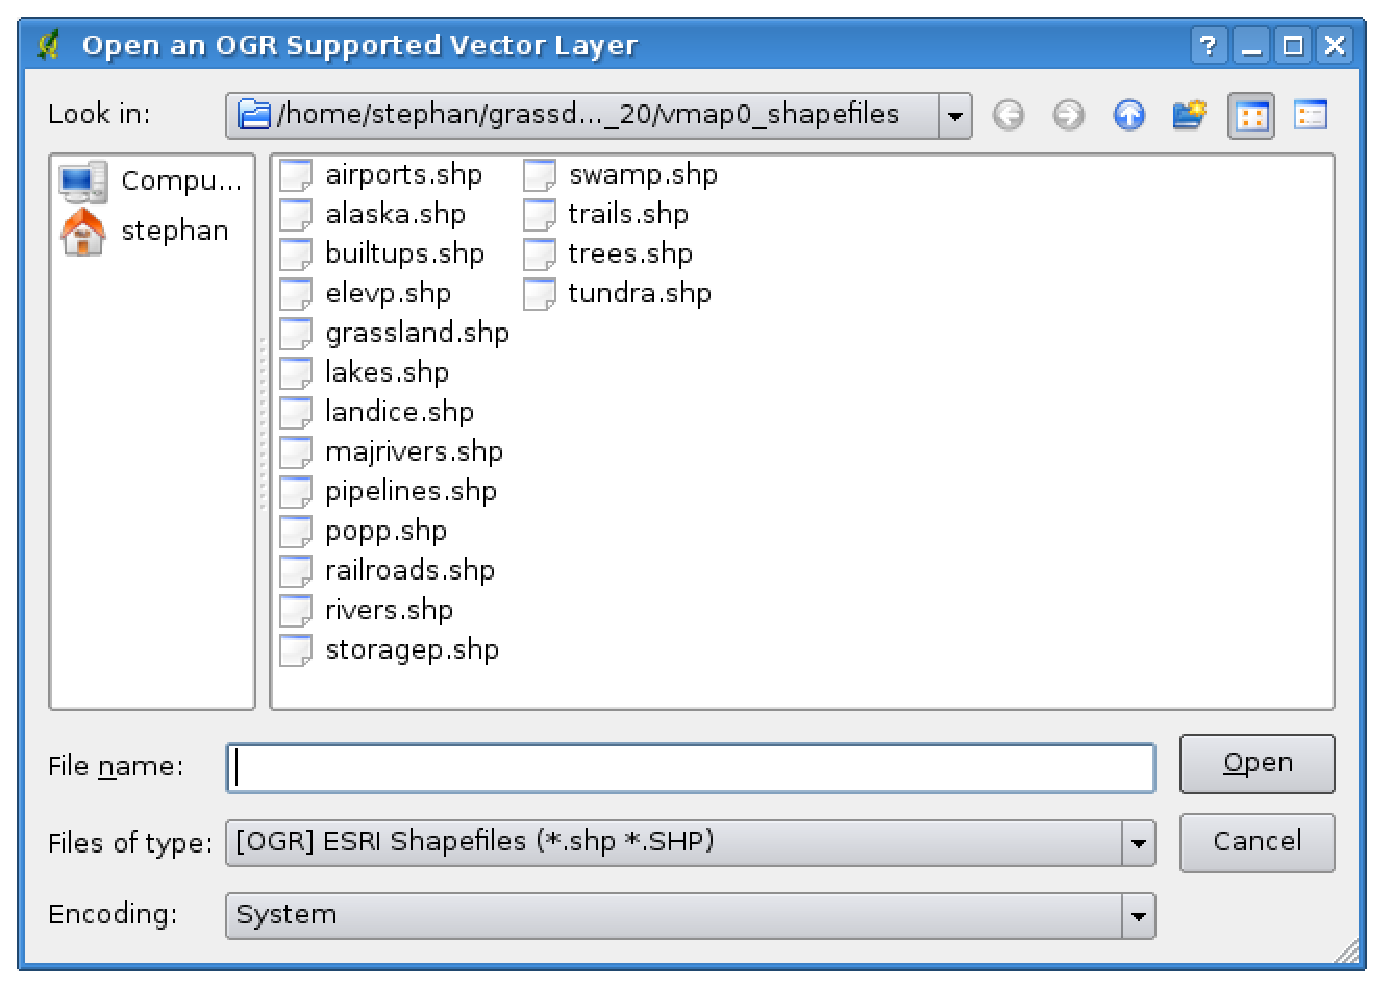
\includegraphics[clip=true, width=14cm]{shapefileopendialog}
\end{center} 
\end{figure}

\begin{figure}[ht]
   \begin{center}
   \caption{QGIS con un shapefile de Alaska cargado \nixcaption}\label{fig:loadedshapefile}\smallskip
   \includegraphics[clip=true, width=16cm]{shapefileloaded}
\end{center} 
\end{figure}

\includegraphics[width=0.7cm]{mActionAddNonDbLayer} Para cargar un shapefile, inicie
QGIS y haga clic en el bot\'on \toolbtntwo{mActionAddNonDbLayer} de la barra de herramientas{A\~nadir una capa vectorial}
\index{shapefile!loading} o simplemente presione la tecla \keystroke{V}. Esto abrir\'a una nueva ventana (vea la Figura \ref{fig:addvectorlayer}).  

De los botones de selecci\'on disponibles verifique \radiobuttonon{Archivo}. Clic en \button{Explorar}. Eso traer\'a un di\'alogo de abrir archivo estandar (vea la Figura \ref{fig:openshapefile}) que permite navegar el sistema de archivos y cargar un  shapefile o cualquier otra fuente de datos soportada. 
La caja de selecci\'on \selectstring{Ficheros de tipo}{\ldots} permite preseleccionar algunos formatos de archivos OGR soportados.

Puede seleccionar tambien el tipo de codificaci\'on deseado para el shapefile.

Seleccionando un shapefile de la lista y haciendo clic en \button{Abrir} lo carga dentro de QGIS. La Figura
\ref{fig:loadedshapefile} muestra QGIS despues de cargar el archivo \filename{alaska.shp}.


\begin{Tip}\caption{\textsc{Colores de la capa}}
\qgistip{Cuando agrega una capa al mapa, se le asigna un color de manera aleatoria. Cuando se
agrega mas de una capa al mismo tiempo, se le asigna diferentes colores a cada capa. }
\end{Tip}

Una vez cargado, puede hacer acercamientos o alejamientos al shapefile usando las herramientas de navegaci\'on del mapa.
Para cambiar la simbolog\'ia de la capa, abra el di\'alogo \dialog{Propiedades de la capa} haciendo doble clic en el nombre de la capa o haciendo clic derecho en el nombre de la capa en la leyenda y eligiendo \dropmenuopt{Propiedades} del men\'u emergente. Vea la  Secci\'on \ref{sec:symbology} para mas informaci\'on sobre como configurar la simbolog\'{\i}a para capas vectoriales.
  
\subsubsection{Mejorando el rendimiento}

Para mejorar el rendimiento del dibujado de un shapefile, puede crear un \'{\i}ndice espacial. Un \'{\i}ndice espacial \index{spatial index!shapefiles} mejorar\'a la velocidad en las operaciones de acercar, alejar y desplazar. Los \'{\i}ndices espaciales usados por QGIS tienen una extensi\'on \filename{.qix}.

Use estos pasos para crear el \'{\i}ndice:

\begin{itemize}
\item Cargue un shapefile.
\item Abra el di\'alogo \dialog{Propiedades de la capa} haciendo doble clic en el nombre del shapefile en la leyenda o haciendo clic derecho en el nombre de la capa en la leyenda y eligiendo \dropmenuopt{Propiedades} del men\'u emergente.
\item En la pesta\~na general \tab{General} haga clic en el bot\'on \button{Crear \'Indice Espacial}.
\end{itemize}

\subsubsection{Cargando una capa de MapInfo}
\index{vector layers!MapInfo}

Para cargar una capa de MapInfo, haga clic en el bot\'on  \toolbtntwo{mActionAddNonDbLayer}{A\~nadir capa vectorial}
de la barra de herramientas o presione la tecla \keystroke{V}, cambie el filtro de tipo de archivo a
\selectstring{Ficheros de tipo}{[OGR] MapInfo (*.mif
*.tab *.MIF *.TAB)} y seleccione la capa que desea cargar.

\subsubsection{Cargando un ArcInfo Binary Coverage}
\index{vector layers!ArcInfo Binary Coverage}

Para cargar un ArcInfo binary coverage haga clic en el bot\'on  
\toolbtntwo{mActionAddNonDbLayer}{A\~nadir capa vectorial} de la barra de herramientas
o presione la tecla \keystroke{V} para abrir el di\'alogo 
\dialog{A\~nadir capa vectorial}.  Seleccione \radiobuttonon{Directorio}. Cambie a \selectstring {Tipo}{Arc/Ingo Binary Coverage}. 
Navegue al directorio que contiene los archivos de coberturas y selecci\'onelo.

Similarmente, puede cargar vectores basados en directorio como el formato UK National Transfer as\'{\i} como el 
formato raw TIGER del US Census Bureau.

\subsection{Capas PostGIS}
\index{vector layers!PostGIS|see{PostGIS}}
\index{PostGIS!layers}
\label{label_postgis} 

Las capas de PostGIS son almacenadas en una base de datos PostgreSQL. Las ventajas de PostGIS
son indexamiento espacial, filtrado y las capacidades de consulta que provee. Usando POstgis, funciones
vectoriales tales como seleccionar e identificar funcionan mucho mas eficazmente que con
capas OGR en QGIS.

Para usar capas de PostGIS debe de:\index{PostgreSQL!loading layers}
\begin{itemize}
\item Crear una conexi\'on almacenada en QGIS a la base de datos PostgreSQL (si no ha sido
previamente definida).\index{PostgreSQL!connection}
\item Conectarse a la base de datos.
\item Seleccionar la capa a agregar al mapa.
\item Opcionalmente proveer una clausula SQL \usertext{where}
para definir que caracter\'{\i}sticas cargar desde la capa.
\item Cargar la capa.
\end{itemize}

\subsubsection{Creando una conexi\'on almacenada}\index{PostgreSQL!connection}\label{sec:postgis_stored}


\includegraphics[width=0.7cm]{mActionAddLayer} La primera vez que utilize un conjunto de datos PostGIS, debe crear una conexi\'on a la base de datos PostgreSQL que contiene los datos. Comienze haciendo clic en el bot\'on \toolbtntwo{mActionAddLayer}{A\~nadir capa de PostGIS} de la barra de herramientas, seleccionando la opci\'on 
\dropmenuopttwo{mActionAddLayer}{A\~nadir capa de PostGIS...} del men\'u \mainmenuopt{Capa} o presionando la tecla \keystroke{D}. Tambien puede abrir el di\'alogo \dialog{A\~nadir capa vectorial} y seleccionar \radiobuttonon{Base de datos}.
Se abrir\'a el di\'alogo \dialog{A\~nadir tabla(s) PostGIS}. Para accesar al manejador de conexiones \index{PostgreSQL!connectionmanager}, haga clic en el bot\'on \button{Nueva} para mostrar el di\'alogo  \dialog{Crear una nueva conexi\'on a PostGIS}. Los par\'ametros requeridos para una conexi\'on se muestran en la tabla \ref{tab:postgis_connection_parms}.

\begin{table}[ht]\index{PostgreSQL!connection parameters}
\centering
\caption{Par\'ametros de conexi\'on a PostGIS}\label{tab:postgis_connection_parms}\medskip
 \begin{tabular}{|l|p{5in}|}
\hline Nombre & Un nombre para esta conexi\'on. Puede ser la misma que \textsl{Base de datos}.
\\
\hline Servidor \index{PostgreSQL!host}
& Nombre del servidor de bases de datos. Este debe ser un nombre de servidor que pueda ser resuelto como puediera
ser usado para abrir una conexi\'on telnet o hacer un ping al servidor. Si la base de datos est\'a 
en la misma computadora que QGIS, simplemente introdusca 'localhost' aqu\'{\i}. \\
\hline Base de datos \index{PostgreSQL!database} & Nombre de la base de datos.  \\
\hline Puerto \index{PostgreSQL!port}& N\'umero del puerto en el que el servidor 
de base de datos PostgreSQL escucha. El puerto por defecto es el 5432.\\
\hline Nombre de Usuario \index{PostgreSQL!username}& El nombre de usuario es usado para iniciar sesi\'on
a la base de datos. \\
\hline Contrase\~na \index{PostgreSQL!password}& Contrase\~na usada para
\textsl{Nombre de usuario} conectarse a la base de datos.\\
\hline Modo SSL \index{PostgreSQL!sslmode}& Como ser\'a negociada la conexi\'on SSL con el servidor. Estas son las opciones: 
\begin {itemize}
\item desactivar: solo tratar una conexi\'on SSL no encriptada;
\item permitir: tratar una conexi\'on sin SSL, si falla, intentar una conexi\'on SSL;
\item preferir (predeterminada): intentar una conexi\'on SSL, si falla, intentar una conexi\'on no-SSL;
\item requerir: solo intentar una conexi\'on SSL.
\end {itemize}
Note se puede alcanzar aumentos masivos en la velocidad de presentado de capas PostGIS desactivando SSL en el editor de conexiones. \\
\hline
\end{tabular}
\end{table}

Opcionalmente puede activar las siguientes casillas:

\begin{itemize}
\item \checkbox{Guardar contrase\~na}
\item \checkbox{Solo buscar en la tabla geometry\_columns}
\item \checkbox{Solo buscar en el esquema 'public'}
\end{itemize}

Una vez que todos los par\'ametros y opciones son establecidos, puede probar la conexi\'on haciendo clic 
en el bot\'on \button{Probar Conexi\'on} \index{PostgreSQL!connection!testing}.

\begin{Tip}\caption{\textsc{Configuraciones de Usuario y Seguridad de QGIS}}\index{settings}\index{security}
\qgistip{Sus configuraciones personalizadas para QGIS son almacenadas en el sistema
operativo. En \nix, las configuraciones son almacenadas en su directorio home en
\filename{.qt/qgisrc}. En \win, las configuraciones son almacenadas en el registro. Dependiendo de su
ambiente de computo, almacenar contrase\~nas en sus configuraciones de QGIS puede ser
un riesgo de seguridad.
}
\end{Tip}

\subsubsection{Cargando una capa PostGIS}\index{PostgreSQL!loading layers}


\includegraphics[width=0.7cm]{mActionAddLayer} Una vez que tiene una o mas
conexiones definidas, puede cargar capas desde la base de datos PostgreSQL. Claro
que esto requiere tener datos en PostgreSQL. Vea la secci\'on
\ref{sec:loading_postgis_data} para una discusi\'on sobre importar datos dentro de la
base de datos. 

Para cargar una capa de PostGIS, realize los siguientes pasos:

\begin{itemize}
\item Si el di\'alogo \dialog{A\~nadir tabla(s) PostGIS} no esta abierto aun, haga clic en el bot\'on
\toolbtntwo{mActionAddLayer}{A\~nadir Capa PostGIS}de la barra de herramientas.
\item Elija la conexi\'on de la lista desplegable y haga clic en \button{Connectar}.
\item Encuentre la capa que desea agregar en la lista de capas disponibles.
\item Seleccionela haciendo clic en ella. Puede seleccionar m\'ultiples capas presionando
la tecla \keystroke{shift} mientras hace clic. Vea la secci\'on \ref{sec:query_builder} para
informaci\'on sobre usar el Constructor de Consultas de PostgreSQL para definir con mas precisi\'on la capa.
\item Clic en el bot\'on \button{A\~nadir} para agregar una capa al mapa.
\end{itemize}

\begin{Tip}\caption{\textsc{Capas PostGIS}}
\qgistip{Normalmente una capa PostGIS es definida por una entrada en la tabla
geometry\_columns. Desde la versi\'on \OLD % should be 0.9.0 
hacia arriba, QGIS puede cargar capas que no tienen una entrada
en la tabla geometry\_columns. Esto incluye tablas y vistas.
La definici\'on de una vista espacial provee poderosos medios para visualizar sus datos. Rem\'{\i}tase
a su manual de PostgreSQL para informaci\'on sobre creaci\'on de vistas.}
\end{Tip}

\subsubsection{Algunos detalles acerca de capas PostgreSQL}\label{sec:postgis_details}
\index{PostgreSQL!layer details}

Esta secci\'on contiene algunos detalles de como QGIS accesa capas PostgreSQL. La mayor\'{\i}a de las veces QGIS deber\'{\i}a simplemente proveerle una lista de tablas de la base de datos que puede ser cargadas, y cargarlas cuando sea necesario. Sin embargo, si tiene problemas cargando una tabla PostgreSQL en QGIS, la siguiente informaci\'on puede ayudarle a entender cualquier mensaje de QGIS y guiarlo para cambiar la definici\'on de tabla o vista de PostgreSQL para que QGIS pueda cargarla.

QGIS requiere que las copas de PostgreSQL contengan una columna que pueda ser usada como llave \'unica para la capa. Para tablas esto usualmente significa que la tabla necesita una llave primaria, o una columna con una restricci\'on de \'unica en ella. En QGIS, esta columna necesita ser del tipo int4 (un entero de tama\~no de 4 bytes). Alternativamente una columna ctid puede ser usada como llave primaria. Si la tabla carece de estos elementos, la columna oid ser\'a usada. El rendimiento se mejorar\'a si la columna es indexada (note que las llaves primarias son indexadas autom\'aticamente en PostgreSQL). 

Si la capa PostgreSQL es una vista, existe el mismo requerimiento, pero las vistas no tienen llave primaria o columnas restricciones de valores \'unicos. En este caso QGIS tratar\'a de encontrar una columna en la vista que sea derivada de una columna adecuada. La determinaci\'on de la columna se hace analizando la definici\'on SQL de la vista. Sin embargo hay varios aspectos de SQL que QGIS ignora - estos incluyen el uso de alias en tablas y columnas que son generados por funciones SQL.

Si no es posible encontrar una columna adecuada, QGIS no cargar\'a la capa. Si esto ocurre, la soluci\'on es alterar la vista de manera que incluya una columna adecuada (de un tipo int4 y que bien sea una llave primaria o que tenga una restricci\'on de valores \'unicos en la columna, preferentement indexada). 

Cuando QGIS trabaja con vistas, analiza la definici\'on de la vista y 

\subsubsection{Importando datos a PostgreSQL}\label{sec:loading_postgis_data} \index{PostGIS!SPIT!importing data} \minisec{shp2pgsql}
Los datos pueden ser importados a PostgreSQL usando un n\'umero de m\'etodos. PostGIS
incluye una utiler\'{\i} llamada \filename{shp2pgsql} que puede ser usada para importar shapefiles a una base de datos PostgreSQL con PostGIS activado. Por ejemplo para importar un shapefile llamado \filename{lakes.shp} a una base de datos PostgreSQL llamada \usertext{gis\_data}, use el siguiente comando:

\begin{verbatim} 
  shp2pgsql -s 2964 lakes.shp lakes_new | psql gis_data
\end{verbatim}

Esto crea una capa llamada \usertext{lakes\_new} en la base de datos \usertext{gis\_data}. La nueva capa tendr\'a un identificador del sitema espacial de referencia (SRID) de 2964. Vea la secci\'on \ref{label_projections} para mas informaci\'on de sistemas de referencia espaciales y proyecciones.

\begin{Tip}
\caption{\textsc{Exporting datasets from PostGIS}\index{PostGIS!Exporting}}
\qgistip{Al igual que la herramienta de importaci\'on \filename{shp2pgsql} hay tambien una herramienta para exportar
conjuntos de datos PostGIS a shapefiles: \filename{pgsql2shp}. Esta se encuentra en 
su distribuci\'on PostGIS.} 
\end{Tip}

\minisec{SPIT Plugin}

\includegraphics[width=0.7cm]{spiticon} QGIS viene con un complemento llamado 
SPIT (Shapefile to PostGIS Import Tool)\index{PostGIS!SPIT}.
SPIT puede ser usado para cargar m\'ultiples shapefiles al mismo tiempo e inluye soporte para esquemas. Para usar SPIT, habra el Manejador de Complementos del men\'u \mainmenuopt{Plugins}, verifique la caja siguiente al \checkbox{SPIT plugin} y haga clic en el bot\'on \button{OK}. El \'{\i}cono de SPIT ser\'a agregado a la barra de herramientas de complementos \index{PostGIS!SPIT!loading}. 

Para importar un shapefile, haga clic en \'{\i}cono de la barra de herramientas \toolbtntwo{spiticon}{SPIT} para abrir el di\'alogo \dialog{SPIT - Shapefile to PostGIS Import Tool}. Seleccione la base de datos PostGIS a la que desea conectarse y haga clic en el bot\'on \button{Connect}. Ahora puede agregar uno o mas archivos a la cola haciendo clic en el bot\'on   \button{Add}. Para procesar los archivos, haga clic en el bot\'on  
\button{OK}. El progreso de la importaci\'on as\'{i} como cualquier error\\advertencia ser\'a mostrado conforme cada shapefile sea procesado.

\begin{Tip}\caption{\textsc{Importing Shapefiles Containing
PostgreSQL Reserved Words}}\index{PostGIS!SPIT!reserved words}
\qgistip{ Si es agregado un shapefile que contenga campos que sean palabras reservadas en el PostgreSQL se abrir\'a un di\'alogo mostrando el estado de cada campo. Los nombres de los campos pueden ser editados\index{PostGIS!SPIT!editing field names} antes de importarr y cambiar cualquier palabra reservada ( o cualquier otro nombre de campos que se desee). Intentar importar un shapefile con palabras reservadas como nombres de campos fallar\'a.}
\end{Tip} 

\minisec{ogr2ogr}
Ademas de \filename{shp2pgsql} y \filename{SPIT} hay otra herramienta para alimentar datos espaciales al PostGIS: \filename{ogr2ogr}. Esta herramienta es parte de la instalaci\'on de GDAL.
Para importar un shapefile a PostGIS, haga lo siguiente:
\begin{verbatim}
  ogr2ogr -f "PostgreSQL" PG:"dbname=postgis host=myhost.de user=postgres \
  password=topsecret" alaska.shp
\end{verbatim}

Esto importar\'a un shapefile  llamado \filename{alaska.shp} dentro de la base de datos PostGIS
\usertext{postgis}
usando el usuario \usertext{postgres} con ls contrase\~na \usertext{topsecret} en el servidor
\server{myhost.de}.

Note que OGR debe ser compilado con PostgreSQL para soportar PostGIS.
Esto se puede ver escribiendo
\begin{verbatim}
ogrinfo --formats | grep -i post
\end{verbatim}

Si desea utilizar comandos de PostgreSQL \filename{COPY}- en lugar del default
\filename{INSERT INTO} puede exportar la siguiente variable de ambiente( al menos disponible en \nix y \osx):
\begin{verbatim}
  export PG_USE_COPY=YES
\end{verbatim}

\filename{ogr2ogr} no crea \'{\i}ndices espaciales por defecto como lo hace \filename{shp2pgsl}. Necesita crearlos manualmente usando el comando SQL \filename{CREATE INDEX} despues como una paso extra (como se describe en la siguiente secci\'on \ref{label_improve}).

\subsubsection{Mejorando el rendimiento} \label{label_improve}

Recuperar caracter\'{\i}sticas de una base de datos PostgreSQL puede ser tardado, especialmente si se trabaja en red. Se puede mejorar el rendimiento del dibujado de capas PostgreSQL asegurando que exista un \'{\i}ndice espacial \index{PostGIS!spatial index} en cada capa de la base de datos. PostGIS suporta la creaci\'on de \'{\i}ndices GiST (Generalized Search Tree) \index{PostGIS!spatial index!GiST} para agilizar consultas espaciales de los datos.

La sintaxis para crear un \'{\i}ndice GiST\footnote{La informaci\'on de \'{\i}ndices GiST es tomada de la documentaci\'on de PostGIS
disponible en \url{http://postgis.refractions.net}}
es:

\begin{verbatim}
    CREATE INDEX [indexname] ON [tablename] 
      USING GIST ( [geometryfield] GIST_GEOMETRY_OPS );
\end{verbatim}

Note que para tablas grandes, la creaci\'on de un \'{\i}ndice puede tomar mucho tiempo. Una vez
el \'{\i}ndice es creado, debe realizarse un \usertext{VACUUM ANALYZE}. Vea la documentaci\'on de
PostGIS \cite{PostGISweb} para mas informaci\'on.

El siguiente es un ejemplo de la creaci\'on de un \'{\i}ndice GiST:
\begin{verbatim}
gsherman@madison:~/current$ psql gis_data
Welcome to psql 8.3.0, the PostgreSQL interactive terminal.

Type:  \copyright for distribution terms
        \h for help with SQL commands
        \? for help with psql commands
        \g or terminate with semicolon to execute query
        \q to quit

gis_data=# CREATE INDEX sidx_alaska_lakes ON alaska_lakes
gis_data-# USING GIST (the_geom GIST_GEOMETRY_OPS);
CREATE INDEX
gis_data=# VACUUM ANALYZE alaska_lakes;
VACUUM
gis_data=# \q
gsherman@madison:~/current$
\end{verbatim}

\subsection{Capas SpatiaLite} 
\index{SpatiaLite layers!properties dialog}
\index{vector layers!SpatlaLIte|see{SpatiaLite}}
\index{SpatiaLite!layers}
\label{label_spatialite} 

\includegraphics[width=0.7cm]{mActionAddSpatiaLiteLayer}
Para cargar datos desde una base de datos Spatialite, comienze haciendo clic en el bot\'on de la barra 
de herramientas \toolbtntwo{mActionAddSpatiaLiteLayer}{Add SpatiaLite Layer} o seleccionando la opci\'on  
\dropmenuopttwo{mActionAddSpatiaLiteLayer}{Add SpatiaLite Layer...} 
\mainmenuopt{Layer} del men\'u o tecleando \keystroke{L}. 
Esto mostrar\'a una ventana, la cual permitir\'a que se conecte a una base de datos Spatialite conocida por QGIS, la cual 
puede ser seleccionada del men\'u desplegable o definir una nueva conecci\'on a una base de datos. Para definir una nueva conecci\'on, haga clic en \button{New} y use el bavegador de archivos para apuntar hacia su base de datos SpatiaLite, 
el cual es un archivo con una extensi\'on \filename{.sqlite }.

\subsection{El di\'alogo de propiedades de vectores}\label{sec:vectorprops}
\index{vector layers!properties dialog}

El di\'alogo \dialog{Layer Properties} para una capa vectorial 
provee informaci\'on acerca de la capa, configuraciones
de simbolog\'{\i} y opciones de etiquetado. Si la capa vectorial ha sido cargada desde
un almacen de datos PostgreSQL / PostGIS, tambien puede alterar el SQL subyacente para la
capa - bien manualmente editando el SQL en la pesta\~na \tab{General} o invocando
el di\'alogo \dialog{Query Builder} en la pesta\~na \tab{General}. 
Para accesar al di\'alogo
\dialog{Layer Properties}, haga doble clic en un capa en la leyenda o clic derecho sobre
la capa y seleccionela del men\'u emergente \dropmenuopt{Properties}.

\begin{figure}[H]
   \begin{center}
   \caption{Di\'alogo de Propiedades de Capas Vectoriales \nixcaption}\label{fig:vector_symbology}\smallskip
   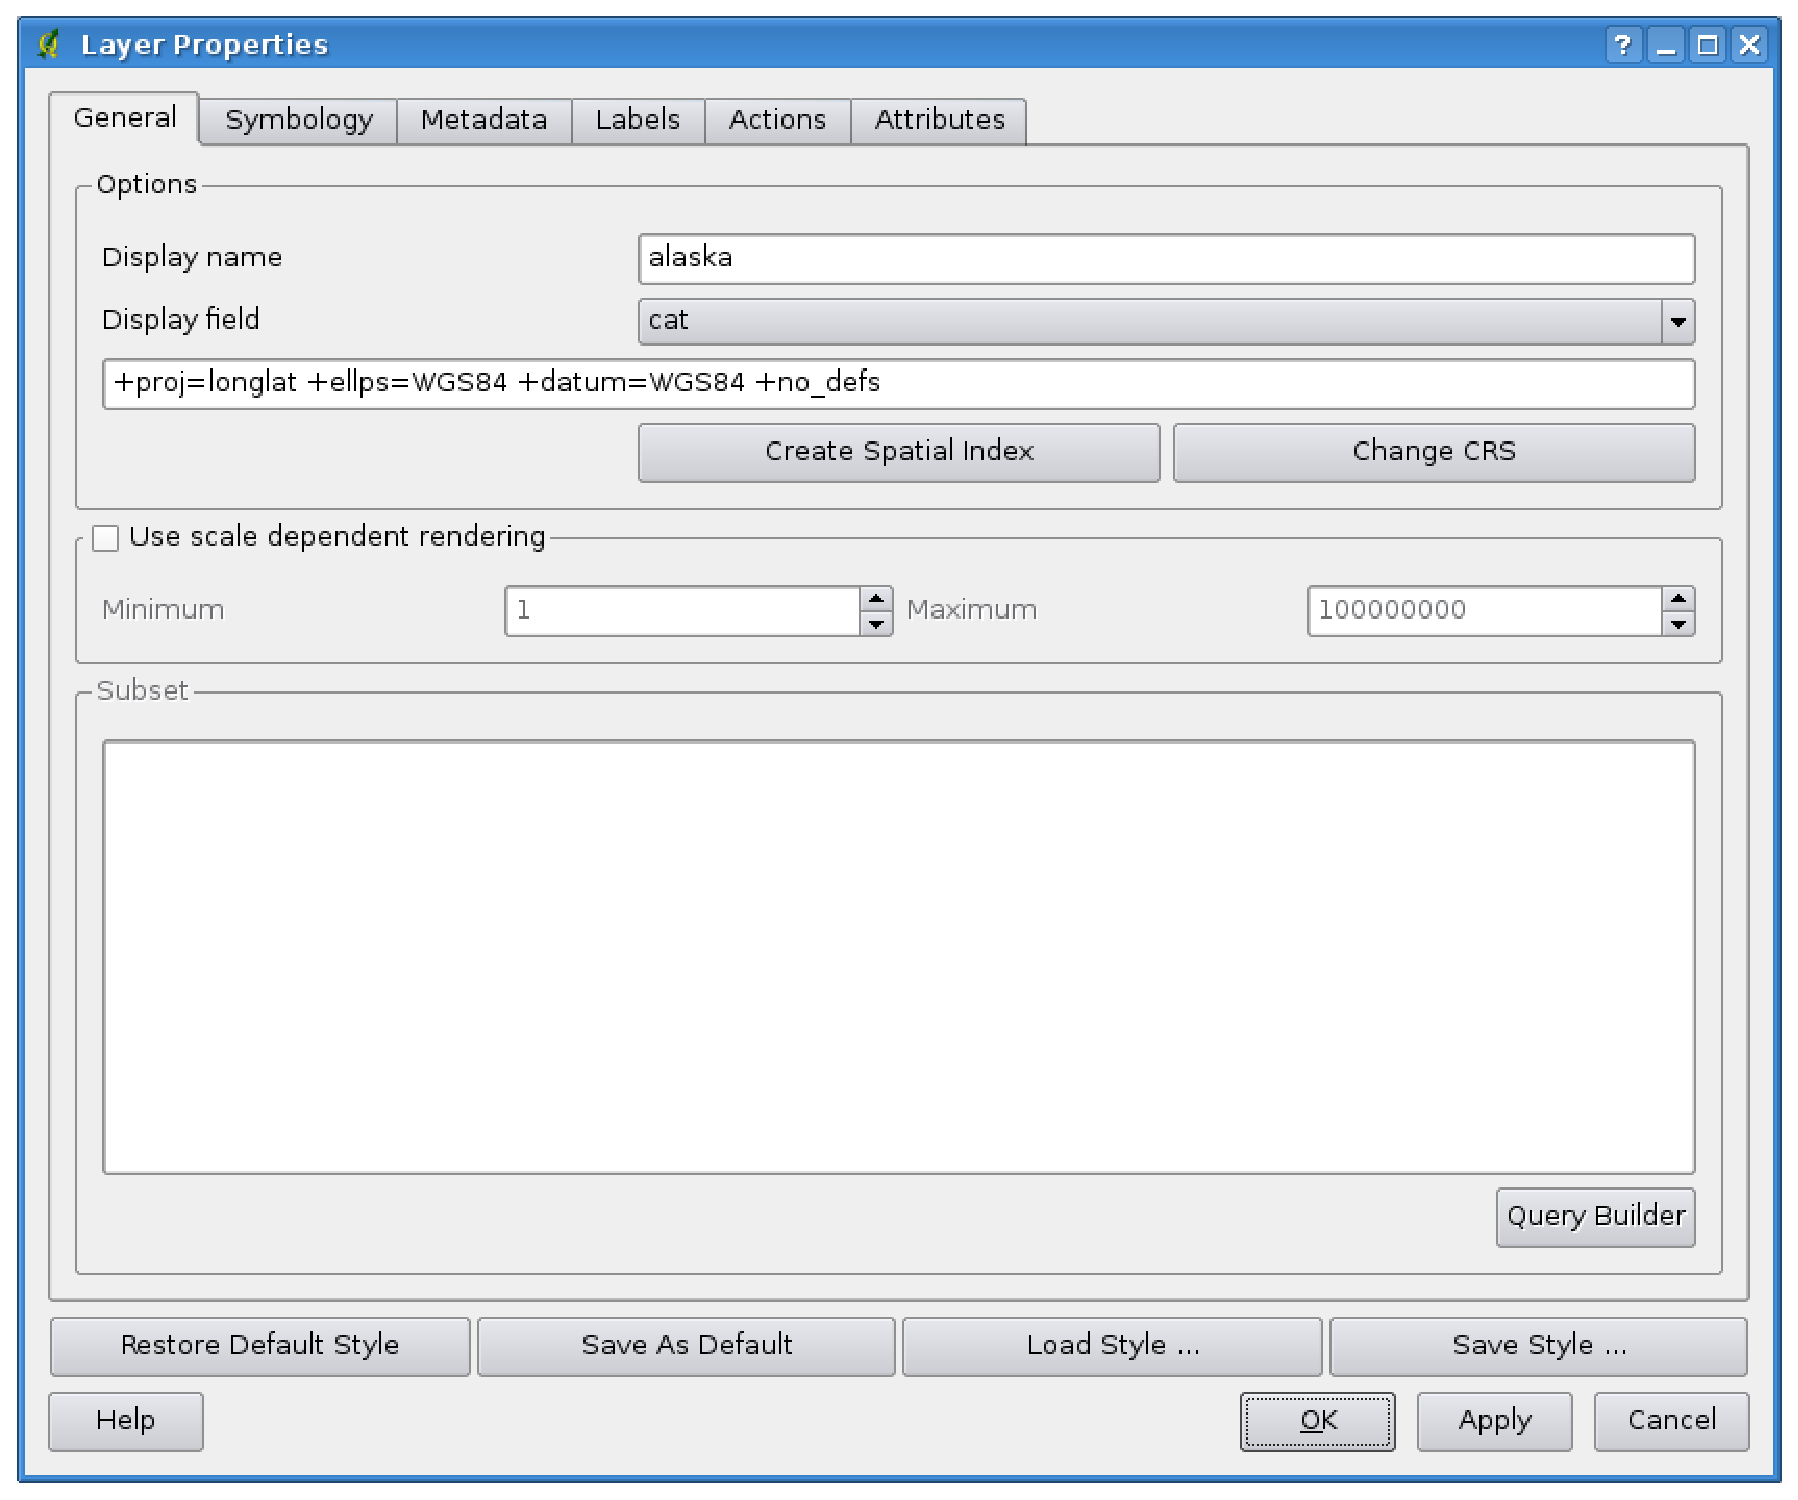
\includegraphics[clip=true, width=12cm]{vectorLayerSymbology} 
\end{center}  
\end{figure}

\subsubsection{Pesta\~na general}\label{vectorgeneraltab}
La pesta\~na \tab{General} es esencialmente muy parecida a la del di\'alogo raster. Permite
cambiar el nombre a mostrar, establecer las opciones de dibujado dependientes de la escala, crear un \'{\i}ndice espacial 
de el archivo vectorial (solo para formatos OGR y PostGIS) y ver o cambiar
la proyecci\'on espec\'{\i}fica para la capa vectorial.

El bot\'on \button{Query Builder} permite crear un subconjunto de caracter\'{\i}sticas 
en la capa - pero este bot\'on actualmente solo est\'a disponible cuando se abre la tabla  
de atributos y se selecciona el bot\'on \button{...} siguiente a b\'usqueda avanzada.

\subsubsection{Pesta\~na simbolog\'{\i} Tab}\label{sec:symbology}
\index{vector layers!symbology}

QGIS soporta un n\'umero de renderers simbolog\'{\i}as para controlar como
los caracter\'{\i}sticas vectoriales son mostradas. Actualmente los siguientes renderers
est\'an disponibles:

\begin{description} 
    \item[S\'{\i}mbolo simple] - un solo estilo es aplicado a
    cada objeto en la capa.\index{vector layers!renderers!single symbol}
    \item[S\'{\i}mbolo graduado] - los objetos dentro de la capa son
    mostrados con diferentes s\'{\i}mbolos clasificados por los valores de un
    campo particular. \index{vector layers!renderers!graduated symbol}
    \item[Color cont\'{\i}nuo] - los objetos dentro de la capa son
    mostrados con una propagaci\'on de colores clasificado por los valores
    n\'umericos de un campo espec\'{\i}fico.\index{vector layers!renderers!continuous
color}
    \item[Valor \'unico] - los objetos son clasificados por los valores \'unicos
    dentro de un campo especificado teniendo cada valor un diferente s\'{\i}mbolo.
    \index{vector layers!renderers!unique value}
\end{description}

Para cambiar la simbolog\'{\i}a de una capa, simplemente has doble clic en su entrada
en la leyenda y el di\'alogo de propiedades del vector \dialog{Layer Properties} se mostrar\'a.\index{symbology!changing}

\begin{figure}[h]
\centering
\caption{Symbolizing-options \nixcaption}
   \subfigure[S\'{\i}mbolo simple] {\label{subfig:single_symbol}\includegraphics[clip=true, width=0.4\textwidth]{vectorClassifySingle}}\goodgap
   \subfigure[S\'{\i}mbolo graduado] {\label{subfig:graduated_symbol}\includegraphics[clip=true, width=0.4\textwidth]{vectorClassifyGraduated}}\\
   \subfigure[Color cont\'{\i}nuo] {\label{subfig:cont_color}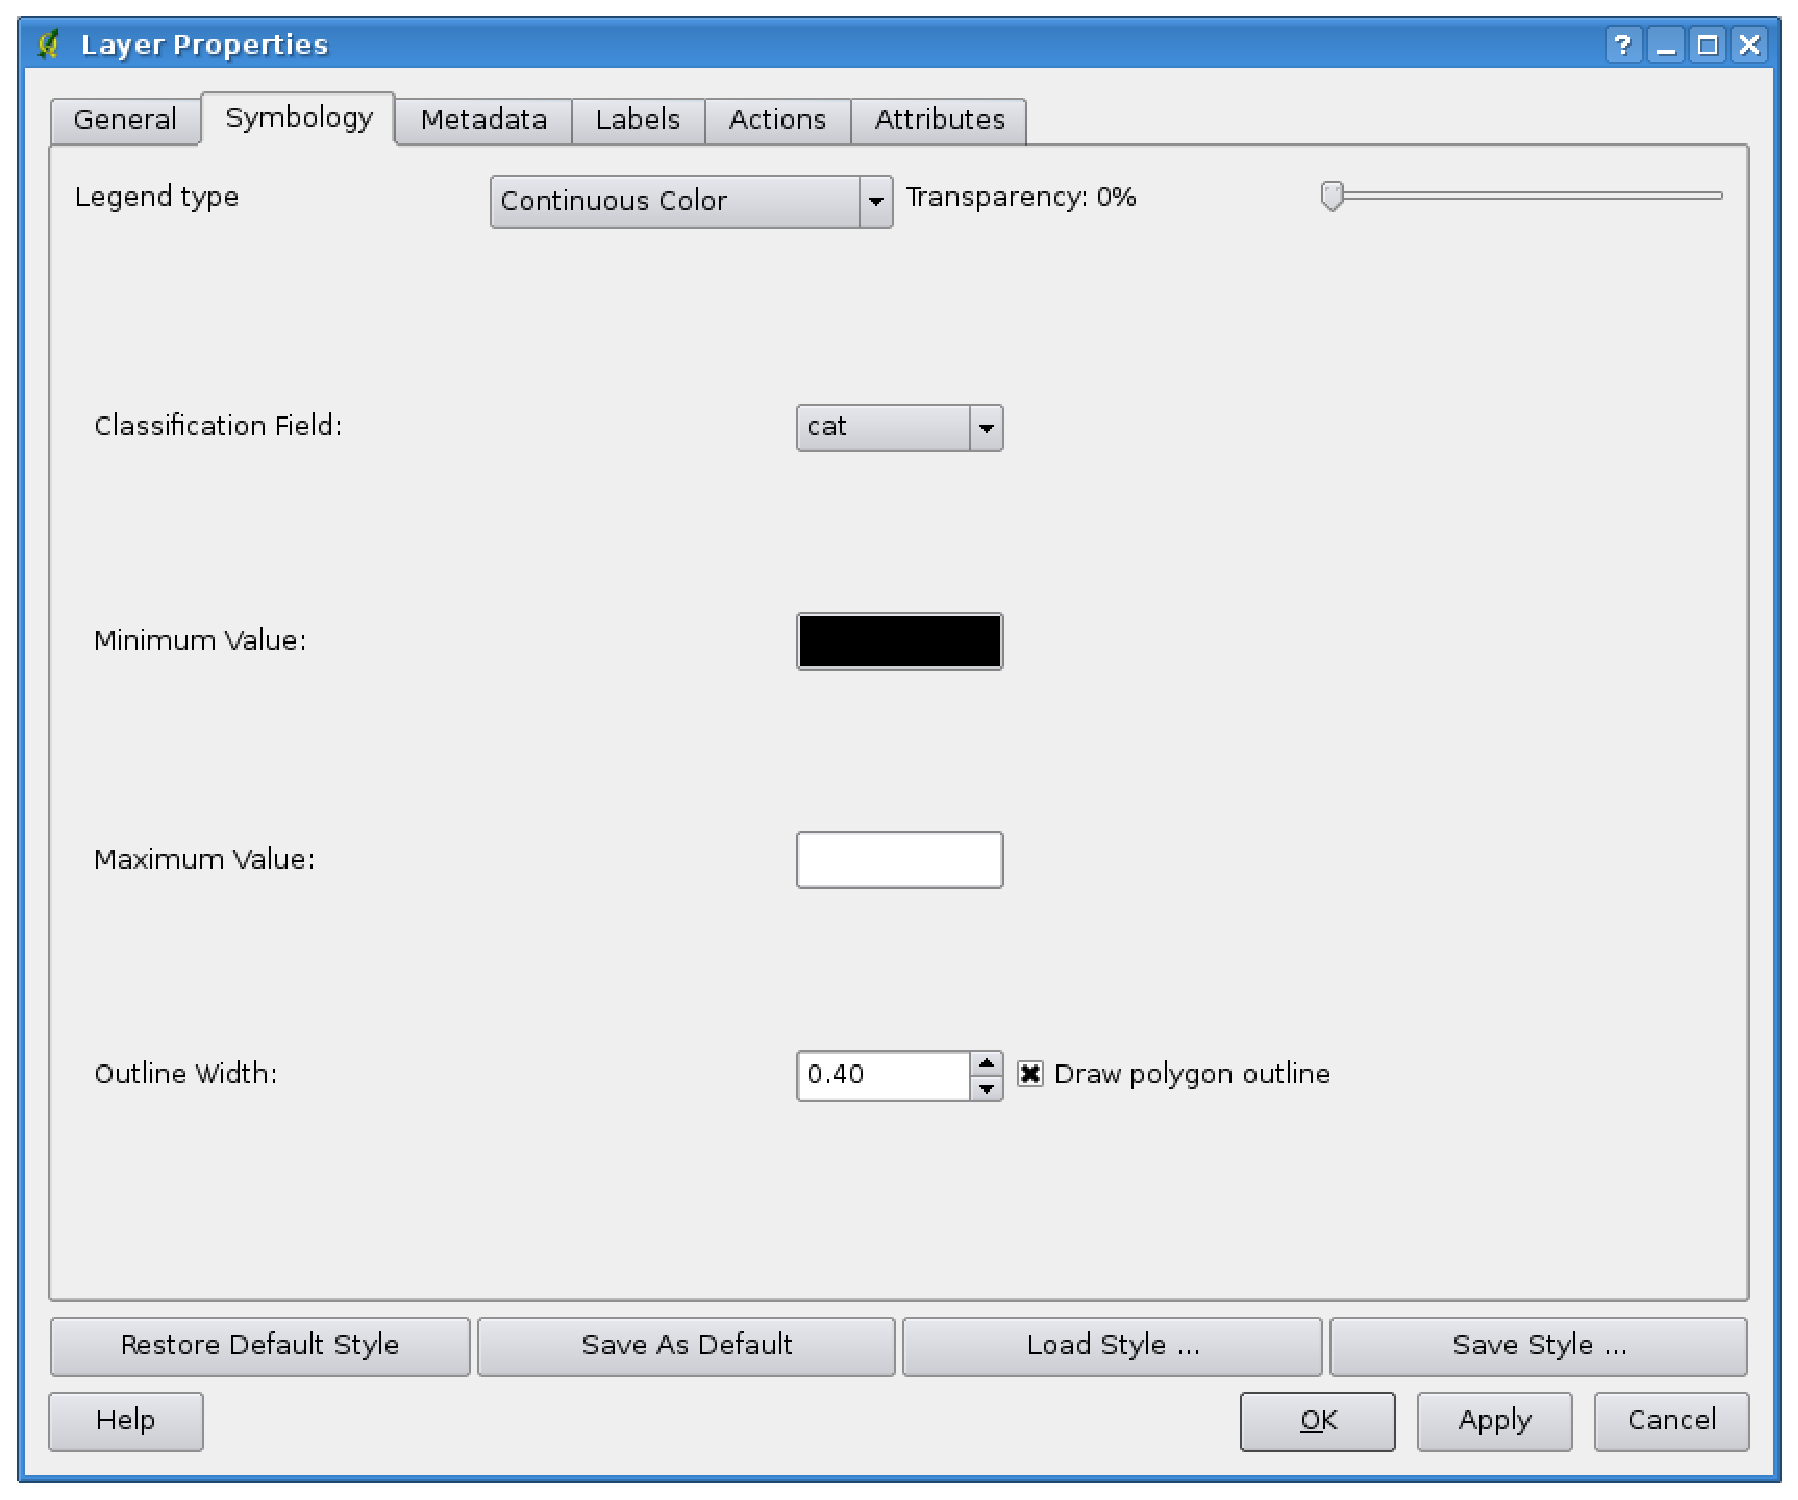
\includegraphics[clip=true, width=0.4\textwidth]{vectorClassifyContinous}}\goodgap
   \subfigure[Valor \'unico] {\label{subfig:unique_val}\includegraphics[clip=true, width=0.4\textwidth]{vectorClassifyUnique}}
\end{figure}

% FIXME: outdated
% Since \usertext{version v0.9} there is a function to use image files stored on 
% your computer as fill pattern for vector layers.

\minisec{Style Options} \label{sec:style_options} \index{vector layers!styles}
Dentro de este di\'alogo se puede definir el estilo de la capa vectorial. Dependiendo de la opci\'on
seleccionada de dibujado tambien es posible clasificar caracter\'{\i}sticas del mapa.

Al menos las siguientes opciones de estilo pueden aplicarse para casi todos los renderers:
\begin{description}
 \item[Estilo de borde] - estilo de lapiz para el borde de las caracter\'{\i}sticas. Tambien puede ser
 establecido a 'sin lapiz'.
 \item[Color de borde] - color del borde de las caracter\'{\i}sticas.
 \item[Ancho de borde] - ancho del borde de las caracter\'{\i}sticas.
 \item[Color de relleno] - color de relleno de las caracter\'{\i}sticas.
 \item[Estilo de relleno] - estilo para el relleno. Aparte de las brochas definidas puede
 seleccionar \selectstring{Fill style}{? texture} y hacer clic en el bot\'on \browsebutton
 para seleccionar su propio estilo de relleno. Actualmente los formatos soportados son
 \filename{*.jpeg, *.xpm, and *.png}.
\end{description}

Una vez que ha estilizado su capa tambien puede almacenar su estilo de capa a
un archivo separado (con extensi\'on \filename{*.qml}).
Para hacer esto, use el bot\'on \button{Save Style \ldots}. No hay necesidad de decir que
\button{Load Style \ldots} carga el archivo de estilo previamente almacenado.

Si se desea siempre usar un estilo particular siempre que la capa es cargada, 
use el bot\'on \button{Save As Default} para hacer su estilo el estilo por defecto. Tambien, 
si hace cambios al estilo y no esta contento con los cambios, use el bot\'on \button{Restore 
Default Styel} para revertir a su estilo por defecto.

\minisec{Transparencia de vectores} \label{sec:vect_transparency} \index{vector layers!transparency}
QGIS \CURRENT soporta el establecer transparencia para cada capa vectorial. Esto puede ser hecho con
la barra de desplazamiento \slider{Transparency}{0}{20mm} dentro de la pesta\~na \tab{symbology} (vea la fig. \ref{fig:vector_symbology}).
Esto es muy \'util para sobreponer varias capas vectoriales.

\subsubsection{Pesta\~na metadatos}

La pesta\~na \tab{Metadata} contiene informaci\'on acerca de la capa, incluyendo peculiaridades
acerca del tipo y localizaci\'on, n\'umero de caracter\'{\i}sticas, tipo de caracter\'{\i}stica, y las capacidades de edici\'on.
La Secci\'on \guiheading{Layer Spatial Reference System}, provee 
informaci\'on de proyecci\'on, y la secci\'on \guiheading{Attribute field info},
lista los campos y sus tipos de datos. Esta es una forma r\'apida de obtener informaci\'on acerca de la capa.

\subsubsection{Pesta\~na etiquetas}

La pesta\~na \tab{Labels} permite activar el etiquetado de caracter\'{\i}sticas y controlar un n\'umero de opciones
relacionadas con las fuentes, colocaci\'on, estilo, alineaci\'on y buffering.

Vamos a ilustrar esto etiquetando el shapefile lakes de el 
\filename{qgis\_example\_dataset}:

\begin{enumerate}
\item Cargar el shapefile \filename{alaska.shp} y el archivo GML \filename{lakes.gml} en QGIS.
\item Acerquese un poco a su area favorita con alg\'un lago.
\item Haga la capa \filename{lakes} la capa activa.
\item Abra el di\'alogo \dialog{Layer Properties}.
\item Clic en la pesta\~na \tab{Labels}.
\item Verifique la caja de selecci\'on \checkbox{Display labels} para activar el etiquetado.
\item Elija el campo a usar en el etiquetado. 
  Usaremos \selectstring{Field containing label}{NAMES}.
\item Escriba un valor por defecto para lagos que no tengan nombre. La etiqueta por defecto ser\'a
  usada cada vez que QGIS encuentre un lago sin valor en el campo \guilabel{NAMES}.
\item Si tiene etiquetas que se extienden sobre varia l\'{\i}neas, verifique \checkbox{Multiline labels?}. 
QGIS verificar\'a una verdadera l\'{\i}nea sea regresada en su campo etiqueta e inserta retornos de l\'{\i}nea como corresponda.
Una verdadera l\'{\i}nea regresada es un caracter \textbf{single} \textbackslash n, 
(no dos caracteres separados, como una diagonal invertida \textbackslash ~seguida del caracter n).
\item clic en el bot\'on \button{Apply}.
\end{enumerate} 

Ahora tenemos etiquetas. Como se ven? Probablemente muy grander y pobremente colocadas en relaci\'on al s\'{\i}mbolo
marcador para los lagos.

Seleccione la entrada \tab{Font} y use los botones  \button{Font} y \button{Color}
para establecer la fuente y el color. Tambien puede cambiar el \'angulo y la posici\'on de la etiqueta de texto.


Para cambiar la posici\'on del texto relativo a la caracter\'{\i}stica:

\begin{enumerate} 
\item Hacen clic en la entrada \tab{Font}.
\item Cambiar el posicionamiento seleccionando uno de los botones de selecci\'on
en el grupo \classname{Placement}. Para fijar las etiquetas, elija el bot\'on de selecci\'on
\radiobuttonon{Right}.
\item el \classname{Font size units} permite seleccionar entre
\radiobuttonon{Points} o \radiobuttonon{Map units}.
\item Haga clic \button{Apply} para ver los cambios sin cerrar el di\'alogo.
\end{enumerate} 

Las cosas se ven mejor, pero las etiquetas est\'an aun muy cerca del marcador. Para
arreglar esto podemos usar las opciones en la entrada \tab{Position}. Aqu\'{\i} podemos agregar 
desplazamientos en las direcciones X y Y. Agregando un desplazamiento de 5 mover\'a las etiquetas
fuera del marcador y las har\'a mas legibles. Claro esto si el s\'{i}mbolo marcador
o la fuente es muy grande, ser\'a necesario un desplazamiento mayor.

El \'ultimo ajuste que haremos es \tab{buffer} las etiqueta. Esto significa
poner un fondo alrededor de ellas para que se vean mejor. Para hacer un buffer a las
etiquetas de lagos:

\begin{enumerate}
\item Clic en la pesta\~na \tab{Buffer}.
\item Clic en la casilla de verificaci\'on  \checkbox{Buffer Labels?} para activar el buffering.
\item Elija el tama\~no del buffer usando el spin box.
\item Elija un color haciendo clic en \button{Color} y eligiendo el color favorito
  con el selector de colores. Puede establecer alguna transparencia para el buffer
  si lo prefiere.
\item Clic \button{Apply} para ver si los cambios le agradan.
\end{enumerate} 

Si no est\'as feliz con los resultados, afine las configuraciones y pruebe nuevamente
haciendo clic en \button{Apply}.

Un buffer de un 1 punto parece dar un buen resultado.
Note que puede tambien especificar un tama\~no de buffer en unidades de mapa si eso trabaja mejor
para usted.

Las entradas restantes en la pestan\~a \tab{Label} permiten controlar la apariencia de las
etiquetas usando atributos almacenados en la capa. Las entradas que comienzan con \tab{Data defined} permiten establecer
todos los par\'ametros para las etiquetas usando campos de la capa.

Note que la pesta\~na \tab{Label} que provee \classname{preview-box} donde 
se muestra la etiqueta seleccionada.

\subsubsection{Pesta\~na acciones}\index{actions}\label{label_actions}

QGIS provee la habilidad de realizar una acci\'on basada en los atributos de una
caracter\'{\i}stica. Puede ser usado para realizar cualquier numero de acciones, por ejemplo,
correr un programa con argumentos creados a partir de los atributos de una caractar\'{\i}stica o
pasando argumentos a una herramienta de reporte web.

Las acciones son muy \'utiles cuando se desea correr una aplicaci\'on externa o ver
una p\'agina web basada en uno o mas valores en su capa vectorial. Un ejemplo
is realizar una b\'usqueda basada en un valor de atributo. Este concepto es usado en la  
siguiente discuci\'on.

\minisec{Defining Actions}\index{actions!defining}

Las acciones de atributos son definidas desde el di\'alogo de vectores \dialog{Layer Properties}. Para definir una
acci\'on, abra el di\'alogo de vectores \dialog{Layer Properties} y haga clic en la
pesta\~na \tab{Actions}. Provea un nombre descriptivo para la acci\'on. La acci\'on por si misma
debe contener el nombre de la aplicaci\'on que ser\'a ejecutada cuando la acci\'on es invocada.
Puede agregar uno o mas valores de atributos como argumentos
a la aplicaci\'on. Cuando la acci\'on es invocada cualquier conjunto de caracteres que empiezan
con un \% seguido del nombre de un campo ser\'an reemplazados por el valor de ese campo.
Los caracteres especiales \%\% \index{\%\%}ser\'an reemplazados por el valor
de el campo que fue seleccionado desde identificar resultados o tabla de atributos (vea
Usando Acciones abajo).  Pueden ser usadas comillas dobles para agrupar texto dentro
de un solo argumento para el programa, script o comando. Las comillas dobles ser\'an ignoradas
si est\'an precedidas por una diagonal invertida.

Si tiene nombres de campos que son subcadenas de otros nombres de campos (e.g., \usertext{col1}
y \usertext{col10}) deber\'{\i}a de indicarlos
, rodeando el nombre de campo (y el \% character) con 
corchetes (ej., \usertext{[\%col10]}). Esto prevendr\'a que el nombre de campo \usertext{\%col10}
sea confundido con el nombre de campo \usertext{\%col1} con un \usertext{0}
al final. Los par\'entesis ser\'an removidos por QGIS cuando substituya el valor en el campo
. Si quiere que el campo substituido sea rodeado de corchetes,
use un segundo conjunto como este: \usertext{[[\%col10]]}.

El di\'alogo \dialog{Identify Results} incluye un {\em (Derived)} elemento que
contiene informaci\'on relevante al tipo de capa. Los valores
en este elemento pueden ser accesados en una forma similar a los otros campos
precediendo el nombre de campo derivado  con \usertext{(Derived).}. Por
ejemplo, una capa de puntos tiene un campo \usertext{X} y \usertext{Y} y el
valor de estos puede ser usado en la acci\'on con \usertext{\%(Derived).X} y
\usertext{\%(Derived).Y}. Los atributos derivados est\'an solo disponibles desde el di\'alogo
\dialog{Identify Results}, no en el di\'alogo \dialog{Attribute Table}.

Dos ejemplos de acciones se muestrab abajo:\index{actions!examples}

\begin{itemize}
  \item \usertext{konqueror http://www.google.com/search?q=\%nam}
  \item \usertext{konqueror http://www.google.com/search?q=\%\%}
\end{itemize}

En el primer ejemplo, el navegador konqueror es invocado y pasado a la URL al 
abrirse. La URL realiza una b\'usqueda en Google con el valor del campo \usertext{nam}
de nuestra capa vectorial. Note que la aplicaci\'on o script llamado por la acci\'on
debe ser definida en la ruta o debe proveer la  ruta completa. Para asegurar, podemos
reescribir el primer ejemplo como: \usertext{/opt/kde3/bin/konqueror
http://www.google.com/search?q=\%nam}. Esto asegurar\'a que la aplicaci\'on konqueror
ser\'a ejecutada cuando la acci\'on es invocada.

El segundo ejemplo usa la notaci\'on \%\% que no recae en un campo en particular
para su valor. Cuando la acci\'on es invocada, el \%\% ser\'a reemplazado por
el valor del campo seleccionado en identificar resultados o tabla de atributos.

\minisec{Usando Acciones}\index{actions!using}\label{label_usingactions}
Las acciones pueden ser invocadas bien desde el di\'alogo \dialog{Identify Results} o el 
 di\'alogo \dialog{Attribute Table}. 
(Recuerde que estos di\'alogos pueden ser abiertos haciendo clic en
\toolbtntwo{mActionOpenTable}{Identify Features}
o
\toolbtntwo{mActionOpenTable}{Open Table}.)
Para invocar una acci\'on, 
haga clic derecho en el registro
y elija la acci\'on desde el men\'u emergente. Las acciones se listan en el men\'u
emergente por el nombre que le asign\'o cuando defin\'{\i}a las acciones. Clic en la acci\'on
que desea invocar.

Si est\'a invocando una acci\'on que usa la notaci\'on \%\%, haga clic derecho en el
valor del campo en el di\'alogo \dialog{Identify Results} o el
\dialog{Attribute Table} di\'alogo que desea pasar a la aplicaci\'on o script.

Aqui est\'a un ejemplo que jala datos de una capa vectorial y los inserta
dentro de un archivo usando bash y el comando \usertext{echo} (de esta manera solo trabajar\'a
\nix o quiza \osx). La capa en cuestion tiene campos para nombres de especies
\usertext{taxon\_name}, latitud \usertext{lat} y longitud
\usertext{long}. Desear\'{\i} poder hacer
una selecci\'on espacial de las localidades y exportar estos valores de campos a
un archivo de texto para el registro seleccionado (se muestra en amarillo en el \'area de mapa de QGIS). Aqu\'{\i} est\'a
una acci\'on para lograr esto:

\begin{verbatim}
  bash -c "echo \"%taxon_name %lat %long\" >> /tmp/species_localities.txt"
\end{verbatim} 

Despues de seleccionar algunas localidades y correr una acci\'on en cada una, al abrir
el archivo de salida mostrar\'a algo como esto:

\begin{verbatim}
  Acacia mearnsii -34.0800000000 150.0800000000
  Acacia mearnsii -34.9000000000 150.1200000000
  Acacia mearnsii -35.2200000000 149.9300000000
  Acacia mearnsii -32.2700000000 150.4100000000
\end{verbatim} 

Como un ejercicio crearemos una acci\'on que realiza una b\'usqueda en Google sobre la capa 
\filename{lakes}. Primero necesitamos determinar la URL necesaria para realizar una b\'usqueda en una
palabra clave. Esto se realiza f\'acilmente yendo al Google y haciendo una b\'usqueda
simple, entonces agarrando la URL desde la barra de direcciones en tu navegador. Con este
peque\~no esfuerzo vemos que el formato es: \url{http://google.com/search?q=qgis},
donde \usertext{qgis} es el t\'ermino de b\'usqueda. Armado con esta informaci\'on, podemos
proceder:

\begin{enumerate}
\item Asegurese que la capa \filename{lakes} est\'a cargada.
\item Abra el di\'alogo \dialog{Layer Properties} haciendo doble clic en la capa en la
  leyenda o haga clic derecho y elija \dropmenuopt{Properties} del men\'u emergente.
\item Clic en la pesta\~na \tab{Actions}.
\item Escriba un nombre para la acci\'on, por ejemplo \usertext{Google Search}.
\item Para la acci\'on, necesitamos proveer el nombre de un programa externo a
  ejecutar. En este caso, podemos utilizar Firefox. Si el programa no esta en
  su ruta, necesita proveer la ruta completa.
\item Siguiendo el nombre de la aplicaci\'on externa, agregue la URL usada para
  hacer la b\'usqueda en Google, sin incluir el t\'ermino de b\'usqueda:
  \url{http://google.com/search?q=}
\item El texto en el campo \guilabel{Action} debe ahora verse como:\\
  \usertext{firefox \url{http://google.com/search?q=}}
\item Clic en la caja desplegable que contiene los nombres de los campos para la
  capa \usertext{lakes}. Est\'a localizada justo a la izquierda del
  bot\'on \button{Insert Field}.
\item De la caja desplegable, seleccione \selectstring{}{NAMES} y haga clic en \button{Insert Field}.
\item El texto de su acci\'on ahora se ve como:\\ \usertext{firefox
  \url{http://google.com/search?q=\%NAMES}}
\item Para finalizar la acci\'on haga clic en el bot\'on \button{Insert action}.
\end{enumerate}
 
Esto completa la acci\'on y est\'a lista para ser usada. El texto final de la acci\'on
debe verse como:

\begin{center}
\usertext{firefox \url{http://google.com/search?q=\%NAMES}}
\end{center}

Ahora podemos usar la acci\'on. Cierre el di\'alogo \dialog{Layer Properties} y haga un acercamiento al \'area
de inter\'es. Asegurese que la capa \filename{lakes} esta activa e identifique un
lago. En la caja de resultados ahora ver\'a que nuestra acci\'on est\'a visible:

\begin{figure}[H]
   \begin{center}
   \caption{Seleccione la caracter\'{\i}stica y elija acci\'on \nixcaption}\label{fig:identify_action}\smallskip
   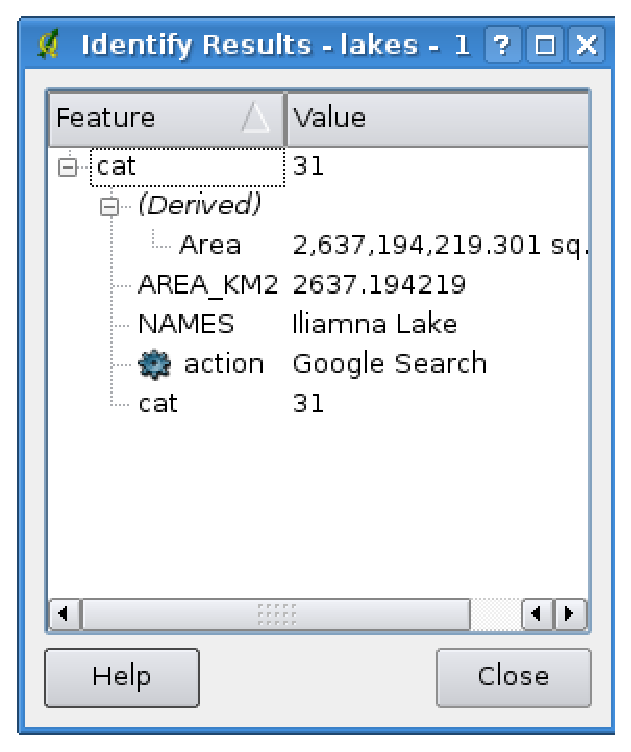
\includegraphics[clip=true, width=8cm]{action_identifyaction} 
\end{center}  
\end{figure}

Cuando hacemos clic en la acci\'on, se abre el Firefox y navega a la URL
\url{http://www.google.com/search?q=Tustumena}. Tambien es posible agregar mas 
campos de atributos a la acci\'on. Por lo tanto puede agregar un ``+'' al final del texto de la acci\'on, 
seleccione otro campo y haga clic en el bot\'on \button{Insert Field}. En este ejemplo no
hay otro campo disponible que tenga sentido que sea b\'uscado.

Puede definir m\'ultiples acciones para una capa y cada una se mostrar\'s en el
di\'alogo \dialog{Identify Results}. Puede tambien invocar acciones desde la tabla de atributos
seleccionando una l\'{\i}nea y haciendo clic, entonces eligiendo la acci\'on desde el men\'u
emergente.

Puede pensar en todos los tipos de usos para las acciones. Por ejemplo, si tiene una capa de puntos
que contenga lugares de im\'agenes o fotos junto con un nombre de archivo, puede
crear una acci\'on para lanzar el visualizador para mostrar la imagen. Tambien puede usar
acciones para lanzar reportes web para un campo de atributos o combinaci\'on de
campos, especificandolos en la misma forma que hicimos con el ejemplo de b\'usqueda en Google.

\subsubsection{Pesta\~na atributos}\index{attributes}\label{label_attributes}
Dentro de la pesta\~na \tab{Attributes} el conjunto de datos seleccionado puede ser manipulado.
Los botones \button{New Column} y \button{Delete Column} pueden ser usados,
cuando el conjunto de datos est\'a en modo de edici\'on. Al momento solo columnas
de capas Postgis pueden ser editados, debido a que esta funcionalidad no es soportada aun 
por la librer\'{\i}a the OGR. 

El bot\'on \button{Toggle editing mode} activa o desactiva este modo.

\minisec{edit widget}

Dentro de la pesta\~na \tab{Attributes} tambien encontrara un \texttt{edit widget} y una columna 
\texttt{value}. Estas dos columnas pueden ser usadas para definir valores o un rango 
de valores que son permitidos agregarse a las columnas de atributos de la tabla especifica. 
Son usadas para producir diferentes widgets de edici\'on en el di\'alogo de atributos. Estos 
widgets son:

\begin{itemize}
\item l\'{\i}nea de edici\'on: un campo de edici\'on que permite capturar texto simple (o restringir a 
n\'umero para atributos n\'umericos).
\item valor \'unico: una lista de atributos \'unicos de las caracter\'{\i}sticas existentes
es generada y presentada en una caja de selecci\'on para su selecci\'on.
\item  valor  \'unico (editable): una combinaci\'on de `l\'{\i}nea de edici\'on' y `valor \'unico'.
El campo de edici\'on completa los valores ingresados a un valor \'unico, pero tambien permite
escribir valores nuevos.
\item mapa de valores: una caja de selecci\'on para seleccionar desde un conjunto de valores especificados en la
columna \texttt{value} de la pesta\~na \tab{Attributes}.  Los posibles valores son 
delimitados por un punto y coma (ej. \verb|high;medium;low|). Tambien es posible
anteponer una etiqueta a cada valor, la cual es delimitada por signo de igual (ej.
\verb|high=1;medium=2;low=3|). La etiqueta se muestra en la caja de selecci\'on en lugar
del valor.
\item clasificaci\'on: si un renderer de valor \'unico es seleccionado para la capa, los valores
usados para las clases son presentados para selecci\'on en una caja de selecci\'on.
\item rango (editable): Un campo de edici\'on que permite restringir valores n\'umericos a un
rango dado.  El rango se especifica capturando un valor m\'{\i}nimo y un valor m\'aximo
delimitado por un punto y coma(ej. \verb|0;360|) en la columna \texttt{value} de
la pesta\~na \tab{Attributes}.
\item rango (slider): Se presenta un widget slider que permite la selecci\'on de un valor
en un rango y precisi\'on dado.  El rango es especificado por valores m\'{\i}nimo, m\'aximo
y un ancho de salto (ej. \verb|0;360;10|) en la columna \texttt{value} de
la pesta\~na \tab{Attributes}.
\item nombre de archivo: un widget de l\'{\i}nea de edici\'on acompa\~nado de un pulsador. Cuando est\'a
presionado permite seleccionar un nombre de archivo usando el di\'alogo de archivo estandar.
\end{itemize}

\subsubsection{Pesta\~na diagrama}\label{sec:diagram}
\index{vector layers!diagram}

La pesta\~na \tab{Diagram} te permite agregar un sobreposici\'on de gr\'aficos a una capa vectorial.
Para activar esta caracter\'{\i}stica, habra al Manejador de Complementos y selecciones el complemento  
de Sobreposici\'on de di\'agramas. Despues de esto, hay una nueva pesta\~na en el di\'alogo de vectores \dialog{Layer
Properties} donde las configuraciones para los diagramas pueden ser capturadas (vea 
la figura~\ref{fig:diagramtab}).

\begin{figure}[ht]
   \begin{center}
   \caption{El di\'alogo de propiedades de vector con la pesta\~na diagramas \nixcaption}\label{fig:diagramtab}\smallskip
   \includegraphics[clip=true, width=13cm]{diagram_tab}
\end{center}
\end{figure}

La implementaci\'on actual de di\'agramas provee soporte para barras, pastel
y para escalado lineal del tama\~no del diagrama de acuerdo a un atributo de
clasificaci\'on. Mostraremos un ejemplo la sobreposici\'on de un gr\'afico de barras
sobre la capa de l\'{\i}mites de Alaska.
Ambas capas vectoriales son parte del conjunto de datos de ejemplo de QGIS (vea
la Secci\'on~\ref{label_sampledata}.

\begin{enumerate}
\item Primero haga clic en el \'{\i}cono \toolbtntwo{mActionAddOgrLayer}{Load Vector},
navegue hasta el directorio con el conjunto de datos de ejemplo de QGIS y cargue las dos capas de vectores
\filename{alaska.shp} y \filename{climate.shp}.
\item Haga doble clic en la capa \filename{climate} en la leyenda del mapa y abra el di\'alogo
\dialog{Layer Properties}.
\item Haga clic en \tab{Diagram Overlay} y seleccione \button{Bar chart} como
tipo de diagrama.
\item En el diagrama necesitamos mostrar los valores de las tres columnas
\filename{T\_F\_JAN, T\_F\_JAN} y \filename{T\_F\_MEAN}. Primero seleccione
\filename{T\_F\_JAN} como atributos y haga clic \button{Add attribute}, entonces
\filename{T\_F\_JUL} y finalemente \filename{T\_F\_MEAN}.  
\item Para escalado lineal del tama\~no del diagrama definimos \filename{T\_F\_JUL}
como atributo de clasificaci\'on.
\item Ahora clic en \button{find maximum value}, elija el tama\~no y unidad y clic
\button{Apply} para mostrar el diagrama en la ventana principal de QGIS.
\item Ahora puede adaptar el tama\~no del gr\'afico, o cambiar los atributos de colores haciendo
doble clic en los valores de colores en el campo atributo.
Figure~\ref{fig:climatediagram} da una impresi\'on.
\item Finalmente haga clic \button{Ok}. 
\end{enumerate}

\begin{figure}[ht]
   \begin{center}
   \caption{Diagrama de datos de temperatura sobrepuesto en un mapa \nixcaption}\label{fig:climatediagram}\smallskip
   \includegraphics[clip=true, width=13cm]{climate_diagram}
\end{center}
\end{figure}

\subsection{Edici\'on}\index{editing}

QGIS suporta capacidades b\'asicas para la edici\'on de geometrias.  Antes de leer mas
deber\'{\i}a notar que en esta etapa el soporte para edici\'on es preliminar.
Antes de realizar cualquier edici\'on, realize siempre una copia de respaldo del conjunto de datos
a editar. 

\textbf{Note} - el procedimiento para editar capas de GRASS es diferente - vea la
Secci\'on \ref{grass_digitising} para detalles.

\subsubsection{Estableciendo la tolerancia del snapping y radio de b\'usqueda}

Antes de poder editar v\'ertices, es muy importante establecer la tolerancia
de snapping y radio de b\'usqueda a valores que permitan una \'optima edici\'on de
las geometr\'{\i}as de capas vectoriales. 

\minisec{Tolerancia de Snapping}

Tolerancia de Snapping es la distancia que QGIS usa para \usertext{search} el v\'ertice
mas cercano y/o segemento al cual tratas de conectar
cuando estableces un nuevo v\'ertice o mueve un v\'ertice existente. If you aren't
within the snap tolerance, QGIS will leave the vertex where you release the
mouse button, instead of snapping it to an existing vertex and/or segment. 

\begin{enumerate}
\item Una tolerancia de snapping general puede ser definida eligiendo
\mainmenuopt{Settings} > \dropmenuopttwo{mActionOptions}{Options}. 
(En Mac: vaya a  \mainmenuopt{QGIS} > Preferencias, en Linux: \mainmenuopt{Edit} > \dropmenuopttwo{mActionOptions}{Options}.)
En la pesta\~na de \tab{Digitizing} puede elegir entre v\'ertice a segmento o v\'ertice a
segmento y v\'ertice como mode de snap por defencto. Tambien puede definir una tolerancia de
snapping por defecto y un radio de b\'usqeuda para edici\'on de v\'ertices. La tolerancia puede ser establecida bien
en unidades de mapa o en pixeles.
En nuestro proyecto de digitalizaci\'on (trabajando con el conjunto de datos de Alaska),
las unidades estas en pies. Sus resultados pueden variar, pero algo en el
orden de 300 pies deber\'{\i}a estar bien a una escala de 1:10 000 y es una configuraci\'on razonable.
\item Una tolerancia de snapping basada en la capa puede ser definida eligiendo
\mainmenuopt{Settings} (or \mainmenuopt{File}) > \dropmenuopttwo{mActionOptions}{Project
Properties\dots}. En la pesta\~na \tab{General}, secci\'on \classname{Digitize} puede hacer clic
en \button{Snapping options\dots} para activar y ajustar el modo de snapping
y tolerancia en una capa (see Figure~\ref{fig:snappingoptions}).
\end{enumerate}

\begin{figure}[H]
   \begin{center}
   \caption{Editar opciones de snapping para una capa \nixcaption}\label{fig:snappingoptions}\smallskip
   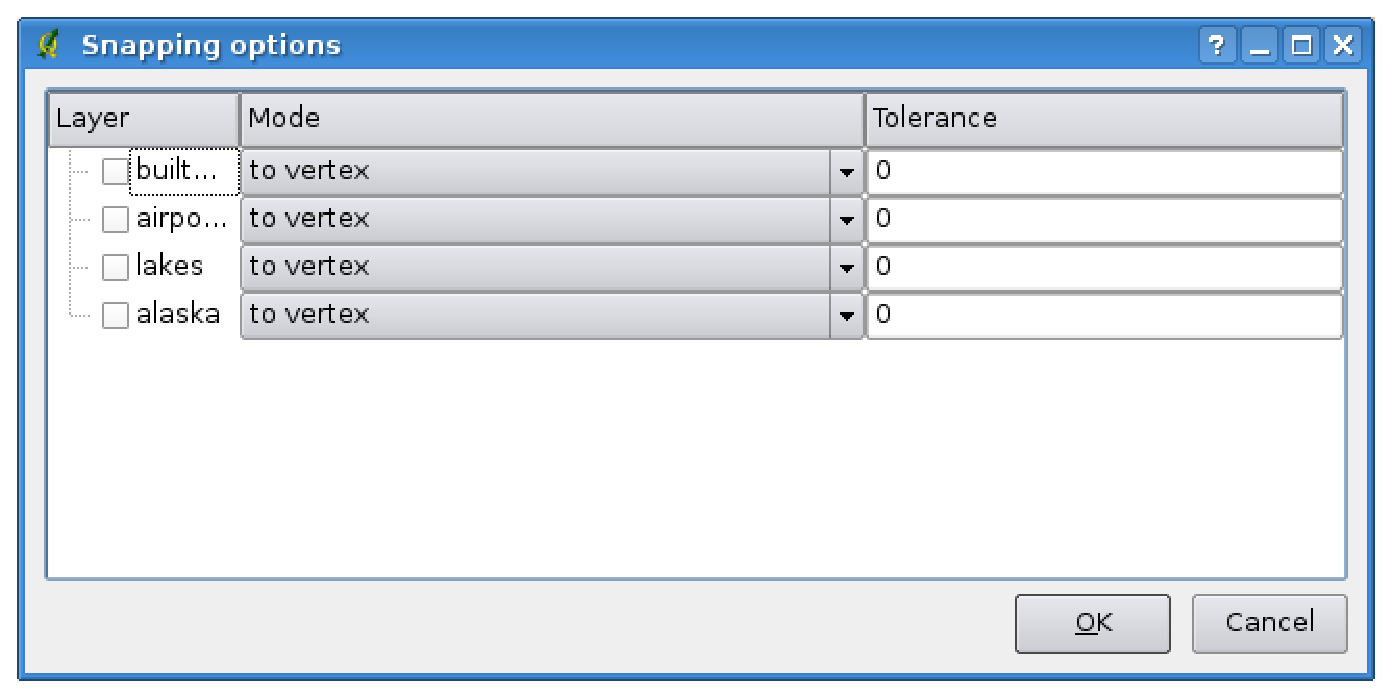
\includegraphics[clip=true, width=14cm]{editProjectSnapping} 
\end{center}  
\end{figure}

\minisec{Radio de b\'usqueda}

El radio de b\'usqueda es la distancia que QGIS usa para \usertext{search} el v\'ertice
mas cercano que se est\'a tratando de mover cuando se hace clic en el
mapa. Si no est\'a dentro del radio de b\'usqueda, QGIS no encontrar\'a y seleccionar\'a
ning\'un v\'ertice para edici\'on y mostrar\'a un molesto mensaje a tal efecto.
La tolerancia de snap tolerance y el radio de b\'usqueda pueden ser establecidos en unidades de mapa o pixeles, de esta manera puede
necesitar experimentar para establecerlos correctamente. Si especifica una tolerancia muy grande
QGIS puede snap al v\'ertice incorrecto, especialmente si est\'a tratando
con un gran n\'umero de v\'ertices muy proximos. Establecer un radio de b\'usqueda muy
peque\~no no encontrar\'a nada a mover.

El radio de b\'usqueda para ediciones de vertices en unidades de capa puede ser definido en la
pesta\~na \tab{Digitizing} bajo \mainmenuopt{Settings} >
\dropmenuopttwo{mActionOptions}{Options}. El mismo lugar donde defini\'o la
tolerancia de snapping general para el proyecto.

\subsubsection{Edici\'on topol\'ogica}

Ademas de las opciones basadas en capa la pesta\~na \tab{General} en el men\'u 
\mainmenuopt{Settings} -> \dropmenuopttwo{mActionOptions}{Project Properties\dots} 
tambien provee algunas funcionalidades topol\'ogicas. 
En el grupo de opciones Digitalizaci\'on puede \checkbox{Activar edici\'on topol\'ogica} y/o activar 
\checkbox{Evitar intersecciones de nuevos pol\'{i}gonos}.

\minisec{Activar edici\'on topol\'ogica}

La opci\'on \checkbox{Activar edici\'on topol\'ogica} es para editar y mantener 
l\'{\i}mites comunes en mosaicos de pol\'{\i}gonos. QGIS "detecta" un l\'{\i}mite compartido en 
un mosaico de pol\'{\i}gonos y solo tiene que mover el v\'ertice una sola vez y QGIS se encargar\'a 
de actualizar el otro l\'{\i}mite.

\minisec{Evitar intersecciones de nuevos pol\'{\i}gonos}

La segunda opci\'on topol\'ogica llamada \checkbox{Evitar intersecci\'on de nuevos pol\'{\i}gonos} 
evita traslapes en mosaicos de pol\'{\i}gonos. Es para digitalizaci\'on r\'apida de pol\'{\i}gonos adyacentes. 
Si ya tiene un pol\'{\i}gono, es posible con esta opci\'on digitalizar la segunda 
de tal forma que las dos se intersecten y Qgis entonces corta el segundo pol\'{i}gono en el l\'{i}mite com\'un. 
La ventaja es que los usuarios no tienen que digitalizar todos los v\'ertices del l\'{i}mite com\'un.

\subsubsection{Edici\'on de una capa existente}
\index{vector layers!editing}
\index{editing!an existing layer}
\label{sec:edit_existing_layer}

Por defecto, QGIS carga capas como solo lectura: Esto es una medida de seguridad
para evitar editar accidentalmente una capa si hay un dezlis del mouse.
Sin embargo, puede elegir editar una capa siempre y cuando el proveedor de datos lo soporte,
y el conjunto de datos sea escribible (ej. sus archivos no son de solo escritura).

La edici\'on de capas es mas versatil cuando es usada en conjuntos de datos PostgreSQL/PostGIS. 

\begin{Tip}[ht]\caption{\textsc{Integridad de datos}}
\qgistip{Siempre es una buena idea respaldar su conjunto de datos antes de iniciar 
la edici\'on. Mientras los autores de QGIS han realizado cada esfuerzo para preservar 
la integridad de sus datos, no se ofrece garant\'{\i}a en este aspecto.
}
\end{Tip}

\begin{Tip}[ht]\caption{\textsc{Manipulando datos de atributos}}
\qgistip{Actualmente solo capas de PostGIS son soportadas para agregar y eliminar columnas de atributos
dentro de este di\'alogo. En versiones futuras de QGIS, otros conjuntos de datos ser\'an soportados, 
porque esta funcionalidad fue recientemente implementada en GDAL/OGR > 1.6.0
}
\end{Tip}



\begin{Tip}[ht]\caption{\textsc{Guarde regularmente}}
\qgistip{Recuerde desactivar \toolbtntwo{mActionToggleEditing}{Toggle editing} regularmente.  
Esto le permite guardar los cambios recientes,
y tambien confirmar que los conjuntos de datos pueden aceptar todos los cambios.
}
\end{Tip}

\begin{Tip}[ht]\caption{\textsc{Ediciones concurrentes}}
\qgistip{Esta versi\'on de QGIS no rastrea si alguien mas est\'a editando una caracter\'{i}stica al mismo tiempo
que usted.  La \'ultima persona en guardar su edici\'on gana.
}
\end{Tip}

\begin{Tip}[ht]\caption{\textsc{Haga un acercamiento antes de empezar a editar}}
\qgistip{Antes de editar una capa, deber\'{\i}a hacer un acercamiento
a su \'area de inter\'es. Esto evita esperar mientras los marcadores de v\'ertices 
son dibujados en la capa completa.
}
\end{Tip}

\begin{Tip}[ht]\caption{\textsc{Marcadores de v\'ertices}}
\qgistip{
La versi\'on actual de QGIS soporta dos tipos de marcadores de v\'ertices 
un c\'irculo semi-transparente o una cruz. Para cambiar el estilo de marcador, elija
\dropmenuopttwo{mActionOptions}{Options} del men\'u
\mainmenuopt{Settings} y haga clic en la pesta\~na \tab{Digitizing} y selecciones
la entrada apropiada.
}
\end{Tip}

Todas las sesiones de edici\'on comienzan eligiendo la opci\'on \dropmenuopttwo{mActionToggleEditing}{Toggle editing}.
Esta puede ser encontrada en el men\'u contextual haciendo clic derecho en la entrada para esa capa en la leyenda.
\index{Allow Editing}
Alternativamente, puede usar el bot\'on \index{Toggle Editing}
\toolbtntwo{mActionToggleEditing}{Toggle editing} de la barra de herramientas para empezar o parar 
el modo de edici\'on.\index{editing!icons} Una vez que la capa est\'a en modo de edic\'on, 
los marcadores aparecer\'an en los v\'ertices, y botones adicionales en la barra de herramientas 
estar\'an disponibles.

\minisec{Haciendo zoom y pan con la rueda del rat\'on}

Mientras esta digitalizando puede presionar la rueda del rat\'on para hacer un pan dentro de la ventana
principal y puede girar la rueda para acercarse o alejarse en el mapa. Para alejarse
posicione el cursor del rat\'on dentro del \'area del mapa y gire hacia atras (hacia usted) 
para acercarse gire la rueda del rat\'on hacia afuera (alejandose de usted). La posici\'on del cursor del mouse ser\'a el centro 
del zoom al \'area de inter\'es. Puede personalizar el comportamiento 
de la rueda del mouse usando la pesta\~na \tab{Map tools} bajo el men\'u
\mainmenuopt{Settings} >\dropmenuopt{Options}.  

\minisec{Desplazamiento con las teclas de flechas}

Es posible desplazar el mapa  durante la digitalizaci\'on con las teclas de flecha. Posicione
el cursor del mouse dentro del \'area de mapa presione la flecha derecha para hacer un
desplazamiento al este, tecla de flecha izquierda para desplazarse al oeste, tecla de flecha hacia arriba para desplazarse al norte y flecha hacia abajo 
para desplazarse al sur.

Tambien puede usar la barra espaciadora para temporalmente causar movimientos del mouse para hacer desplazamientos 
al mapa. Las teclas PgUp y PgDown en su teclado causar\'an que la vista se acerque 
o aleje sin interrumpir su sesi\'on de digitalizaci\'on.

You can perform the following editing functions:

\begin{itemize}
\item Add Features: \toolbtntwo{mActionCapturePoint}{Capturar Punto},
  \toolbtntwo{mActionCaptureLine}{Capturar L\'{\i}nea} y
  \toolbtntwo{mActionCapturePolygon}{Capturar Pol\'{\i}gono}
\item \toolbtntwo{mActionAddRing}{Agregar Anillo}
\item \toolbtntwo{mActionAddIsland}{Agregar Isla}
\item \toolbtntwo{mActionSplitFeatures}{Partir Caracter\'{\i}sticas}
\item \toolbtntwo{mActionMoveFeature}{Mover Caracter\'{\i}sticas}
\item \toolbtntwo{mActionMoveVertex}{Mover V\'ertice}
\item \toolbtntwo{mActionAddVertex}{Agregar V\'ertice}
\item \toolbtntwo{mActionDeleteVertex}{Eliminar V\'ertice}
\item \toolbtntwo{mActionDeleteSelected}{Eliminar Seleccionado}
\item \toolbtntwo{mActionEditCut}{Cortar Caracter\'{\i}sticas}
\item \toolbtntwo{mActionEditCopy}{Copiar Caracter\'{\i}sticas}
\item \toolbtntwo{mActionEditPaste}{Pegar Caracter\'{\i}sticas}
\end{itemize}

\minisec{Agregando Caracter\'{\i}sticas}
\index{vector layers!adding!feature}

Antes de iniciar agregando caracter\'{\i}sticas, use las herramientas \toolbtntwo{mActionPan}{pan}
y \toolbtntwo{mActionZoomIn}{zoom-in}/\toolbtntwo{mActionZoomOut}{zoom-out} 
para navegar al \'area de inter\'es.

Entonces puede usar los \'{\i}conos \toolbtntwo{mActionCapturePoint}{Capturar punto},
\toolbtntwo{mActionCaptureLine}{Capture l\'{\i}nea} o
\toolbtntwo{mActionCapturePolygon}{Capturar pol\'{\i}gono} en la barra de herramientas para poner el cursor de QGIS
en modo de digitalizaci\'on.

Para cada caracter\'{\i}sticas, primero digitaliza la geometr\'{\i}a, despues captura sus atributos.

Para digitalizar la geometr\'{\i}a, haga clic izquierdo en el \'area del mapa para crear el primer
punto de su nueva caracter\'{\i}stica.

Para l\'{\i}neas y pol\'{\i}gonos, siga haciendo clic izquierdo para cada punto adicional
que desee capturar. Cuando haya finalizado de agregar puntos,
haga clic derecho en cualquier parte del \'area de mapa para confirmar que ha terminados de meter
la geometr\'{i}a de esa caracter\'{\i}stica.

La ventana de atributos aparecer\'a, permitiendole meter la informaci\'on de la nueva caracter\'{\i}stica.
Figure \ref{fig:vector_digitising} muestra como establecer atributos para un nuevo rio ficticio
en Alaska.

\begin{figure}[ht]
   \begin{center}
   \caption{Di\'alogo de Captura de Atributos despues de digitalizar una nueva caracter\'{\i}stica vectorial
   \nixcaption}\label{fig:vector_digitising}\smallskip
   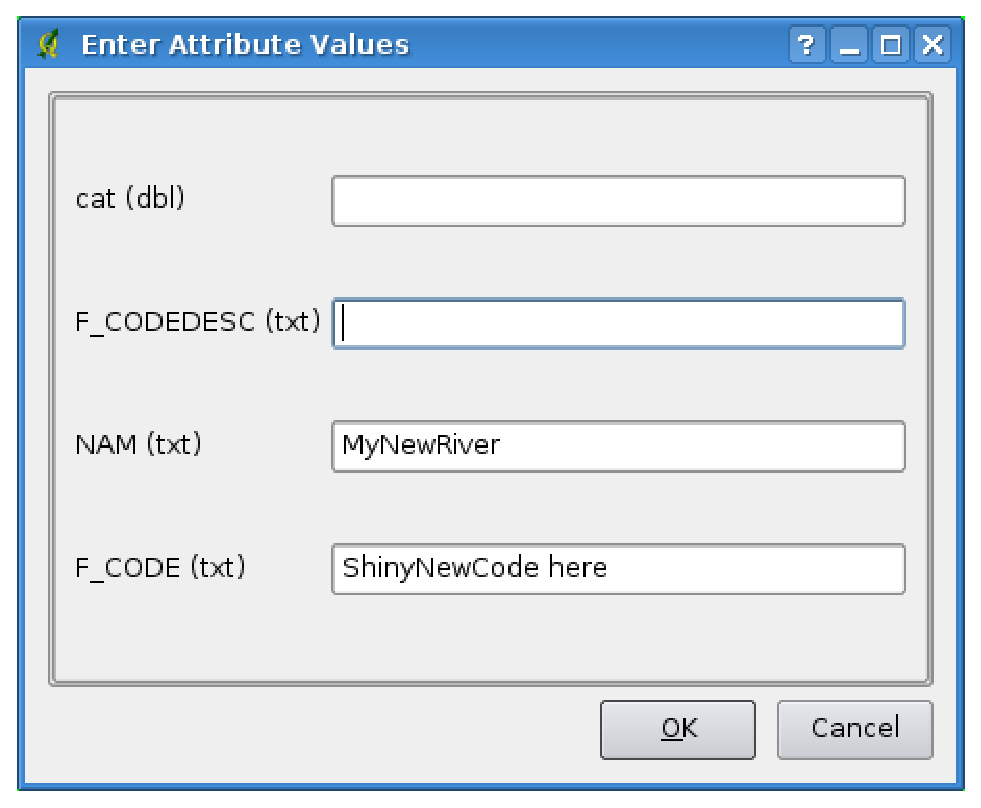
\includegraphics[clip=true, width=8cm]{editDigitizing}
\end{center}  
\end{figure}

\begin{Tip}[ht]\caption{\textsc{Tipos de Valores de Atributos}}
\qgistip{
Al menos para edici\'on de shapefiles los tipos de atributos son validados durante la
captura. Por esto, no es posible capturar un n\'umero dentro de una columna de texto en el di\'alogo
\dialog{Capturar Valores de Atributos} o viceversa. Si necesita hacerlo as\'{\i},
deber\'{\i}a editar los atributos en un segundo paso dentro del di\'alogo \dialog{Attribute
table}.
}
\end{Tip}

\minisec{Mover Caracter\'{\i}stica}
\index{vector layers!move!feature}

Puede mover caracter\'{\i}sticas usando el \'{\i}cono \toolbtntwo{mActionMoveFeature}{Move Feature} 
de la barra de herramientas.

\minisec{Partir Caracter\'{\i}stica}
\index{vector layers!split!feature}

Puede partir caracter\'{\i}sticas usando el \'{\i}cono \toolbtntwo{mActionSplitFeatures}{Split Features}
de la barra de herramientas.

\minisec{Editando V\'ertices de una Caracter\'{\i}stica}
\index{vector layers!editing!vertex}

Para ambos tipos de capas PostgreSQL/PostGIS y  shapefile, los v\'ertices de las caracter\'{\i}sticas pueden ser editados. 

Los v\'ertices pueden ser directamente editados, esto es, no tiene
que elegir cual nueva caracter\'{\i}stica editar antes de que pueda cambiar
su geometr\'{\i}a.
En algunos casos, m\'ultiples caracter\'{\i}sticas pueden compartir el mismo v\'ertice
y de esta manera los siguientes reglas aplican cuando el mouse es presionado
cerca de caracter\'{\i}sticas del mapa:

\begin{itemize}
\item \textbf{L\'{\i}neas}    - La l{\'i}nea mas cercana a la posici\'on del rat\'on
                          es usada como caracter\'{\i}stica objetivo.
                          Entonces (para mover y eliminar un v\'ertice)
                          el v\'ertice mas cercano
                          en esa l\'{\i}nea es el objetivo de edici\'on.

\item \textbf{Pol\'{\i}gonos} - Si el rat\'on est\'a dentro del pol\'{\i}gono, entonces este
                          es la caracter\'{\i}stica objetivo; de lo contrario el pol\'{\i}gono mas cercano
                          es usado.
                          Entonces (para mover y eliminar un v\'ertice)
                          el v\'ertice mas cercano
                          en ese pol\'{\i}gono es el objetivo de edici\'on.                          
\end{itemize}

Necesitar\'a establecer la propiedad
\mainmenuopt{Settings}>\dropmenuopttwo{mActionOptions}{Options}>\tab{Digitalizando}>\selectnumber{Radio de b\'usqueda}{10}
a un n\'umero mayor que cero.  De lo contrario QGIS no podr\'a decir que caracter\'{\i}stica esta siendo editeda.


\minisec{Agregando V\'ertices de una Caracter\'{\i}stica}
\index{vector layers!adding!vertex}

Puede agregar nuevos v\'ertices a una caracter\'{\i}stica usando el \'{\i}cono
\toolbtntwo{mActionAddVertex}{Add Vertex} 
de la barra de herramientas.

Note que, no tiene sentido agregar mas v\'ertices a una caracter\'{\i}stica de punto!

En esta versi\'on de QGIS, los v\'ertices solo pueden ser agregados a un \textit{existing} segmento
de una caracter\'{\i}stica de l\'{\i}nea.  Si quieres extender una l\'{\i}nea mas all\'a de su final,
necesitaras primero mover el v\'ertice final, entonces agrega un nuevo v\'ertice donde
el terminal solia estar.

\minisec{Moviendo V\'ertices de una Caracter\'{\i}stica}
\index{vector layers!moving!vertex}

Puede mover v\'ertices usando el \'{\i}cono \toolbtntwo{mActionMoveVertex}{Mover V\'ertice}
de la barra de herramientas.

\minisec{Eliminando V\'ertices de una Caracter\'{\i}stica}
\index{vector layers!deleting!vertex}

Puede eliminar v\'ertices usando el \'{\i}cono \toolbtntwo{mActionDeleteVertex}{Delete Vertex}
de la barra de herramientas.

Note que, no tiene sentido eliminar el v\'ertice de una caracter\'{\i}stica de Punto!
En lugar de eso elimine la caracter\'{\i}stica completa.

Similarment, una l\'{\i}nea de un solo v\'ertice o pol\'{\i}gono de dos v\'ertices tambien es
bastante inutil y llevar\'a a resultados impredecibles en alg\'un otro lugar
QGIS, as\'{\i} que no lo haga.

\textbf{advertencia:} Un v\'ertice es identificado para eliminaci\'on tan pronto 
como haces clic con el rat\'on cerca de una caracter\'{\i}stica elegible.
Para deshacer, necesitaras desactivar
la edici\'on y despues descartar sus cambios.
(Claro esto significar\'a que otros cambios sin guardar ser\'an perdidos, tambien.)

\minisec{Agregar Anillo}
\index{vector layers!add!ring}

Puede crear pol\'{\i}gonos anillo usando el \'{\i}cono \toolbtntwo{mActionAddRing}{Add Ring}
de la barra de herramientas. Esto significa que dentro de un \'area existente es posible digitalizar
otros pol\'{\i}gonos, esto ocurrir\'a como un 'todo', de esta manera solo 
el \'area entre los l\'{\i}mites del pol\'{\i}gono mas externo y el mas interno permanecen 
como un pol\'{\i}gono de anillo. 

\minisec{Agregar Isla}
\index{vector layers!add!island}

Puede \toolbtntwo{mActionAddIsland}{agregar isla} a seleccionados multipol\'{\i}gonos. 
El nuevo pol\'{\i}gono isla tiene que ser digitalizado fuera del multipol\'{\i}gono seleccionado. 

\minisec{Cortando, Copiando y Pegando Caracter\'{\i}sticas}
\index{vector layers!cut!feature}
\index{vector layers!copy!feature}
\index{vector layers!paste!feature}
\index{editing!cutting features}
\index{editing!copying features}
\index{editing!pasting features}

Las caracter\'{\i}sticas seleccionadas pueden ser cortadas, copiadas y pegadas entre capas en el mismo proyecto
de QGIS, siempre y cuado de antemano las capas de destino han sido establecidas a 
\toolbtntwo{mActionToggleEditing}{Activar edici\'on}.

Las caracter\'{\i}stica pueden tambien ser pegadas a aplicaciones externas como texto:  Esto es,
las caracter\'{\i}sticas son presentadas en formato CSV con los datos de geometr\'{\i}a 
en el formtado Well-Known Text (WKT) de la OGC.


Sin embargo en esta version de QGIS, texto de caracter\'{\i}sticas de fuera de QGIS no pueden 
ser pegadas a una capa dentro de QGIS. ?`Cuando seria \'util la funci\'on de copiar y pegar? 
Bien, resulta que puede editar mas de una capa 
al tiempo que copia y pega caracter\'{\i}sticas entre capas. ?`Por qu\'e querriamos hacer
eso?  dicho que tenemos que hacer una trabajo sobre una nueva capa pero solo necesita uno o
dos lagos, no los 5,000 en nuestra capa \filename{big\_lakes}. Podemos crear una nueva capa
y usar copiar/pegar para soltar los lagos necesarios en ella. 

Como un ejemplo estamos copiando algunos lagos a una nueva capa:

\begin{enumerate}
\item Cargue la capa de la que desea copiar (capa fuente)
\item Cargue o cree la capa a la que desea copiar (capa destino) 
\item Inicie la edici\'on para la capa destino
\item Haga la capa fuente activa haciendo clic en ella en la leyenda 
\item Use la herramienta \toolbtntwo{mActionSelect}{Seleccionar} para seleccionar la caracter\'{\i}sticas(s) en la capa fuente
\item Haga clic en la herramienta \toolbtntwo{mActionEditCopy}{Copy Features}
\item Haga la capa destibo activa haciendo clic en ella en la leyenda 
\item Haga clic en la herramienta \toolbtntwo{mActionEditPaste}{Paste Features}
\item Pare la edici\'on y guarde los cambios
\end{enumerate}

?`Qu\'e pasa si las capas fuentes y destino tienen
diferentes esquemas (no son iguales los nombres de campos y tipos)? QGIS llena
lo que coincide e ignora el resto. Si no le interesa los atributos
siendo copiados a la capa destino, no importa como dise\~ne los
campos y los tipos de datos. Si desea asegurarse que todo - caracter\'{\i}sticas y sus
atributos - son copiados, aseg\'urese que los esquemas coincidan.

\begin{Tip}[ht]\caption{\textsc{Congruencia de Caracter\'{\i}sticas Pegadas}}
\qgistip{Si sus capas de fuente y destino usan la 
misma proyecc\'on, entonces las caracter\'{\i}sticas pegadas tendr\'an
una geometr\'{\i}a id\'entica a la capa fuente.
Sin embargo si la capa destino tiene una proyecci\'on diferente
entonces QGIS no puede garantizar que la geometr\'{\i}a es identica.
Esto es simplemente porque hay peque\~nos errores de redondeo
envolucrados durante la conversi\'on entre proyecciones.
}
\end{Tip}

\minisec{Eliminado Caracter\'{\i}sticas Seleccionadas}
\index{vector layers!deleting!feature}

Si deseamos eliminar un pol\'{\i}gono completo, podemos hacerlo primero seleccionando 
el pol\'{\i}gono usando la herramienta regurla \toolbtntwo{mActionSelect}{Select Features}. Puede seleccionar 
m\'ultiples caracter\'{\i}sticas para su eliminaci\'on. Una vez que ha establecido la selecci\'on, use la 
herramienta \toolbtntwo{mActionDeleteSelected}{Eliminar Seleccionado} para eliminar las caracter\'{\i}sticas. No hay funci\'on deshacer, 
pero recuerde que su capa no ha cambiado realmente hasta que pare la edici\'on y elija 
guardar los cambios. De esta manera si comete alg\'un error, siempre puede cancelar el guardado.

La herramienta \toolbtntwo{mActionEditCut}{Cortar Caracter\'{\i}sticas} en la barra de herramientas de digitalizaci\'on puede
tambien ser usada para eliminar caracter\'{\i}sticas. Esto efectivamente elimina la caracter\'{\i}sticas pero
tambien la coloca en un lugar especial llamado ``portapapeles espacial". De esta manera cortamos la caracter\'{\i}stica a eliminar. 
Podemos entonces usar la \toolbtntwo{mActionEditPaste}{herramienta pegar} para regresarla, d\'andonos un deshacer de un nivel 
capability. Cut, copy, and paste work on the currently selected features, 
significando que podemos operar en mas de una al mismo tiempo.

\begin{Tip}[ht]\caption{\textsc{Soporte para la Eliminaci\'on de Caracter\'{\i}sticas}}
\qgistip{Cuando se edita ESRI shapefiles, el borrado
de caracter\'{\i}sticas solo trabaja si QGIS est\'a compilado con una versi\'on de GDAL version 1.3.2 o mayor. 
Las versiones de OS X y Windows QGIS disponibles en el sitio de descarga estan compilados 
usando GDAL 1.3.2 o mayor.
}
\end{Tip}

\minisec{Modo Snap}
\index{editing!snap}
QGIS permite que los v\'ertices digitalizados sean snapped a otros v\'ertices de la misma capa. Para 
establecer la tolerancia de snapping, vaya a
\mainmenuopt{Settings}>\dropmenuopttwo{mActionOptions}{Options}->\tab{Digitizing}.
(En Mac: vaya a  \mainmenuopt{QGIS} > Preferencias, En Linux: \mainmenuopt{Edit} > \dropmenuopttwo{mActionOptions}{Options}.)
Note que la tolerancia de snapping est\'a en unidades de mapa o pixeles.

\minisec{Guardadno Capas Editadas}
\index{editing!saving changes}

Cuando una capa est\'a en modo de edici\'on, cualquier cambio permanece pendiente en la memoria de QGIS.
Por lo tanto no se guardan o se les aplica un commit inmediatamente al conjunto de datos o disco.
Cuando desactiva la edici\'on (o sale de QGIS para el caso), 
se le pregunta si desea guardar sus cambios o
descartarlos.

Si los cambios no pueden ser guardados (ej. disco lleno, o los atributos tienen
valores fuera de rango), el estado de memoria de QGIS es preservado.  Esto
permites que ajuste su edici\'on y lo intente de nuevo.

\subsubsection{Creando una nueva capa}\label{sec:create shape}\index{editing!creating a new layer}

Para crear una nueva capa para edici\'on, elija \toolbtntwo{mActionNewVectorLayer}{New Vector Layer} del
\mainmenuopt{Layer} men\'u. 
Se mostrar\'a un dia\'alogo \dialog{New Vector Layer} como el de la
Figura \ref{fig:newvectorlayer}. Elija el tipo de capa (point,
line o polygon).

\begin{figure}[ht]
   \begin{center}
   \caption{Di\'alogo creando una nueva capa \nixcaption}\label{fig:newvectorlayer}\smallskip
   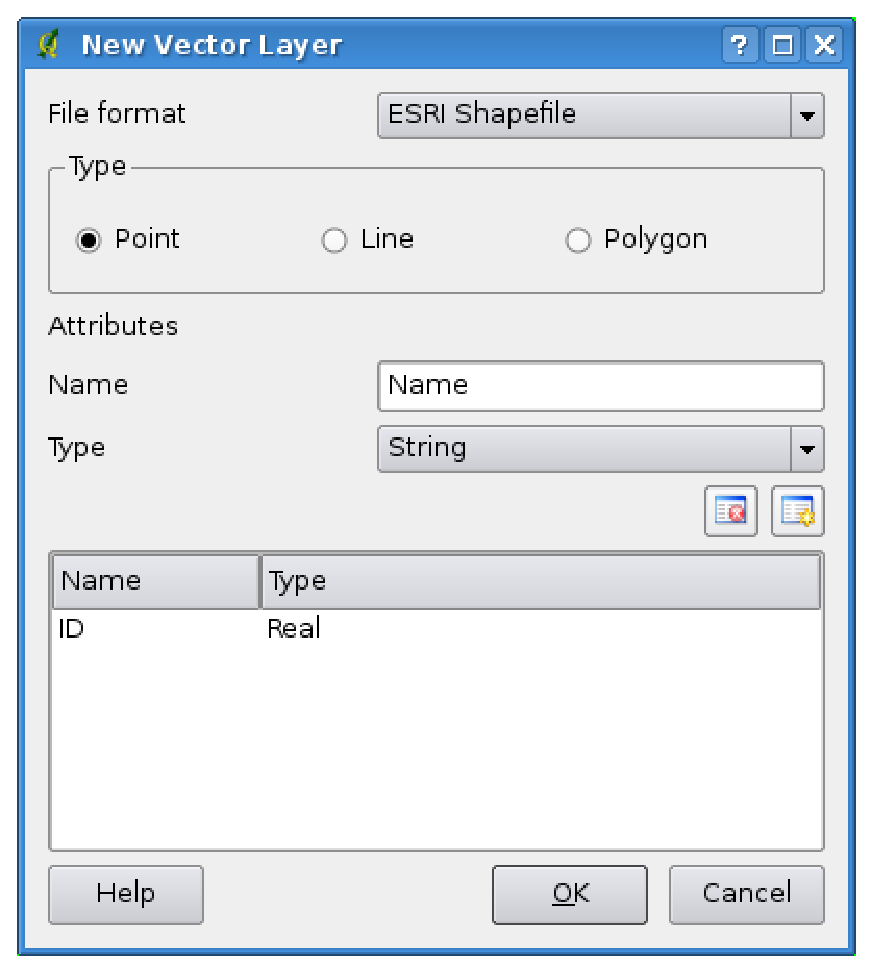
\includegraphics[clip=true, width=10cm]{editNewVector}
\end{center} 
\end{figure}

Note que QGIS no soporta aun la creaci\'on de
caracter\'{\i}sticas 2.5D (ej. caracter\'{\i}sticas con coordenadas X,Y,Z) o caracter\'{\i}sticas de medidas.
A la fecha solo pueden ser creados shapefiles. En una futura versi\'on de QGIS, la creaci\'on de cualquier tipo
de capa OGR o PostgreSQL ser\'a soportado. 

La creaci\'on de capas GRASS es soportada dentro del complemento de GRASS. Vea la secci\'on 
\ref{sec:creating_new_grass_vectors} para mas informaci\'on de creaci\'on de capas GRASS.

Para completar la creaci\'on de una nueva capa, agregue los atributos deseados haciendo
clic en el bot\'on  \button{Add} y especificando un campo y el tipo para al atributo.
Solo los tipos de atributos \selectstring{Type}{real}, \selectstring{Type}{integer}, y \selectstring{Type}{string} son soportados. Una vez que esta contento con sus atributos,
haga clic en \button{OK} y provea un nombre para el shapefile.
QGIS autom\'aticamente agregar\'a una extensi\'on \filename{.shp} al nombre que especific\'o. Una vez
que la capa ha sido creada, ser\'a agregada al mapa y puede ser editada en la misma forma
que se describe en la Secci\'on anterior \ref{sec:edit_existing_layer}. 

\subsubsection{Trabajando con la tabla de atributos}\label{sec:attribute table}\index{editing!working with the attribute table}

Para abrir la tabla de atributos para una capa vectorial, haga la capa activa haciendo clic en ella en el \'area de leyenda del mapa. 
Entonces use el men\'u  capa\mainmenuopt{Layer} del men\'u principal y elija \dropmenuopttwo{mActionOpenTable}{Open Attribute Table} 
desde el men\'u. Tambien es posible hacer clic derechi en la capa y elegir \dropmenuopttwo{mActionOpenTable}{Open Attribute Table} 
desde el men\'u desplegable. Esto abrir\'a una nueva ventana que mostrar\'a los atributos para cada caracter\'{\i}stica en la capa 
(figure \ref{fig:attributetable}).

\begin{figure}[ht]
   \begin{center}
   \caption{Tabla de atributos para la tabla de Alaska \nixcaption}\label{fig:attributetable}\smallskip
   \includegraphics[clip=true, width=12cm]{vectorAttributeTable}
\end{center} 
\end{figure}

Cada columna puede ser ordenada haciendo clic en su encabezado. Una peque\~na flecha indica el orden 
(apuntando hacia abajo significa valores descendentes de la primara columna hacia abajo, apuntando hacia arriba significa valores ascendentes desde la primera columna hacia abajo). 
Para una selecci\'on simple de atributos en una columna el bot\'on \button{Look for} 
puede ser usado. Seleccione el campo (columna) en la cual la b\'usqueda ser\'a realizada 
el men\'u desplegable y presione el bot\'on \button{Search}. Para b\'usquedas mas complejas use
el bot\'on B\'usquedas Avanzadas \button{...}, el cual lanzar\'a el Constructor de Consultas de B\'usqueda descrito en 
la Secci\'on \ref{sec:select_by_query}. 

Para solo mostrar los registros, use la caja de selecci\'on \checkbox{Show selected records only}.
Usando los botones en la parte izquierda inferior de la ventana, seleccione los campos que ser\'an removidos, 
movidos a la parte superior de la tabla, o la selecci\'on que ser\'a invertida. Las caracter\'{\i}sticas seleccionadas pueden ser movidas, copiadas al portapapeles, tambien puede ser hecho con \keystroke{Ctrl-C}. Puede hacer zoom 
a las caracter\'{\i}sticas seleccionadas en el mapa. Activando la edici\'on permite editar valores de atributos. 

\subsection{Constructor de consultas}\label{sec:query_builder}
\index{Query Builder}

El Constructor de Consultas permite definir un conjunto de una tabla y mostrarlo como una capa en QGIS. Actualmente solo puede ser usado con capas PostGIS. 
Por ejemplo, si se tiene una capa \filename{towns} con un campo \usertext{population} se puede seleccionar solo ciudades grandes escribiendo \usertext{population > 100000} en la caja SQL del constructor de consultas. Figura
\ref{fig:query_builder} muestra un ejemplo del constructor de consultas llenado con datos de una capa PostGIS con atributos almacenada en PostgreSQL. 

\begin{figure}[ht]
  \begin{center}
    \caption{Query Builder \nixcaption}\label{fig:query_builder}\smallskip
    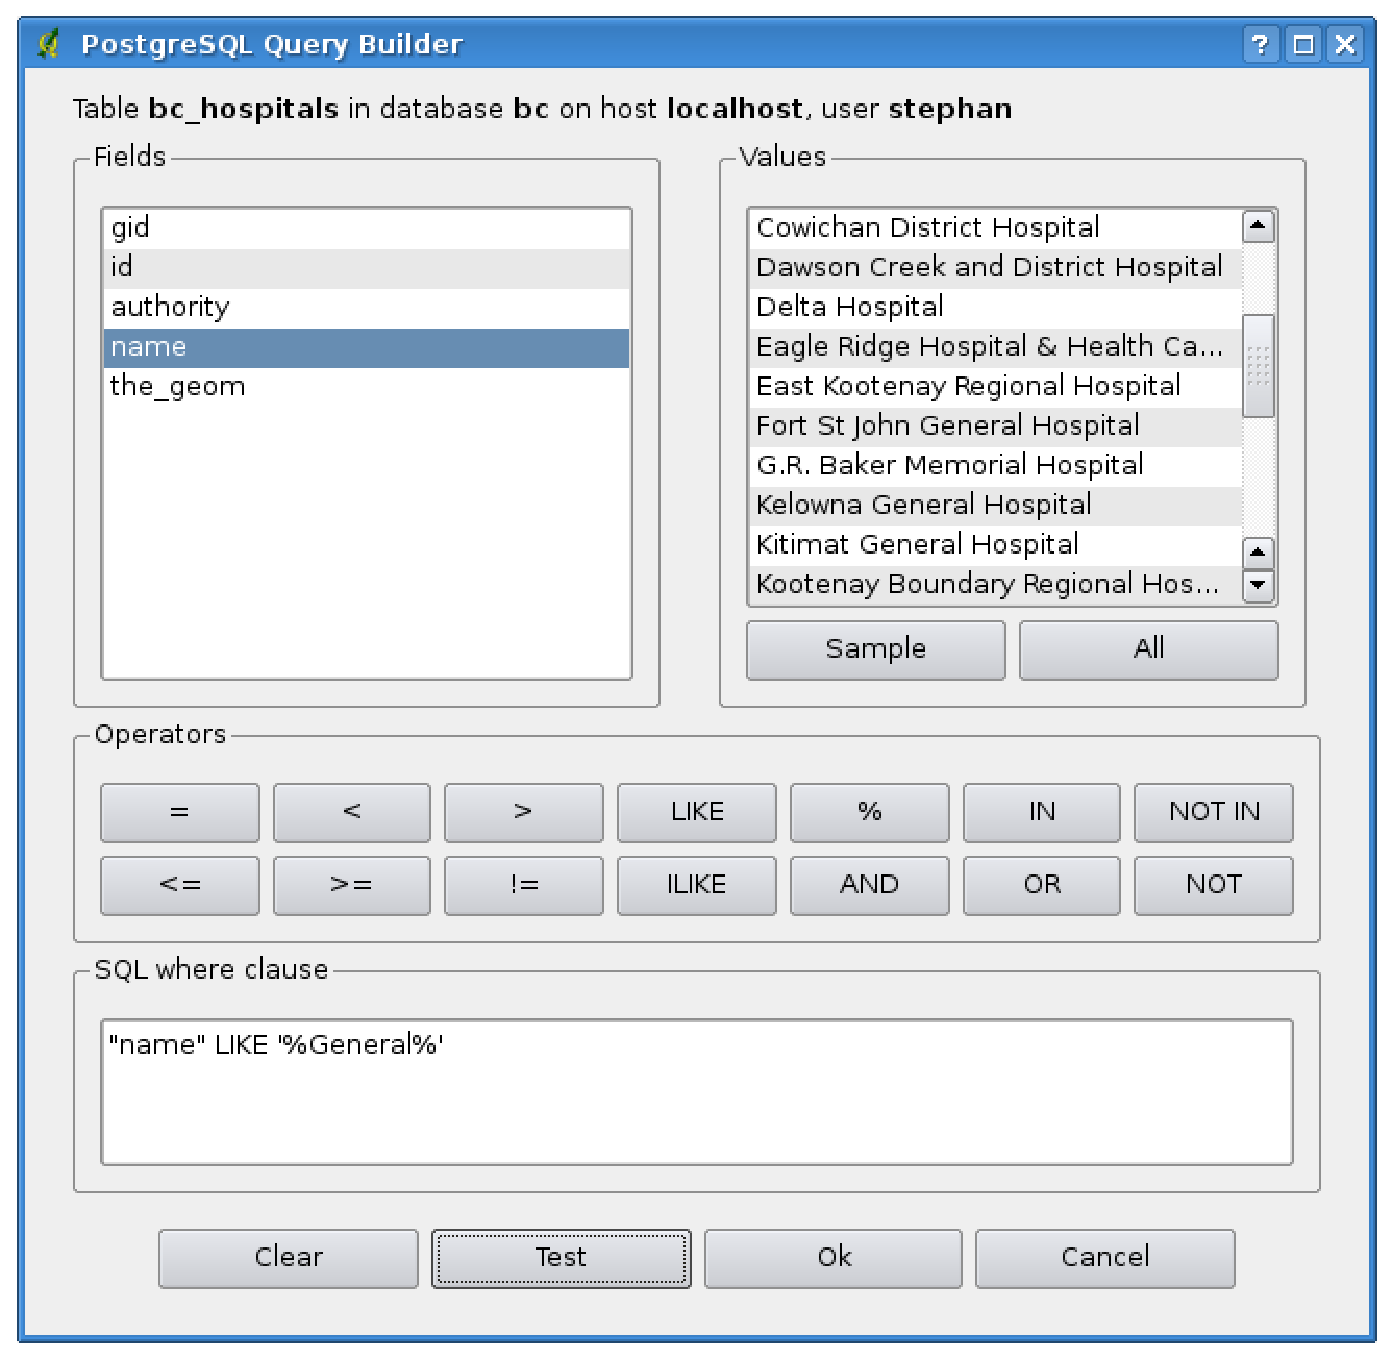
\includegraphics[clip=true, width=11.5cm]{queryBuilder}
  \end{center}  
\end{figure}

El constructor de consultas \index{Query Builder} muestra los campos de la capa de la base de datos en una lista en la izquierda. Puede obtener un ejemplo de los datos contenidos en el campo resaltado haciendo clic en el bot\'on \button{Sample} \index{Query
Builder!generating sample list}. Esto recupera los primeros 25 valores distintos para el campo desde la base de datos. Para obtener una lista de todos los posibles valores para un campo, haga clic en el bot\'onf \button{All} \index{Query Builder!getting all
values}. Para agregar un campo seleccionado o valor a la consulta, haga doble clic en el\index{Query Builder!adding fields}. Puede usar varios botones para construir la consulta o puede escribirla dentro de la caja SQL.

Para probar una consulta, haga clic en el bot\'on \button{Test} \index{Query Builder!testing
queries}. Esto regresar\'a un conteo del n\'umero de registros que pueden ser incluidos en la capa. Cuando est\'e satisfecho con la consulta, haga click en el bot\'on \button{OK}. El SQL para la clausula where ser\'a mostrada en la columna SQL de la lista de capas.

\begin{Tip}\caption{\textsc{Changing the Layer Definition}}\index{Query
Builder!changing layer definitions}
\qgistip{You can change the layer definition after it is loaded by altering
the SQL query used to define the layer. To do this, open the 
vector \dialog{Layer Properties} dialog by double-clicking on the layer in the legend and click on the
\button{Query Builder} button on the \tab{General} tab. See Section
\ref{sec:vectorprops} for more information.}
\end{Tip}

\subsection{Selecci\'on por consulta}\label{sec:select_by_query}
\index{PostgreSQL!query builder}
\index{PostGIS!query builder}
\index{query builder!PostgreSQL}
\index{query builder!PostGIS}

Con QGIS es tambien posible seleccionar caracter\'isticas usando una interface similar al constructor de consultas utilizado en \ref{sec:query_builder}. En la secci\'on superior el proposito el prop\'osito del constructor de consultas es solo mostrar las caracter\'{\i}sticas cumpliendo el filtro de ser un subconjunto de una 'capa virtual'. El prop\'osito de la funci\'on de consulta seleccionar por es la de resaltar todas las caracter\'{\i}sticas que cumplan con un criterio particular. Seleccionar por consulta puede ser usado con todos los complementos proveedores de datos.

Para hacer una 'selecci\'on por consulta' en una capa cargada, haga clic en el bot\'on \toolbtntwo{mActionOpenTable}{Open Table} para abrir la tabla de atributos de la capa. Entonces clic en el bot\'on \button{Advanced...} en la parte inferior. Esto inicia el Constructor de Consultas que permite definir un subconjunto de una tabla y mostrarlo como se describe en la Secci\'on \ref{sec:query_builder}.


\index{vector layers|)}

% vim: set textwidth=78 autoindent:

% \section{Working with Raster Data}\label{label_raster}
\section{Travailler sur des donn\'ees raster}\label{label_raster}
\index{couches raster|(}

% when the revision of a section has been finalized, 
% comment out the following line:
%\updatedisclaimer

% This Section describes how to visualize and set raster layer properties.
% QGIS supports a number of different raster formats. Currently tested formats
% include:\index{raster layers!data formats}
Cette section explique comment visualiser et d\'efinir les propri\'et\'es d'une couche
raster. QGIS g\`ere diff\'erents formats raster. Aujourd'hui les formats test\'es
incluent :\index{couches raster!formats de donn\'ees}
\begin{itemize}
\item Arc/Info Binary Grid
\item Arc/Info ASCII Grid
\item Raster GRASS
\item GeoTIFF
\item JPEG
\item Spatial Data Transfer Standard Grids (avec quelques limitations)
\item DEM ASCII de l'USGS
\item Erdas Imagine
\end{itemize}

% Because the raster implementation in QGIS is based on the GDAL library, other
% raster formats implemented in GDAL are also likely to work - if in doubt try 
% to open a sample and see if it is supported. You find more details about GDAL 
% supported formats in Appendix \ref{appdx_gdal}
% \index{raster layers!GDAL implementation} or at 
% \url{http://www.gdal.org/formats_list.html}. If you want to load GRASS raster 
% data, please refer to Section~\ref{sec:load_grassdata}.
Puisque l'impl\'ementation du raster dans QGIS est bas\'ee sur la biblioth\`eque
GDAL, les autres formats raster impl\'ement\'es dans GDAL fonctionnent aussi
probablement - dans le doute essayez d'ouvrir un fichier test et voyez s'il est
g\'er\'e. Vous trouverez plus d'information sur les formats g\'er\'es par GDAL  en
appendice \ref{appdx_gdal} \index{couches raster!impl\'ementation de GDAL} ou sur
\url{http://www.gdal.org/formats_list.html}. Si vous d\'esirez charger des
donn\'ees raster GRASS, r\'ef\'erez vous \`a la section~\ref{sec:load_grassdata}.

% \subsection{What is raster data?}\label{label_whatsraster}
\subsection{Que sont les donn\'ees raster ?}\label{label_whatsraster}
\index{couches raster !d\'efinition}

% Raster data in GIS are matrices of discrete cells that represent features on,
% above or below the earth's surface. Each cell in the raster grid is the same
% size, and cells are usually rectangular (in QGIS they will always be
% rectangular). Typical raster datasets include remote sensing data such as
% aerial photography or satellite imagery and modelled data such as an elevation
% matrix.
Les donn\'ees raster dans les SIG sont des matrices de cellules discr\`etes qui
repr\'esentent des objets, au dessus ou en dessous de la surface de la terre.
Chaque cellule dans la grille raster est de la m\^eme taille et les cellules sont
g\'en\'eralement rectangulaires (dans QGIS elles seront toujours rectangulaires).
Un jeu de donn\'ees raster typique incluent les donn\'ees des capteurs distants
telles que les photographies a\'eriennes ou les images de satellites et les
donn\'ees mod\'elis\'ees telles que les matrices d'\'el\'evation.

% Unlike vector data, raster data typically do not have an associated database
% record for each cell. They are geocoded by its pixel resolution and the x/y 
% coordinate of a corner pixel of the raster layer. This allows QGIS to
% position the cata correctly in the map canvas.
Contrairement aux donn\'ees vecteurs, les donn\'ees raster n'ont typiquement pas de
base de donn\'ees d'enregistrement associ\'ees. Elles sont g\'eocod\'ees par leur
r\'esolution de pixel et leurs coordonn\'ees x/y du coin du pixel de la couche
raster. Cela permet \`a QGIS de positioner les donn\'ees correctements dans la zone
de la carte.

% QGIS makes use of georeference information inside the raster layer (e.g.
% GeoTiff) or in an appropriate world file to properly display the
% data.\index{raster layers!georeferenced}
QGIS utilise les informations de g\'eor\'ef\'erencement dans les couches raster (par
exemple GeoTiff) ou dans un fichier world appropri\'e pour afficher correctement
les donn\'ees.\index{couches raster!g\'eor\'ef\'erencer}

% \subsection{Loading raster data in QGIS}\label{label_loadraster}
\subsection{Charger des donn\'ees raster dans QGIS}\label{label_loadraster}

% Raster layers are loaded either by clicking on the 
% \toolbtntwo{mActionAddRasterLayer}{Load Raster} icon or by selecting the 
% \mainmenuopt{View}>\dropmenuopttwo{mActionAddRasterLayer}{Add Raster Layer} 
% menu option. More than one layer can be loaded at the same time by holding
% down the \keystroke{Control} or \keystroke{Shift} key and clicking on multiple
% items in the dialog \dialog{Open a GDAL Supported Raster Data
% Source}.\index{raster layers!loading}
Les couches raster sont charg\'ees soit en cliquant sur l'ic\^one
\toolbtntwo{mActionAddRasterLayer}{Charger une couche raster} soit en
s\'electionnant l'option du menu
\mainmenuopt{Couches}>\dropmenuopttwo{mActionAddRasterLayer}{Ajouter une
couche raster}. Plus d'une couche peut \^etre charg\'ee en m\^eme temps en appuyant
sur la touche \keystroke{Control} ou \keystroke{Shift} et en cliquant sur de
plusieurs couches dans la bo\^ite de dialogue \dialog{Ouvrez des sources de
donn\'ees taster g\'er\'es par GDAL}.\index{couches raster!charger}

% Once a raster layer is loaded in the map legend you can click on the layer
% name with the right mouse button to select and activate layer specific
% features or to open a dialog to set raster properties for the layer.
Une fois la couche raster charg\'ee dans la l\'egende de la carte vous pouvez
cliquer sur le nom de la couche avec le bouton droit de la souris pour
s\'electionner et activer des param\`etres sp\'ecifiques \`a la couche ou pour ouvrir
une bo\^ite de dialogue pour d\'efinir des propri\'et\'es du raster pour la couche.

% \minisec{Right mouse button menu for raster layers}
\minisec{Menu du bouton droit de la souris pour les couches raster}

\begin{itemize}
% \item \dropmenuopt{Zoom to layer extent}
% \item \dropmenuopt{Zoom to best scale (100\%)}
% \item \dropmenuopt{Show in overview}
% \item \dropmenuopt{Remove}
% \item \dropmenuopt{Properties}
% \item \dropmenuopt{Rename}
% \item \dropmenuopt{Add Group}
% \item \dropmenuopt{Expand all}
% \item \dropmenuopt{Collapse all}
% \item \dropmenuopt{Show file groups}
\item \dropmenuopt{Zoom sur l'\'etendue de la couche}
\item \dropmenuopt{Zoom \`a la meilleur \'echelle (100\%)}
\item \dropmenuopt{L'affiche dans l'aper\c{c}u}
\item \dropmenuopt{Supprime}
\item \dropmenuopt{Propri\'et\'es}
\item \dropmenuopt{Renomer}
\item \dropmenuopt{Ajouter un groupe}
\item \dropmenuopt{Tout \'et\'endre }
\item \dropmenuopt{Tout diminuer}
\item \dropmenuopt{Afficher les groupes du fichier}
\end{itemize}

% \subsection{Raster Properties Dialog}\label{label_rasterprop}
\subsection{bo\^ite de dialogue de propri\'et\'es des Raster}\label{label_rasterprop}

% To view and set the properties for a raster layer, double click 
% on the layer name in the map legend or right click on the layer name and
% choose \dropmenuopt{Properties} from the context menu:\index{raster
% layers!context menu} Figure \ref{fig:raster_properties} shows the
% \dialog{Raster Layer Properties} dialog. There are several tabs on the
% dialog: 
Pour voir et d\'efinir les propri\'et\'es d'une couche raster, double-cliquez sur le
nom de la couche dan la l\'egende de la carte ou cliquez droit sur le nom de
lacouche et choisissez \dropmenuopt{Propri\'et\'es} du menu
contextuel:\index{couche raster!menu contextuel}  Figure
\ref{fig:raster_properties} montre la bo\^ite de dialogue \dialog{Propri\'et\'es
de la couche raster}. Il y a plusieurs onglets dans cette fen\^etre :

\begin{itemize}
%  \item \tab{Symbology}
%  \item \tab{Transparency}
%  \item \tab{Colormap}
%  \item \tab{General}
%  \item \tab{Metadata}
%  \item \tab{Pyramids}
%  \item \tab{Histogram}
 \item \tab{S\'emiologie}
 \item \tab{Transparence}
 \item \tab{Carte de couleur}
 \item \tab{G\'en\'eral}
 \item \tab{M\'eta-donn\'ees}
 \item \tab{Pyramides}
 \item \tab{Histograme}
\end{itemize}

\begin{figure}[h]
  \begin{center}
%    \caption{Raster Layers Properties Dialog
% \nixcaption}\label{fig:raster_properties}\smallskip
   \caption{bo\^ite de dialogue des propri\'et\'es des couches raster
\nixcaption}\label{fig:raster_properties}\smallskip
   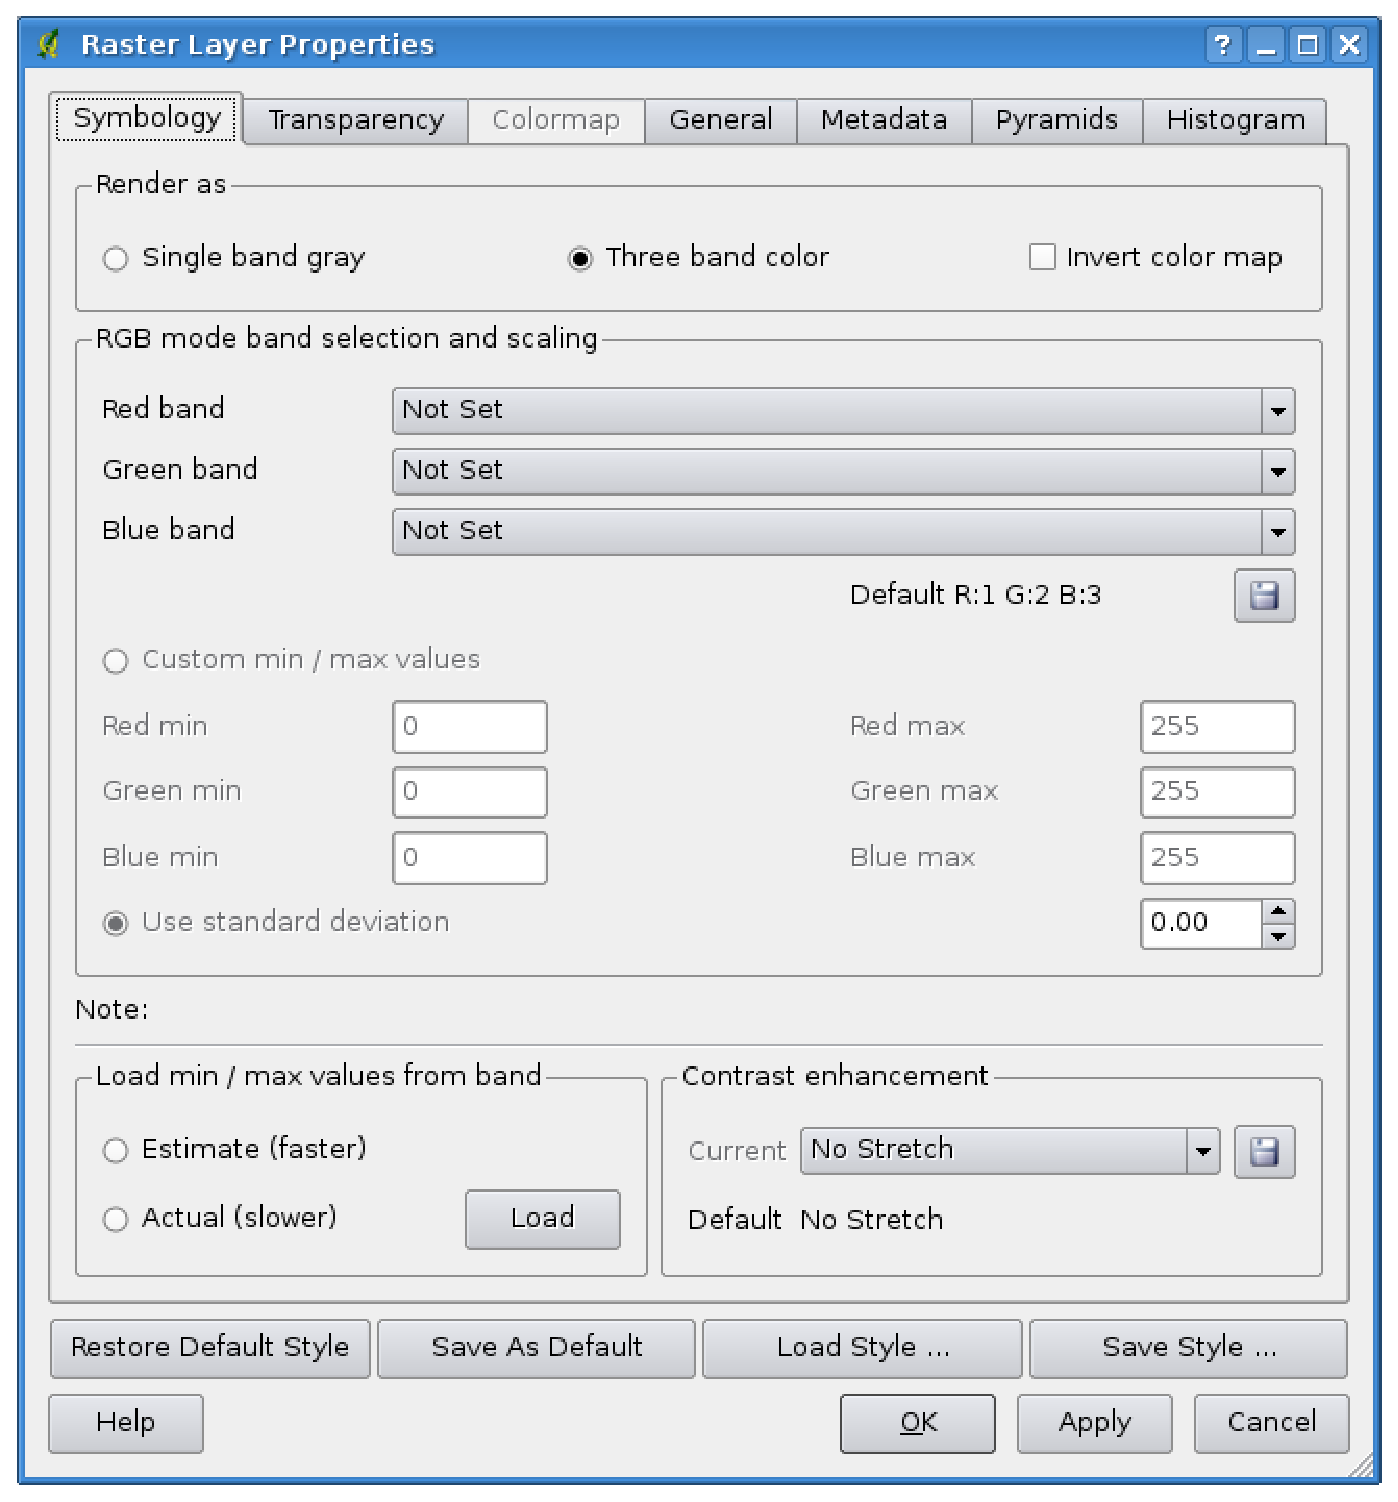
\includegraphics[clip=true, width=14cm]{rasterPropertiesDialog}
\end{center}
\end{figure}

\subsubsection{Onlget s\'emiologie}\label{label_sombology}

% QGIS can render raster layers in two different ways :\index{raster
% layers!supported channels}
QGIS peut afficher des couches raster de deux mani\`eres diff\'erentes
:\index{couches layers!canaux g\'er\'es}

\begin{itemize}
% \item Single band - one band of the image will be rendered as gray or in 
% pseudocolors.
\item Bande simple - une bande de l'image sera affich\'ee en nuance de gris ou en
pseudocouleurs.
% \item Three band color - three bands from the image will be rendered, each 
% band representing the red, green or blue component that will be used to
% create a color image.
\item Trois bandes de couleurs - trois bandes de l'image seront affich\'ees,
chaque bande repr\'esentant le composant rouge, vert ou bleu qui sera utilis\'e
pour cr\'eer une image de couleur.
\end{itemize}

% Within both rendertypes you can invert the color output using the 
% \checkbox{Invert color map} checkbox.
Pour les deux types de rendu vous pouvez inverser la sortie couleur en
utilisant la case \`a cocher \checkbox{Inverser la carte de couleur}

% \minisec{Single Band Rendering}
\minisec{Rendu des bandes simples}

% This selection offers you two possibilites to choose. At first you can
% select which band you like to use for rendering (if the dataset has more than 
% one band).
Ce choix vous permet deux possibilit\'es : vous pouvez d'abord s\'electionner
quelle bande vous voulez utiliser pour le rendu (si le jeu de donn\'ees a plus
d'une bande).

% The second option offers a selection of available colortables for rendering.
La seconde option vous offre une s\'election des tables de couleurs disponibles
pour le rendu.

% The following settings are available through the dropdownbox
% \selectstring{color map}{Grayscale}, where grayscale is the default setting.
Les param\`etres suivants sont disponibles \`a travers la liste d\'eroulante
\selectstring{carte de couleur}{Niveau de gris}, o\`u niveau de gris est le 
param\`etre par d\'efaut.

% Also available are
Sont aussi disponible :
\begin{itemize}
% \item Pseudocolor
\item Pseudo-couleur
% \item Freak Out
\item Pseudo-couleur psych\'ed\'elique
% \item Colormap
\item Couleurs index\'ees
\end{itemize}

% When selecting the entry \selectstring{color map}{Colormap}, the tab
% \tab{Colormap} becomes available. See more on that at chapter
% \ref{label_colormaptab}.
Quand vous s\'electionnez \selectstring{couleurs index\'ees}{Colormap}, l'onglet
\tab{Couleurs index\'ees} est disponible. Plus d'informations dans le chapitre
\ref{label_colormaptab}.

% QGIS can restrict the data displayed to only show cells whose values are
% within a given number of standard deviations of the mean for the
% layer.\index{raster layers!standard deviation} This is useful when you have
% one or two cells with abnormally high values in a raster grid that are having
% a negative impact on the rendering of the raster. This option is only
% available for pseudocolor images.
QGIS peut restreindre les donn\'ees affich\'ees pour afficher seulement les
cellules dont la valeur sont dans un nombre donn\'e de d\'eviations standards de
la moyenne pour la couche.\index{couches raster!d\'eviation standard} Cela est
utile quand vous avez une ou deux cellules avec des valeurs anormalement hautes
dans une grille raster qui ont un impact n\'egatif sur le rendu du raster. Cette
option est seulement disponible pour les images en pseudo-couleur.

% \minisec{Three band color}
\minisec{Couleur \`a trois bandes}

% This selection offers you a wide range of options to modify the appereance
% of your rasterlayer. For example you could switch color-bands from the
% standard RGB-order to something else.
Cette s\'election vous offre un large choix d'options pour modifier l'apparence
de votre couche raster. Par exemple, vous pouvez passer les bandes de couleurs
d'un ordre standard RVB \`a un autre.

% Also scaling of colors are available.
L'\'echantillonage des couleurs est \'egalement disponible.

% \begin{Tip}\caption{\textsc{Viewing a Single Band of a Multiband Raster}}
\begin{Tip}\caption{\textsc{Visualiser une seule bande d'un raster
multibande}
% \qgistip{If you want to view a single band (for example Red) of a multiband
% image, you might think you would set the Green and Blue bands to ``Not
% Set''. But this is not the correct way. To display the Red band, 
% set the image type to grayscale, then select Red as the band to use for Gray.
\qgistip{Si vous d\'esirez visualiser une seule bande (par exemple la bande rouge)
d'une image multibande, vous pouvez penser que vous pourriez d\'efinir les bandes
Vertes et Bleue \`a ``Non d\'efinie''. Mais ce n'est pas la mani\`ere correcte. Pour
afficher la bande Rouge d\'efinissez le type d'image \`a nuance de gris, puis
s\'electionnez Rouge comme bande \`a utiliser pour le Gris.
}
\end{Tip} 

% \subsubsection{Transparency Tab} \label{rastertab:transparency}
\subsubsection{Onglet transparence} \label{rastertab:transparency}

% QGIS has the ability to display each raster layer at varying transparency
% levels.\index{raster layers!transparency} Use the transparency slider to
% indicate to what extent the underlying layers (if any) should be visible
% though the current raster layer. This is very useful, if you like to overlay
% more than one rasterlayer, e.g. a shaded relief-map overlayed by a classified
% rastermap. This will make the look of the map more three dimensional.
QGIS a la possibilit\'e d'afficher chaque raster \`a des niveaux de transparence
diff\'erents.\index{couches raster!transparence} Utiliser la barre coulissante de
transparence pour indiquer \`a quel niveau de transparence les couches sous-jacentes
(s'il y en a) pourront \^etre visible \`a travers cette couche raster. Cela est
tr\`es utile, si vous d\'esirez superposer plus d'une couche raster, par exemple
une carte des reliefs ombr\'es superpos\'e par une carte raster classifi\'ee. Cela
rendra la carte encore plus proche de la 3e dimension.

% Additionally you can enter a rastervalue, which should be treated as
% {\em NODATA}.
De plus, vous pouvez entrer une valeur raster qui pourra \^etre trait\'e comme {\em
NODATA}

% An even more flexible way to customize the transparency can be done in the
% \guiheading{Custom transparency options} section.
% The transparency of every pixel can be set in this tab.
Un moyen encore plus flexible pour personnaliser la transparence est possible
dans la section \guiheading{Options de transparence personnalis\'ee}.
La transparence de chaque pixel peut \^etre d\'efinie dans cet onglet.

% As an example we want to set the water of our example rasterfile
% \filename{landcover.tif} to a transparency of 20\%. The following steps
% are neccessary:
Par exemple, nous voulons d\'efinir l'eau de notre fichier raster d'exemple
\filename{landcover.tif} \`a une transparence de 20 \%. Les \'etapes suivantes sont
n\'ecessaire :
\begin{enumerate}
%  \item  Load the rasterfile \filename{landcover}
\item Chargez le fichier raster \filename{landcover}
%  \item Open the \dialog{properties} dialog by double-clicking on the
%  rasterfile-name in the legend or by right-clicking and choosing
%  \dropmenuopt{Properties} from the popup meun.
 \item Ouvrez la bo\^ite de dialogue \dialog{propri\'et\'ees} en double-cliquant sur
le nom du raster dans la l\'egende ou avec un clic droit et en choisissant
\dropmenuopt{Propri\'et\'ees} du menu contextuel.
%  \item select the \tab{Transparency} tab
 \item S\'electionnez l'onglet \tab{Transparence}.
% \item \label{enum:add} Click the \toolbtntwo{mActionNewAttribute}{Add values
% manually} button. A new row will appear in the pixel-list.
  \item \label{enum:add} Cliquez sur le bouton
\toolbtntwo{mActionNewAttribute}{Ajouter des valeurs manuellement}. Une
nouvelle ligne apparait dans la liste des pixels.
%  \item \label{enum:transp} enter the the raster-value (we use 0 here) and
% adjust the  transparency to 20\%
 \item \label{enum:transp} Entrez la valeur du raster (nous utilisons 0 ici)
et ajustez la transparence \`a 20 \%.
%  \item press the \button{Apply} button and have a look at the map
 \item Pressez le bouton \button{Appliquer} et regardez la carte.
\end{enumerate}

% You can repeat the steps \ref{enum:add} and \ref{enum:transp} to adjust
% more values with custom transparency.
Vous pouvez r\'ep\'eter les \'etapes \ref{enum:add} et \ref{enum:transp} pour ajuster
d'autres valeurs avec une transparence personnalis\'ee. 

% As you can see this is quite easy set custom transparency, but it can be
% quite a lot of work. Therefor you can use the button
% \toolbtntwo{mActionFileSave}{Export to file} to save your transparency-list to
% a file. The button \toolbtntwo{mActionAddRasterLayer}{Import from file} loads
% your transparency-settings and applies them to the current rasterlayer.
Comme vous pouvez le voir il est assez facile de d\'efinir une transparence
personnalis\'ee, mais cela peut prendre un peu de temp. Par cons\'equent vous
pouvez utiliser le bouton \toolbtntwo{mActionFileSave}{Exporter dans un
fichier} pour sauver vos param\`etres  de transparence dans un fichier. Le
bouton \toolbtntwo{mActionAddRasterLayer}{Importer \`a partir d'un fichier} 
charge vos param\`etres de transparence et les applique \`a la couche raster actuel.

% \subsubsection{Colormap} \label{label_colormaptab}
 \subsubsection{Carte de couleur} \label{label_colormaptab}
% FIXME: Write me

% The \tab{Colormap} tab is only available, when you have selected a
% single-band-rendering within the tab \tab{Symbology} (see chapt.
% \ref{label_sombology}).
L'onglet \tab{Colormap} est seulement disponible quand vous avez s\'electionn\'e un
rendu \`a une seule bande dans l'onglet  \tab{S\'emiologie} (voir chapitre
\ref{label_sombology}).

% Three ways of color interpolation are available:
Trois mani\`eres de faire une interpolation de couleur sont disponibles :
\begin{itemize}
% \item Discrete
\item discr\`ete ;
% \item Linear
\item li\'enaire ;
% \item Exact
\item exacte.
\end{itemize}

% The button \button{Add Entry} adds a color to the individual color-table.
% Double-Clicking on the value-column lets you inserting a specific value.
% Double clicking on the color-column opens the dialog \dialog{Select
% color} where you can select a color to apply on that value.
Le bouton \button{Ajouter une entr\'ee} ajoute une couleur \`a la table de couleur
individuelle. Double-cliquez sur la colonne valeur vous permet d'ins\'erer une
valeur sp\'ecifique. Double-cliquez sur la colonne couleur ouvre une bo\^ite de
dialogue \dialog{S\'electionner une couleur}  o\`u vous pouvez s\'electionner une
couleur \`a appliquer sur cette valeur.

% Alternativly you can click on the button \toolbtntwo{mActionNewAttribute}{Load
% colormap from Band} , which tries to load the table from the band (if it has
% any).
Alternativement, vous pouvez cliquer sur le bouton
\toolbtntwo{mActionNewAttribute}{charger une carte de couleur \`a partir de
bande}  qui tente de charger la table \`a partir d'une bande (si celle-ci en a
une).

% The block \guiheading{Generate new color map} allows you to create newly
% categorized colormaps. You only need to select the \selectnumber{number of
% classes}{15} you need and press the button \button{Classify}. Currently
% only one \selectstring{Classification mode}{Equal Interval} is
% supported\index{raster layer!classify}.
Le bloc \guiheading{G\'en\`erer une nouvelle carte de couleurs} vous permet de
cr\'eer de nouvelles cartes de couleurs par cat\'egorie. Vosu avez seulement besoin
de s\'electionner le \selectnumber{nombre de classes}{15} dont vous avez besoin
et d'appuyez sur le bouton \button{Classifier}. Actuellement seule un 
\selectstring{mode de classification}{intervals \'egaux} est g\'er\'e\index{couches
raster!classifier}.

% \subsubsection{General Tab}\label{label_generaltab}
\subsubsection{Onglet g\'en\'eral}\label{label_generaltab}

% The \tab{General} tab displays basic information about the selected raster,
% including the layer source and  display name in the legend (which can be
% modified). This tab also shows a thumbnail of the layer, its legend symbol,
% and the palette.\index{raster layers!properties}
L'onglet \tab{G\'en\'eral} affiche des informations basiques sur le raster
s\'electionn\'e, incluant la source de la couche et le nom affich\'e dans la l\'egende
(qui peut \^etre modifi\'e). Cet onglet montre aussi un aper\c{c}u de la couche, le
symbol de la l\'egende, et la palette.\index{couches raster!propri\'et\'es}

% Additionally scale-dependent visability can be set in this tab. You need to
% check the checkbox and set an appropriate scale where your data will be
% displayed in the map canvas.
De plus la visibilit\'e en fonction de l'\'echelle peut \^etre d\'efinie dans cet
onglet. Vous devez activer la case \`a cocher et d\'efinir une \'echelle appropri\'ee \`a
laquelle vos donn\'ees seront affich\'ees dans la fen\^etre de la carte.

% Also the spatial reference system is printed here as a PROJ.4-string. This can
% be modified by hitting the \button{Change} button.
Le syst\`eme de r\'ef\'erence spatial est \'egalement affich\'e ici comme cha\^ine PROJ.4.
Cela peut \^etre modifi\'e en cliquant sur le bouton \button{Changer}.

% \subsubsection{Metadata Tab}\label{label_metatab}
\subsubsection{Onglet m\'eta-donn\'ees}\label{label_metatab}

% The \tab{Metadata} tab displays a wealth of information about the raster
% layer, including statistics about each band in the current raster layer.
% Statistics are gathered on a 'need to know' basis, so it may well be that a
% given layers statistics have not yet been collected.\index{raster
% layers!metadata}
L'onglet \tab{M\'eta-donn\'ees} affiche toute la richesse d'information sur la
couche raster, dont les statistiques sur chaque bande dans la couche raster
actuelle. Les statistiques sont recueillies sur l'id\'ee de la 'n\'ecessit\'e de
savoir', de sorte qu'il est possible qu'une couche n'ait pas de
statistique collect\'ee.\index{couches raster!m\'eta-donn\'ees} 

% This tab is mainly for information. You cannot change any values printed
% inside this tab. To update the statistics you need to change to tab
% \tab{Histogram} and press the button \button{Refresh} on the bottom right,
% see ch. \ref{label_histogram}.
Cet onglet est principalement pour informations. Vous ne pouvez pas modifier
les valeurs qui y sont affich\'ees. Pour mettre \`a jour les statistiques vous
devez aller dans l'onglet \tab{Histogramme} et pressez le bouton
\button{Rafraichir} en bas \`a droite, voir chapitre \ref{label_histogram}.

% \subsubsection{Pyramids Tab}\label{raster_pyramids}
\subsubsection{Onglet pyramides}\label{raster_pyramids}

% Large resolution raster layers can slow navigation in QGIS. By creating lower
% resolution copies of the data (pyramids), performance can be considerably
% improved as QGIS selects the most suitable resolution to use depending on the
% level of zoom.
Les couches raster \`a haute r\'esolution peuvent ralentir la navigation dans QGIS.
En cr\'eant des copies de plus basse r\'esolution des donn\'ees (pyramides), les
performances peuvent \^etre consid\'erablement am\'elior\'ees puisque QGIS s\'electionne
la r\'esolution la plus pertinente \`a utiliser en fonction du niveau de zoom.

% \index{raster layers!pyramids}
\index{couches raster!pyramides}
% \index{raster layers!resolution pyramids}
\index{couches raster!r\'esolution des pyramides}

% You must have write access in the directory where the original data is stored
% to build pyramids. \\
Vous devez avoir acc\`es en \'ecriture dans le r\'epertoire o\`u les donn\'ees
originelles sont stock\'ees pour construire les pyramides. \\
% Several resampling methods can be used to calculate the pyramides:
Plusieurs m\'ethodes de re\'echantillonage peuvent \^etre utilis\'ees pour calculer les
pyramides :
\begin{itemize}
% \item Average
\item moyen
% \item Nearest Neighbour
\item plus proche voisin ;
\end{itemize}

% When checking the checkbox \checkbox{Build pyramids internally if
% possible} QGIS tries to build pyramids internally.
Quand la case \checkbox{construire les pyramides en interne si possible} est
coch\'ee, QGIS tente de construire les pyramides en interne.

% Please note that building pyramids may alter the original data file and once
% created they cannot be removed. If you wish to preserve a 'non-pyramided'
% version of your raster, make a backup copy prior to building pyramids.
S'il vous plait notez que construire des pyramides peut alt\'erer les fichiers
donn\'ees originaux et une fois cr\'e\'e ils ne peuvent plus \^etre supprim\'e. Si vous
d\'esirez pr\'eserver une version 'sans pyramide' de vos raster, r\'ealisez une copie
de sauvegarde avant de les construire.

% \subsubsection{Histogram Tab}\label{label_histogram}
\subsubsection{Onglet histograme}\label{label_histogram}

% The \tab{Histogram} tab allows you to view the distribution\index{raster
% layers!histogram} of the bands or colors in your raster. You must first
% generate the raster statistics by clicking the \button{Refresh} button. You
% can choose which bands to display by selecting them in the list box at the
% bottom left of the tab. Two different chart types are allowed: 
L'onglet \tab{Histogramme}  vous permet de visualiser la distribution
\index{couches raster!histogramme} des bandes ou des couleurs dans votre
raster. Vous devez d'abord g\'en\'erer les statistiques du raster en cliquant le
bouton \button{Rafraichir}. Vous pouvez choisir quelles bandes \`a afficher en
les s\'electionnant dans la liste d\'eroulante en bas \`a gauche de l'onglet. Deux
types de graphiques diff\'erents sont permis :

\begin{itemize}
% \item Bar chart
\item graphique en barre ;
% \item Line graph
\item graphique lin\'eaire ;
\end{itemize}

% You can define the number of chart columns to use and decide wether you want 
% to \checkbox{Allow approximation} or display \checkbox{out of range} values 
% Once you view the histogram, you'll notice that the band statistics have been
% populated on the \tab{metadata} tab.\index{raster layers!metadata)}
Vous pouvez d\'efinir le nombre de colonnes du graphique \`a utiliser et d\'ecider si
vous voulez \checkbox{Permettre l'approximation} ou afficher les valeurs
\checkbox{En dehors du domaine}. Une fois que vous avez vu l'histogramme, vous
remarquerez que les statistiques des bandes ont \'et\'e remplies dans l'onglet
\tab{m\'eta-donn\'ees}.\index{couches raster!m\'eta-donn\'ees}

% \begin{Tip}\caption{\textsc{Gathering Raster Statistics}}
\begin{Tip}\caption{\textsc{Regroupement des statistiques raster}}
% \qgistip{To gather statistics for a layer, select pseudocolor rendering and
% click the \button{Apply} button. Gathering statistics for a layer can be time
% consuming. Please be patient while QGIS examines your
% data!\index{raster layers!statistics}
\qgistip{Rassembler des statistiques pour une couche, s\'electionnez un rendu en
pseudo-couleur et cliquez sur le bouton \button{Appliquer}. Regrouper des
statistiques pour une couche peut prendre du temp. Soyez patient pendant que
QGIS examine  vos donn\'ees !\index{couches raster!statistiques}
}
\end{Tip}

% vim:autoindent:set textwidth=78:

\section{Arbeiten mit Projektionen}\label{label_projections}
\index{Koordinatenbezugssystem}\index{Projektion}

% when the revision of a section has been finalized, 
% comment out the following line:
%\updatedisclaimer

QGIS erm�glicht es, globale und projektbezogene KBS (Koordinatenbezugssysteme)
f�r Layer ohne vordefinierte KBS zu definieren. Es k�nnen benutzerdefinierte
Koordinatenbezugssysteme erstellt werden und f�r Vektorlayer wird On-The-Fly
(OTF) Projektion unterst�tzt, um Layer gemeinsam und lagegenau darzustellen,
obwohl sie unterschiedliche KBS besitzen. 

\subsection{�berblick zur Projektionsunterst�tzung}\label{label_projoverview}

QGIS unterst�tzt etwa 2700 bekannte Koordinatenbezugssysteme (KBS). Diese
sind in einer SQlite-Datenbank abgelegt, die mit QGIS installiert wird.
Normalerweise muss diese Datenbank nicht editiert werden, und es kann
Probleme verursachen, wenn Sie es dennoch versuchen. Selbst definierte KBS
sind in einer Benutzerdatenbank abgelegt. Informationen zum Anlegen einer
Benutzerdatenbank finden Sie im Abschnitt \ref{sec:customprojections}.

Die Koordinatenbezugssysteme in QGIS basieren auf EPSG Codes\index{EPSG} und
sind weitestgehend der spatial\_references Tabelle von PostGIS\index{PostGIS}
Version 1.x entnommen. Wichtig ist, dass die IDs, welche von QGIS benutzt
werden, nicht den IDs der spatial\_references Tabelle oder den EPSG Codes
entsprechen. Die EPSG und PostGIS IDs sind in der SQlite-Datenbank abgelegt
und werden benutzt, um KBS in QGIS zu spezifizieren.

Um OTF Projektion zu verwenden, m�ssen die Daten Informationen �ber ihr
Koordinatenbezugssystem enthalten. Bei PostGIS-Layern benutzt QGIS die spatial
reference ID, die bei der Erstellung des Layers festgelegt wurde. Bei Daten,
die von der OGR-Bibliothek unterst�tzt werden, bezieht sich QGIS auf das
Vorhandensein eines KBS bei den Daten. Bei Shapes bedeutet dies, dass eine
Datei mit der Endung .prj vorhanden sein muss, in der das KBS im Well
Known Text (WKT)\index{WKT} Format angegeben ist. F�r ein Shape mit dem Namen
\filename{lakes.shp} g�be es also eine entsprechende Projektionsdatei
\filename{lakes.prj}. 

\subsection{Ein Koordinatenbezugssystem festlegen}
\index{Koordinatenbezugssystem!festlegen}
\label{sec:projection-specifying}

QGIS setzt das Koordinatenbezugssystem beim Start nicht mehr automatisch auf
das KBS des zuerst geladenen Layers. Wenn Sie QGIS mit einem Layer starten,
der keine KBS-Informationen bereitstellt, m�ssen Sie f�r diesen Layer ein
KBS festlegen. Dies kann global oder projektbezogen im Reiter \tab{KBS} im
Men� \mainmenuopt{Einstellungen} > \dropmenuopttwo{mActionOptions}{Optionen}
geschehen (Siehe Abbildung~\ref{fig:crsdialog}) 

\begin{itemize}
\item \checkbox{KBS abfragen} 
\item \checkbox{Projektweite KBS-Voreinstellung}
\item \checkbox{Untenstehende globale Voreinstellung wird genutzt}
\end{itemize}

Das globale standard Koordinatenbezugssystem \usertext{proj=longlat
+ellps=WGS84 +datum=WGS84 +no\_defs} ist vordefiniert in QGIS, kann aber
nat�rlich ge�ndert werden und wird dann f�r folgende Sitzungen gespeichert. 

\begin{figure}[ht]
   \begin{center}
   \caption{KBS Reiter im Dialog Optionen \nixcaption}\label{fig:crsdialog}\smallskip
   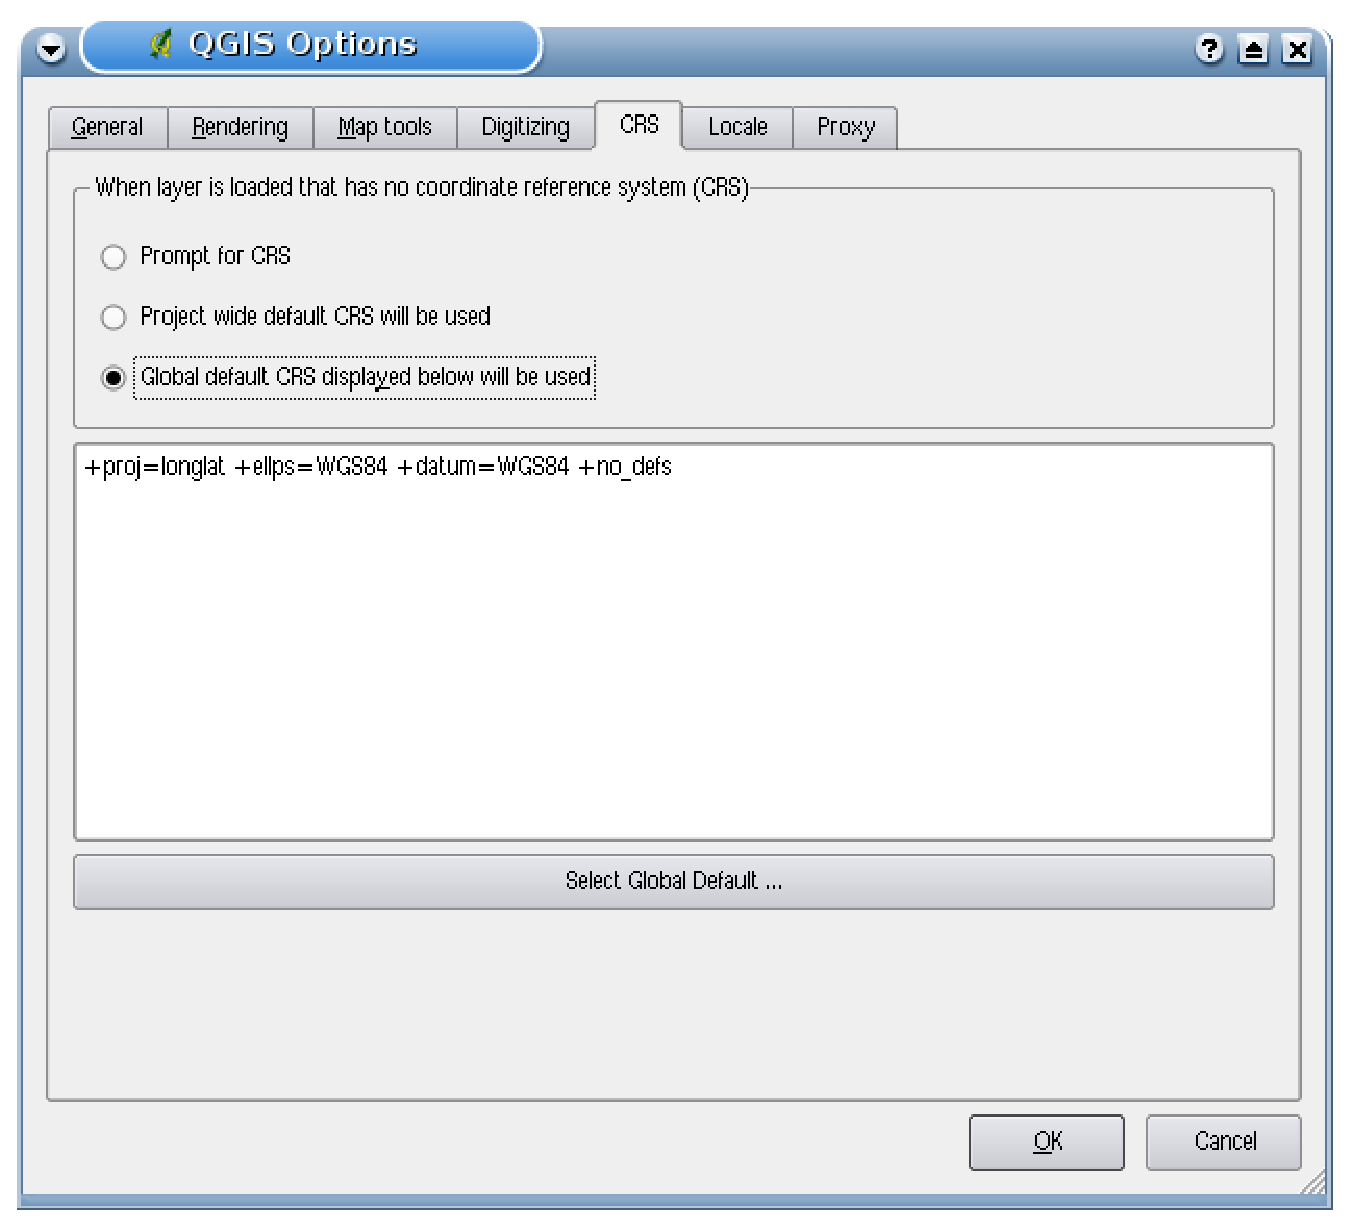
\includegraphics[clip=true, width=11cm]{crsdialog}
\end{center}
\end{figure}

Wenn Sie ein Koordinatenbezugssystem f�r einen bestimmten Layer festlegen
m�chten, k�nnen Sie das im Reiter \tab{Allgemein} der Dialoge f�r 
Rasterlayereigenschaften (\ref{label_generaltab}) und
Vektorlayereigenschaften (\ref{vectorgeneraltab}) machen. Falls der geladene
Layer bereits Informationen zu seinem Koordinatenbezugssystem enth�lt,
werden diese angezeigt (siehe Abbildung~\ref{fig:vector_symbology}).

\subsection{On-The-Fly (OTF) Projektion}\label{label_projstart}

In QGIS ist die Unterst�tzung f�r On-The-Fly (OTF) Projektion nicht als
Standard aktiviert. Um diese auszuw�hlen, �ffnen Sie den Dialog
\dropmenuopttwo{mActionOptions}{Projekteinstellungen}, wechseln in den Reiter
\tab{Benutzerkoordinatenreferenzsystem} und klicken dort auf das
Kontrollk�stchen \checkbox{On-The-Fly-KBS-Transformation aktivieren}. 

Um den Dialog \tab{Benutzerkoordinatenreferenzsystem} zu �ffnen, k�nnen Sie
auch auf das Icon \toolbtntwo{mIconProjectionEnabled}{KBS-Status} in der
unteren rechten Ecke der Statusleiste dr�cken.

Wenn Sie bereits einen Layer geladen haben und nun die Unterst�tzung f�r
On-The-Fly (OTF) Projektion aktivieren wollen ist der beste Weg folgender.
�ffnen Sie den Reiter \tab{Benutzerkoordinatenreferenzsystem} im Men�
\dropmenuopttwo{mActionOptions}{Projekteinstellungen}, w�hlen Sie das
passende KBS f�r den Layer aus und aktivieren Sie dann das
Kontrollk�stchen \checkbox{On-The-Fly-KBS-Transformation aktivieren}. Alle
daraufhin geladenen Vektorlayer werden werden dann On-The-Fly auf das
ausgew�hlte KBS projiziert. 

Der Reiter \tab{Benutzerkoordinatenreferenzsystem} enth�lt vier wichtige
Optionen (siehe Abbildung~\ref{fig:projections}). Diese werden im Folgenden
beschrieben.

\begin{figure}[ht]
   \begin{center}
   \caption{Dialog Projekteinstellungen \nixcaption}\label{fig:projections}\smallskip
   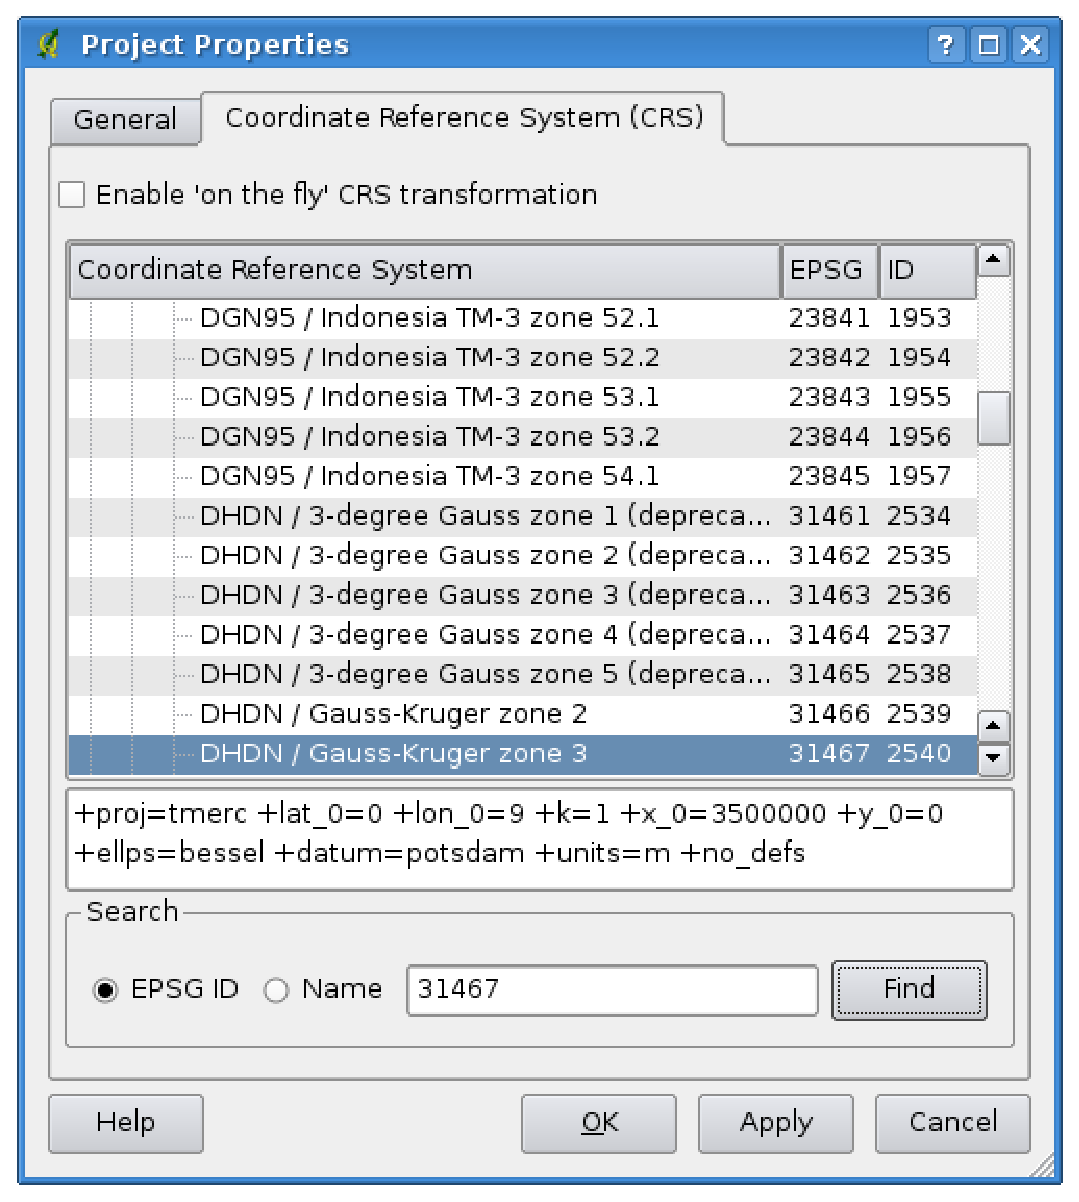
\includegraphics[clip=true, width=11cm]{projectionDialog}
\end{center}  
\end{figure}

\begin{enumerate}
\item \textbf{On-The-Fly-KBS-Transformation
aktivieren}\index{Koordinatenbezugssystem!OTF!aktivieren} 
- �ber diese Checkbox wird die OTF Projektion aktiviert oder deaktiviert.
  Wenn sie deaktiviert ist, wird jeder Layer entsprechend seines KBS
  dargestellt. Wenn es aktiviert ist, wird jeder Layer beim Laden in die
definierte Koordinatenbezugssystem 'on-the-fly' umgewandelt dargestellt.
\item \textbf{Koordinatensystem} - dies ist eine Liste mit allen
Koordinatenbezugssystemen, die von QGIS unterst�tzt werden. Um ein
KBS zu benutzen, w�hlt man es aus der Liste aus. Die bis dahin aktive
Projektion ist vorgegeben als WGS 84.
\item \textbf{Proj4 Text} - dies ist ein Ausdruck, der von der PROJ-Bibliothek
genutzt wird. Es dient nur zur Information und kann nicht ver�ndert werden.
\item \textbf{Suchen} - wenn Sie den EPSG Code oder den Namen f�r ein KBS
kennen, k�nnen Sie diese benutzen, um ihr Koordinatenbezugssystem zu finden.
Geben Sie eine ID  der Namen ein und klicken Sie auf \button{Finden}.
\end{enumerate}

\begin{Tip}
\caption{\textsc{Dialog Projekteigenschaften}}
\qgistip{Wenn Sie den Dialog \dialog{Projekteigenschaften} �ber die
Men�leiste �ffnen, m�ssen Sie erst auf den Reiter
\tab{Benutzerkoordinatenreferenzsystem} dr�cken. �ber das
\toolbtntwo{mIconProjectionEnabled}{KBS-Status} Icon in der Statusleiste
unten rechts wird der Reiter \tab{Benutzerkoordinatenreferenzsystem} direkt
in den Vordergrund ger�ckt.
}
\end{Tip}

\subsection{Ein Koordinatenbezugssystem selbst definieren}\label{sec:customprojections}
\index{Koordinatenbezugssystem!anpassen}

Wenn QGIS nicht das KBS bereith�lt, welches Sie brauchen, k�nnen Sie ein
eigenes KBS erstellen. Dazu w�hlen Sie in der Men�leiste
\mainmenuopt{Einstellungen} >
\dropmenuopttwo{mIconNew}{Benutzerkoordinatenbezugssystem}. Das eigene KBS
wird in einer Benutzerdatenbank erstellt. Diese enth�lt Ihre r�umlichen
Lesezeichen und die selbst erstellten Projektionen.

\begin{figure}[ht]
   \begin{center}
   \caption{Definition eines eigenen Koordinatenbezugssystems \nixcaption}\label{fig:customprojections}\smallskip
   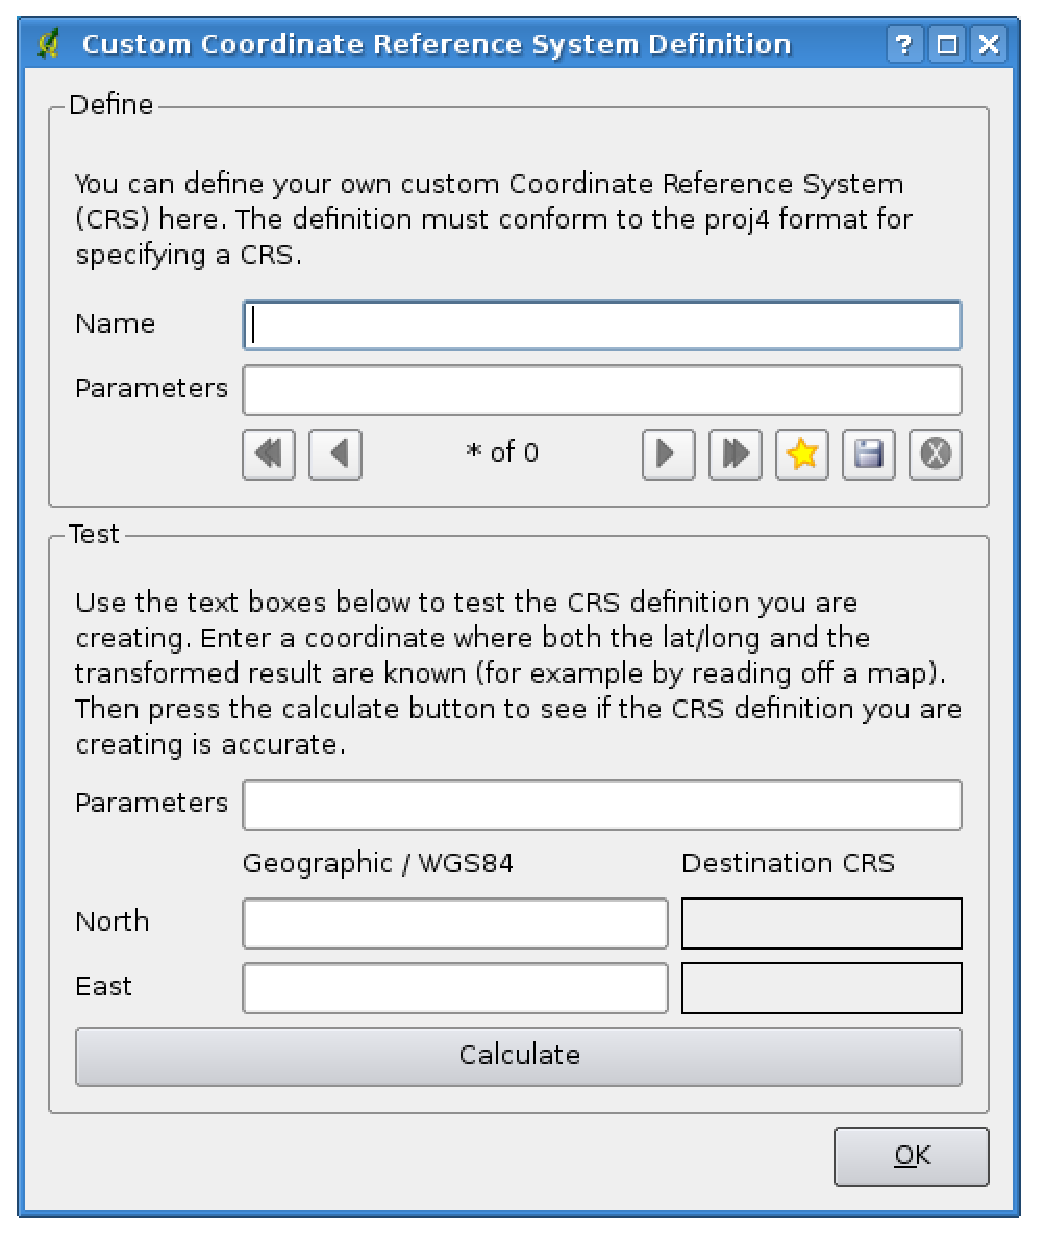
\includegraphics[clip=true, width=11cm]{customProjectionDialog}
\end{center}  
\end{figure}

In QGIS bedarf es einem grundlegenden Verst�ndnis im Umgang mit der
PROJ4-Bibliothek. Zu Beginn sollten Sie einen Blick in das Benutzerhandbuch
von PROJ werfen. Cartographic Projection Procedures for the UNIX Environment
- A User's Manual by Gerald I. Evenden, U.S. Geological Survey Open-File Report
90-284, 1990 (zu finden unter \url{ftp://ftp.remotesensing.org/proj/OF90-284.pdf}).
Dieses Handbuch beschreibt die Anwendung von \usertext{proj.4}. Die dort
beschriebenen kartographischen Parameter sind identisch mit denen, die in QGIS
verwendet werden.

Der Dialog \dialog{Definition eines Benutzerkoordinatenbezugssystem} braucht
nur zwei Eintr�ge, um eine eigene Projektion zu definieren:

\begin{enumerate}
\item Einen Namen
\item kartographische Parameter 
\end{enumerate}

Um ein neues KBS zu erstellen, klicken Sie auf den Knopf
\toolbtntwo{mIconNew}{Neu}, geben Sie einen beschreibenden Namen ein
und die kartographischen Parameter. Abbildung \ref{fig:customprojections}
zeigt den Dialog mit einer Beispielprojektion. Danach speichern Sie das neue
KBS mit dem Knopf \toolbtntwo{mActionFileSave}{Speichern} ab. 

Denken Sie daran, dass die kartographischen Parameter mit einem
\usertext{+proj=}-Block beginnen m�ssen, um den Beginn eines neuen KBS
anzuzeigen. 

Sie k�nnen das neue KBS testen, um zu sehen, ob bei einer Konvertierung
von bekannten WGS84 Lat-Lon Koordinaten in ihre Projektion ein sinnvolles
Ergebnis herauskommt. Dazu kopieren Sie ihre kartographischen Parameter in
das Fenster \guilabel{Parameter}, geben ein paar bekannte WGS84 Lat-Lon
Koordinaten an und klicken dann auf den Knopf \button{Berechnen}. Vergleichen
Sie die Ergebnisse mit den Werten im Kartenfenster.



\section{Integración de GRASS}\label{sec:grass}\index{GRASS}

El complemento de GRASS~\cite{GRASSweb} proporciona acceso a GRASS desde dentro de QGIS. Esto incluye la capacidad de ver, editar y crear datos, así como realizar análisis usando los módulos de geoprocesamiento de GRASS.

En este capítulo presentaremos el complemento y alguna de las formas que se pueden usar para trabajar con datos de GRASS. El complemento de GRASS proporciona las siguientes funciones:
 
\begin{itemize}
\item \includegraphics[width=0.7cm]{add_grass_vector} Añadir capas vectoriales de GRASS.
\item \includegraphics[width=0.7cm]{add_grass_raster} Añadir capas ráster de GRASS.
\item 
\includegraphics[width=0.7cm]{grass_tools} Caja de herramientas de GRASS.
\item \includegraphics[width=0.7cm]{grass_region_edit} Cambiar la región de GRASS.
\item 
\includegraphics[width=0.7cm]{grass_edit} Digitalización de capas vectoriales.
\item 
\includegraphics[width=0.7cm]{grass_open_mapset} Abrir directorios de mapas existentes.
\item 
\includegraphics[width=0.7cm]{grass_new_mapset} Crear nuevos directorios de mapas.
\item 
\includegraphics[width=0.7cm]{grass_new_vector_layer} Crear nuevas capas vectoriales de GRASS.
\item 
\includegraphics[width=0.7cm]{grass_close_mapset} Cerrar directorios de mapas de GRASS.
\end{itemize}

\subsection{Iniciar QGIS con GRASS}\label{sec:starting_grass}
\index{GRASS!starting QGIS}

Para usar las funciones de GRASS desde dentro de QGIS, debe cargar el complemento de GRASS con el administrador de complementos (vea la Sección \ref{sec:managing_plugins}) como todos los complementos de QGIS. Después de cargarlo, aparecerá una nueva barra de herramientas en la interfaz de usuario.\footnote{El complemento de GRASS es único en cuanto que crea su propia barra de herramientas}

Después de cargar el complemento, inmediatamente puede cargar un conjunto de datos vectoriales y ráster de GRASS existente (vea la Sección \ref{sec:load_grassdata}) o puede crear una nueva localización de GRASS con QGIS (vea la Sección \ref{sec:create_loc}).

\subsection{Cargar datos de GRASS}\label{sec:load_grassdata}\index{GRASS!loading data}

Con el complemento de GRASS, puede cargar capas vectoriales o ráster usando los botones adecuados de la barra de herramientas. Como ejemplo usaremos la localización spearfish de muestra en proyección UTM (vea la Sección \ref{label_sampledata}).

\begin{enumerate}
  \item Descargue el archivo spearfish\_grass60data-0.3.zip.
  \item Cree una carpeta nueva \textsl{grassdata} y descomprima en ella el archivo spearfish\_grass60data-0.3.zip.
  \item Inicie QGIS.
  \item En la barra de herramientas de GRASS, pulse el icono \textsl{Abrir directorio de mapas} para iniciar el asistente \textsl{Seleccionar directorio de mapas de GRASS}.
  \item Para la \textsl{Base de datos} explore e introduzca la ruta a la carpeta recién creada \textsl{grassdata}.
  \item Ahora debería poder seleccionar la localización \textsl{spearfish60} y los directorios de mapas \textsl{PERMANENT} o \textsl{user1}. 
  \item Pulse \textsl{Aceptar}. Note como algunas de las herramientas de la barra de herramientas de GRASS que estaban desactivadas ahora están activadas.
  \item Pulse en \textsl{Añadir capa ráster de GRASS}, seleccione el \textsl{Nombre del mapa} geology y pulse \textsl{Aceptar}. El mapa geology se visualizará. 
  \item Pulse en \textsl{Añadir capa vectorial de GRASS}, seleccione el \textsl{Nombre del mapa} roads (carreteras) y pulse \textsl{Aceptar}. Ahora el mapa roads se superpondrá encima de la geología.  
\end{enumerate}

Como puede ver, es muy sencillo cargar capas ráster y vectoriales de GRASS en QGIS. Vea las siguientes secciones para editar datos de GRASS y crear nuevas localizaciones.

\begin{Tip}\caption{\textsc{Cargar datos de GRASS}}
\qgistip{Si tiene problemas para cargar datos o QGIS termina de forma anormal, asegúrese de que ha cargado el complemento de GRASS correctamente como se describe en la Sección \ref{sec:starting_grass}.
}
\end{Tip} 

\subsection{Crear una localización}\label{sec:create_loc}

GRASS guarda los datos en una ``localización'' que representa un área específica con un sistema de coordenadas específico. Para usar datos de GRASS, debemos importarlos a una \textsl{localización}.\footnote{Esto no es estrictamente cierto, se pueden ver conjuntos de datos externos sin importarlos}

\begin{figure}[ht]
   \begin{center}
   \caption{Crear una localización de GRASS en QGIS}\label{fig:grass_location}\smallskip
   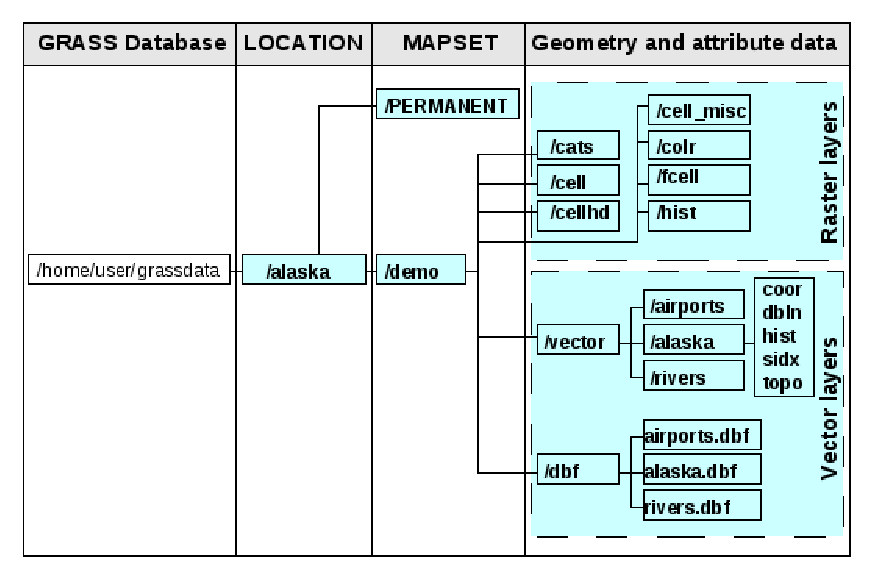
\includegraphics[clip=true, width=8cm]{grass_location}
\end{center}  
\end{figure}

Aquí tiene un ejemplo de cómo crear una localización de GRASS en la proyección Albers Equal Area con unidades en metros para los datos de ejemplo de QGIS (vea la Sección \ref{label_sampledata}). 

\begin{enumerate}
  \item Inicie QGIS.
  \item Asegúrese de que el complemento de GRASS está cargado.
  \item Cargue el archivo shape \textsl{alaska.shp} (vea la Sección \ref{sec:load_shapefile}).
  \item En la barra de herramientas de GRASS, pulse en la herramienta \textsl{Nuevo directorio de mapas} para llamar al asistente directorio de mapas.
  \item Cada localización se guarda en un directorio. Seleccione un directorio de datos existente o cree uno nuevo para guardar la localización.
  \item Pulse \textsl{Siguiente}.
  \item Podemos usar el asistente para crear un nuevo directorio de mapas dentro de una localización existente o crear una nueva localización todo junto. Marque el botón circular ``Crear nueva localización''.
  \item Introduzca un nombre para la localización (usaremos Alaska).
  \item Pulse \textsl{Siguiente}.
  \item Defina la proyección pulsando el botón circular ``Proyección'' para activar la lista de proyecciones.
  \item Estamos usando la proyección Albers Equal Area Alaska (metros). Como sabemos que su SRID de PostGIS es 5000, lo introducimos en la casilla de búsqueda. (Si quiere repetir este proceso para otra capa y no recuerda el SRID de PostGIS, pulse en el icono del proyector en la esquina inferior derecha de la barra de estado (vea la Sección \ref{label_projstart}).)
  \item Pulse \textsl{Encontrar} para seleccionar la proyección.
  \item Pulse \textsl{Siguiente}.
  \item Para definir la región predeterminada, tenemos que introducir los límites en dirección Norte, Sur, Este y Oeste. Aquí simplemente pulsaremos el botón \textsl{Establecer la extensión actual de QGIS}.
  \item Pulse \textsl{Siguiente}. 
  \item Tenemos que definir un directorio de mapas dentro de nuestra nueva localización. Póngale el nombre que prefiera (su nombre de usuario es una buena opción).
  \item Compruebe el resumen para asegurarse que es correcto.
  \item Pulse \textsl{Terminar} 
  \item El directorio de mapas y la localización son creados y se abren como el conjunto de trabajo actual.
  \item Vea como algunas de las herramientas de la barra de herramientas de GRASS que estaban desactivadas ahora están activadas para su uso.
\end{enumerate}

Si le parecieron muchos pasos, ésto no es tan malo y sí una forma muy rápida de crear una localización. Nuestra localización ahora está lista para usar. Para ver la región predeterminada, aleje el zum. Pulsando la herramienta \textsl{Mostrar región actual de Grass} se activa/desactiva la visualización de la región.

\subsection{Modelo de datos vectoriales}\label{label_vectmodel}\index{GRASS!vector data model}

Es importante entender el modelo de datos vectoriales de GRASS antes de digitalizar.\index{GRASS!digitizing} En general, GRASS usa un modelo vectorial topológico.\index{GRASS!topology} Esto significa que las áreas no se representan como polígonos cerrados, sino por uno o más contornos. Esto significa que las áreas no se representan como polígonos cerrados, sino por uno o más contornos. Los contornos deben estar conectados sin saltos. Un área es identificada (etiquetada) por los centroides del área.

Además de contornos y centroides, un mapa vectorial puede contener puntos y líneas. Todos estos elementos geométricos pueden mezclarse en un vectorial y se representarán en las llamadas «capas» en QGIS.

Es posible guardar más «capas» en un conjunto de datos vectorial. Por ejemplo, se pueden guardar campos, bosques y lagos en un vectorial. Los bosques y lagos adyacentes pueden compartir el mismo contorno, pero tiene tablas de atributos separadas. También es posible adjuntar atributos a los contornos. Por ejemplo, el contorno entre lago y bosque es una carretera, por lo que puede tener una tabla de atributos diferente.

La «capa» de los objetos espaciales se define por la «capa» dentro de GRASS. «Capa» es un número que define si hay más de una capa dentro del conjunto de datos, por ejemplo, si la geometría es bosque o lago. De momento, puede ser sólo un número, en el futuro GRASS también soportará nombre como campos en la interfaz de usuario.

Los atributos se pueden guardar en bases de datos externas, por ejemplo DBF, PostgreSQL, MySQL, SQLite3, etc.\index{GRASS!attribute storage}

Los atributos en las tablas de las bases de datos se enlazan a los elementos geométricos usando la «categoría».\index{GRASS!attribute linkage} La «categoría» (clave, ID) es un entero adjunto a los primitivos de la geometría y se usa como el enlace a una columna de la tabla de la base de datos.

\begin{Tip}\caption{\textsc{Aprender el modelo vectorial de GRASS}}
\qgistip{La mejor forma de aprender el modelo vectorial de GRASS y sus capacidades es descargar uno de los muchos manuales de GRASS, donde se describe el modelo vectorial con más detalle. Vea \url{http://grass.osgeo.org/gdp/manuals.php} para más información, libros y manuales en varios idiomas.
}
\end{Tip} 

\subsection{Herramientas de digitalización y edición}\index{GRASS!digitizing tools}
\label{grass_digitising}


\includegraphics[width=0.7cm]{grass_edit} Las herramientas de digitalización para las capas vectoriales de GRASS son accesibles usando la herramienta \textsl{Editar capa vectorial de GRASS} de la barra de herramientas. Asegúrese de que ha cargado un vectorial de GRASS y que éste es la capa seleccionada en la leyenda antes de pulsar la herramienta de edición. Si quiere crear un nuevo vectorial de GRASS, necesita usar la entrada de menú Complementos->GRASS->Crear nuevo vectorial de GRASS o el icono de la barra de herramientas de Grass.

La figura \ref{fig:grass_edit} muestra el diálogo de edición de GRASS que se muestra cuando se pulsa la herramienta de edición.

\begin{figure}[h]
   \begin{center}
   \caption{Diálogo de edición de GRASS}\label{fig:grass_edit}\smallskip
   \includegraphics[clip=true, width=13cm]{grassedit}
\end{center}  
\end{figure}

Las herramientas y la configuración se tratan en las siguientes secciones.

\subsubsection{Barra de herramientas}\label{label_grasstoolbar}

La tabla \ref{tab:grass_tools} lista las herramientas de digitalización proporcionadas por el complemento de GRASS. Éstas corresponden a los botones de herramientas en la barra de herramientas de la parte superior del diálogo.

\begin{table}[h]\index{GRASS!digitizing tools}
\centering
\caption{Herramientas de digitalización de GRASS}\label{tab:grass_tools}\medskip
 \begin{tabular}{|l|l|p{5in}|}
 \hline \textbf{Icono} & \textbf{Herramienta} & \textbf{Propósito} \\
\hline 
\includegraphics[width=0.7cm]{grass_new_point} & Nuevo punto & Digitalizar un punto nuevo \\
\hline 
\includegraphics[width=0.7cm]{grass_new_line} & Nueva línea &  Digitalizar una línea nueva (finaliza al seleccionar una herramienta nueva) \\
\hline 
\includegraphics[width=0.7cm]{grass_new_boundary} & Nuevo contorno & Digitalizar un contorno nuevo (finaliza al seleccionar una herramienta nueva)\\
\hline 
\includegraphics[width=0.7cm]{grass_new_centroid} & Nuevo centroide & Digitalizar un centroide nuevo (etiquetar un área existente)\\
\hline \includegraphics[width=0.7cm]{grass_move_vertex} & Mover vértice & Seleccionar un vértice de una línea o contorno existente e identificar una nueva posición\\
\hline 
\includegraphics[width=0.7cm]{grass_add_vertex} & Añadir vértice & Añadir un vértice nuevo a una línea existente\\
\hline 
\includegraphics[width=0.7cm]{grass_delete_vertex} & Borrar vértice & Borrar un vértice de una línea existente (confirmar el vértice seleccionado con otra pulsación)\\
\hline \includegraphics[width=0.7cm]{grass_move_line} & Mover elemento & Seleccionar un elemento existente y pulsar en la nueva posición\\
\hline 
\includegraphics[width=0.7cm]{grass_split_line} & Dividir línea & Dividir una línea existente en dos partes\\
\hline \includegraphics[width=0.7cm]{grass_delete_line} & Borrar elemento & Borrar un elemento existente (confirmar el elemento seleccionado con otra pulsación)\\
\hline 
\includegraphics[width=0.7cm]{grass_edit_attributes} & Editar atributos & Editar los atributos de un elemento existente (tenga en cuenta que un elemento puede representar a más objetos espaciales, vea arriba)\\
\hline \includegraphics[width=0.7cm]{grass_close_edit} & Cerrar & Cerrar la sesión de digitalización (reconstruye la topología a continuación)\\
\hline
\end{tabular}
\end{table}

\subsubsection{Pestaña Categoría}\index{GRASS!category settings}

Esta pestaña le permite establecer la forma en que se asignará la categoría a cada nuevo objeto espacial y/o asignar una categoría a un objeto espacial.

\begin{itemize}
\item Modo: qué categoría se debería adjuntar a la geometría.
\begin{itemize}
\item La siguiente sin usar: la siguiente categoría que aún no está usada en el archivo vectorial.
\item Entrada manual: definir la categoría en el campo de entrada «Categoría».
\item Ninguna categoría: digitalizar la geometría sin introducir ninguna categoría.
\end{itemize}
\item Categoría: un número (ID) que se adjunta al objeto espacial digitalizado.
\item Capa: identificación del objeto espacial (tabla de atributos).
\end{itemize}

\begin{Tip}\caption{\textsc{Crear «capas» adicionales con QGIS}}
\qgistip{Si quiere añadir más capas a su conjunto de datos, simplemente añada un nuevo número en la casilla «Capa» y pulse Intro. En la pestaña Tabla puede crear una nueva tabla conectada a su nueva capa.
}
\end{Tip}

\subsubsection{Pestaña configuración}\label{label_settingtab}\index{GRASS!snapping tolerance}

Esta pestaña le permite establecer el autoensamblado en píxeles de la pantalla. Esto es el umbral en píxeles en el que los nuevos puntos o finales de líneas son ensamblados de forma automática a nodos existentes. Esto ayuda a evitar saltos o balanceos entre contornos. El valor predeterminado es 10 píxeles.

\subsubsection{Pestaña simbología}\index{GRASS!symbology settings}

Esta pestaña le permite ver y establecer la simbología y la configuración del color para varios tipos de geometría y su estado topológico (ej.: contorno cerrado / abierto).

\subsubsection{Pestaña tabla} \index{GRASS!table editing}
Esta pestaña proporciona información sobre la tabla de la base de datos de una «capa» dada. Aquí puede añadir, modificar o crear nuevas tablas de base de datos para la capa actual.

\begin{Tip}\caption{\textsc{Permisos de edición de GRASS}}\index{GRASS!edit
permissions}
\qgistip{Tiene que ser el propietario del directorio de mapas de GRASS que quiera editar. Es imposible editar vectoriales en directorios de mapas que no sean suyos, incluso si tiene permiso de escritura.
}
\end{Tip} 

\subsection{Herramienta Región}\index{GRASS!region}

\includegraphics[width=0.7cm]{grass_region_edit} La región actual (ventana) en GRASS es muy importante para todos los módulos ráster. Todos los ráster de nueva creación tienen la extensión y resolución de la región actual, no importa cuál sea su región original. La región se guarda en el archivo \$LOCATION/\$MAPSET/WIND, y define el Norte, Sur, Este, Oeste, número de columnas y filas y la resolución espacial horizontal y vertical.

Es posible encender/apagar la región de GRASS en la vista del mapa de QGIS usando el botón \textsl{Mostrar región actual de GRASS}. \index{GRASS!region!display}

Con el botón \textsl{Editar la región actual de GRASS} puede abrir una herramienta en la que puede cambiar la región actual y la simbología del rectángulo de la región de GRASS en la vista del mapa de QGIS. Cuando se está ejecutando la herramienta también es posible seleccionar una nueva región de forma interactiva con el ratón sobre el lienzo de QGIS.\index{GRASS!region!editing}

% Ambas herramientas sólo están disponibles si QGIS tiene el complemento de GRASS activado.
% was started from a GRASS 
% shell or if the GISRC environment variable pointing to a
% valid GISRC file was set (i.e. only if you are running 
% GRASS within your mapset).

\subsection{Caja de herramientas de GRASS}\index{GRASS!toolbox}

\includegraphics[width=0.7cm]{grass_tools} La caja de herramientas de GRASS proporciona funciones analíticas de GRASS dentro de QGIS. Para usar la caja de herramientas de GRASS necesita tener abierto un directorio de mapas en el que tenga permiso de escritura. Esto es necesario porque QGIS con toda probabilidad creará nuevos conjuntos de datos que necesitarán escribirse en un directorio de mapas válido.

Por lo tanto necesita iniciar QGIS desde dentro de una sesión de GRASS. Así su  directorio de mapas actual se abrirá para escritura.

Otra opción para abrir un directorio de mapas para escritura la proporciona la entrada del complemento de GRASS. Use Complementos->GRASS->Abrir directorio de mapas.

Si tiene el botón de la caja de herramientas de GRASS atenuado, asegúrese de que abrió un directorio de mapas válido para escritura, puesto que el complemento de GRASS necesita un directorio de mapas para guardar sus resultados.

La caja de herramientas también proporciona un explorador de datos muy útil para nevegar por su localización actual y los directorios de mapas que contiene.


\subsubsection{Módulos dentro de la caja de herramientas} \index{GRASS!toolbox!modules}

La caja de herramientas de GRASS proporciona una colección de móculos de GRASS que se pueden usar desde dentro de QGIS. Están agrupados en bloques temáticos que se pueden definir por el usuario (vea la Sección \ref{sec:toolbox-customizing}).

Cuando pulse en un módulo se añadirá una nueva pestaña a su caja de herramientas que proporciona tres nuevas subpestañas:
\begin{enumerate}
\item Opciones
\item Salida 
\item Manual
\end{enumerate}

\minisec{Opciones}

Esta pestaña proporciona un campo de entrada muy simplificado en el que tiene que seleccionar los mapas necesarios e introducir los parámetros para ejecutar el módulo seleccionado. Tenga en cuenta que estas opciones se mantienen lo más simples posible, con el fin de mantener clara la estructura. Si necesita más opciones del módulo, siéntase libre de usar la consola de GRASS para ejecutar el módulo.

\minisec{Salida}

Esta pestaña proporciona la salida generada por el módulo que se está ejecutando. Después de pulsar el botón «Ejecutar», el módulo pasa a la pestaña Salida y verá información sobre el proceso. Si todo va bien, verá \texttt{Finalizado correctamente} al final.

\minisec{Manual}

Esta pestaña muesta la página de ayuda de cada módulo de GRASS. Puede echar un vistazo a la página del manual si quiere tener un conocimiento mayor sobre el objetivo del módulo. Puede que se haya dado cuenta de que algunos módulos tienen más opciones y parámetros que los que aparecen en la pestaña \textit{Opciones}. Esto es correcto y hecho así por diseño. Para mantener la interfaz de usuario lo más simple posible, sólo se ponen las opciones y parámetros necesarios en la pestaña Opciones. Pero siempre puede usar la consola de GRASS para ejecutar el módulo con todos sus parámetros.

\begin{Tip}\caption{\textsc{Mostrar resultados inmediatamente}}\index{GRASS!display results}
\qgistip{Si quiere mostrar los resultados de sus cálculos inmediatamente en el lienzo de su mapa, puede usar el botón «Ver salida» de la parte inferior de la pestaña del módulo.
}
\end{Tip} 


\subsubsection{Explorador de GRASS} \index{GRASS!toolbox!Browser}

Otra función útil es el explorador de GRASS. En la Figura~\ref{subfig:grass_browser} puede ver la localización actual con su directorio de mapas.

El explorador de la izquierda la permite navegar por todos sus directorios de mapas dentro de la localización seleccionada.

La parte derecha de la ventana del explorador muestra alguna metainformación del conjunto de datos seleccionado, por ejemplo la resolución, límites exteriores, fuente de datos, tabla de atributos para datos vectoriales\dots

La barra de herramientas que hay dentro de la pestaña Explorador la proporciona las siguientes herramientas para el conjunto de datos seleccionado:
\begin{itemize}
\item \includegraphics[width=0.7cm]{grass_add_map} Añadir el mapa seleccionado a la vista del mapa.
\item \includegraphics[width=0.7cm]{grass_copy_map} Copiar el mapa seleccionado.
\item \includegraphics[width=0.7cm]{grass_rename_map} Cambiar el nombre al mapa seleccionado.
\item \includegraphics[width=0.7cm]{grass_delete_map} Borrar el mapa seleccionado.
\item \includegraphics[width=0.7cm]{grass_set_region} Establecer la región actual al mapa seleccionado.
\item \includegraphics[width=0.7cm]{grass_refresh} Actualizar la ventana del explorador.
\end{itemize}

Los botones «Cambiar nombre» y «Borrar» sólo están disponibles en su directorio de mapas actual. Todas las demás herramientas también funcionan en mapas de otros directorios de mapas.

% Picture from the GRASS-Browser here:
\begin{figure}[h]
\centering
	\caption{Caja de herramientas de GRASS}
   \subfigure[Explorador de GRASS dentro de la caja de herramientas]{\label{subfig:grass_browser}\includegraphics[clip=true, width=0.4\textwidth]{grassbrowser}}\goodgap
   \subfigure[Consola de GRASS dentro de la caja de herramientas]{\label{subfig:grass_shell}\includegraphics[clip=true, width=0.4\textwidth]{grassshell}}
\end{figure}

\subsubsection{Personalizar la sección de los módulos} \index{GRASS!toolbox!customize}
\label{sec:toolbox-customizing}

Casi todos los módulos de GRASS se pueden añadir a la caja de herramientas de GRASS. Se proporciona una interfaz XML para analizar los sencillos archivos XML que configuran los módulos dentro de la caja de herramientas.

% TODO: migrating the content of this wiki-page into the manual?
Se puede encontrar una breve descripción sobre cómo añadir nuevos módulos, cambiar los grupos de módulos, etc. en el wiki de QGIS en \url{http://wiki.qgis.org/qgiswiki/Adding\_New\_Tools\_to\_the\_GRASS\_Toolbox}.

Un ejemplo de archivo XML para generar el módulo \texttt{v.buffer} (v.buffer.qgm) tiene este aspecto:
\begin{verbatim}
<?xml version="1.0" encoding="UTF-8"?>
<!DOCTYPE qgisgrassmodule SYSTEM "http://mrcc.com/qgisgrassmodule.dtd">

<qgisgrassmodule label="Vector buffer" module="v.buffer">
        <option key="input" typeoption="type" layeroption="layer" />
        <option key="buffer"/>
        <option key="output" />
</qgisgrassmodule>
\end{verbatim}

\begin{figure}[ht]
\centering
\caption{Módulo generado mediente el análisis del archivo XML}\label{fig:buffer-module}
\includegraphics[clip=true, width=0.45\textwidth]{vbuffer}
\end{figure}

El analizador lee esta definición y crea una pestaña nueva dentro de la caja de herramientas cuando selecciona el módulo:


\subsection{Crear una nueva capa de GRASS}\label{sec:creating_new_grass_vectors}\index{GRASS!Creating new vectors|see{editing!creating a new layer}}

Con esta versión de QGIS también es posible crear nuevos vectoriales desde dentro de GRASS muy fácilmente.

Simplemente seleccione \textsl{Complementos->GRASS->Crear nuevo vectorial de GRASS} de la barra de herramientas, dele un nombre nuevo en el cuadro de texto y comience a digitalizar. Si encuentra el botón atenuado, asegúrese de que tiene activado un directorio de mapas de trabajo. Si olvidó cómo activar un directorio de mapas eche un vistazo a la Sección \ref{sec:load_grassdata}.

Puesto que GRASS es capaz de organizar todo tipo de geometrías en una capa, no hay necesidad de seleccionar la geometría. Ésto sólo se aplica a la creación de archivos shape (vea la sección \ref{sec:create shape}).

Algunos consejos para hacer su digitalización más útil:
\begin{itemize}
\item Asegúrese de crear una tabla de atributos con las columnas necesarias antes de empezar a digitalizar si quiere asignar atributos a sus objetos digitalizados. Vaya a la pestaña Tabla dentro de la ventana de digitalización.
\item Si planea crear una capa de polígonos, considere establecer el modo a \textsl{Sin categoría}. A continuación empiece a digitalizar los contornos que realmente no necesitan una entrada en la tabla de atributos. Si ha hecho esto, vuelva a cambiar a \textsl{La siguiente sin usar} y comience a digitalizar los centroides, que contienen la información de los atributos de un polígono.

\end{itemize}

%\section{The GRASS Toolbar}
%The GRASS toolbar is displayed when the GRASS plugin is loaded using the
% Plugin Manager (see Section \ref{sec:managing_plugins}, \textsl{Managing
% Plugins}). Figure  shows the toolbar with each function annotated.
% vim:autoindent:set textwidth=78:

\section{Diseñador de mapas}\label{label_mapcomposer}

El diseñador de mapas es una función que proporciona capacidades limitadas de trazado e impresión. El diseñador le permite añadir elementos tales como la vista del mapa de QGIS, leyenda, barra de escala, imágenes y texto. Puede modificar el tamaño y la posición de cada elemento y ajustar las propiedades para crear su composición. El resultado se puede imprimir, exportar como imagen o exportarse a SVG.

Para acceder al diseñador de mapas, haga clic en el botón \textit{Imprimir} de la barra de herramientas o seleccione \textit{Imprimir} del menú \textit{Archivo}.

\subsection{Usar el diseñador de mapas}\label{label_usemapcomposer} 

Para usar el diseñador de mapas, primero añada las capas que quiera imprimir a QGIS. Debería representar y simbolizar las capas a su gusto antes de diseñar el mapa. 

\begin{figure}[ht]
   \begin{center}
   \caption{Diseñador de mapas}\label{fig:map_composer_blank}\smallskip
   \includegraphics[clip=true, width=\textwidth]{map_composer_blank08}
\end{center}  
\end{figure}

Abrir el diseñador de mapas le proporciona un lienzo en blanco al que puede añadir la vista del mapa actual, leyenda, barra de escala y texto. La figura
\ref{fig:map_composer_blank} muestra la vista inicial del diseñador de mapas antes de que se añada ningún elemento.

El diseñador de mapas tiene dos pestañas: \textit{General} y \textit{Elemento}. La pestaña
\textit{General} permite establecer el tamaño del papel, la orientación y la resolución del mapa. La pestaña \textit{Elemento} muestra las propiedades del elemento seleccionado actualmente en el mapa. Seleccionando un elemento en el mapa (ej. leyenda, barra de escala, texto, etc.) y haciendo clic en la pestaña \textit{Elemento}, puede personalizar la configuración.

Puede añadir múltiples elementos al diseñador. Esto permite tener más de una vista de mapa y leyenda en el diseñador. Cada elemento tiene sus propias propiedades y en el caso del mapa, su propia extensión.

\subsubsection{Añadir un mapa al diseñador}

\includegraphics[width=0.7cm]{composer_add_map08} Para añadir la vista del mapa de QGIS al diseñador de mapas, haga clic en el botón \textit{Añadir mapa nuevo} en la barra de herramientasr. Arrastre un rectángule en el lienzo del diseñador para añadir el mapa. Puede redimensionar el mapa más tarde haciendo clic en el botón \textit{Seleccionar/Mover elemento}, haciendo clic en el mapa y arrastrando una de las asas de las esquinas del mapa. Con el mapa seleccionado, también puede redimensionarlo especificando la anchura y la altura en la pestaña de propiedades del elemento.

El mapa está enlazado con la vista del mapa de QGIS. Si cambia la vista en el lienzo del mapa haciendo zum o desplando, puede actualizar la vista del diseñador de mapas haciendo clic en el botón \textit{Actualizar vista}. También puede cambiar la vista del diseñador especificando una escala de mapa. Para establecer la vista a una escala determinada:

\begin{enumerate}
\item Seleccione \textit{Escala (calcular extensión)} del cuadro de lista \textit{Establecer}.
\item Introduzca el denominador de la escala en el cuadro de escala.
\item Pulse Intro.
\end{enumerate} 

\subsubsection{Añadir otros elementos al diseñador} 
 
\includegraphics[width=0.7cm]{composer_open_template} Se pueden usar plantillas existentes de QGIS para cargar y adaptar fácilmente disposiciones de mapa. Para abrir una plantilla existente, haga clic en el botón \textit{Abrir plantilla}. Seleccione una plantilla y personalice su apariencia. 

\includegraphics[width=0.7cm]{composer_add_image} Para añadir un logotipo, flecha de Norte o cualquier clase de imagen al diseñador, haga clic en el botón \textit{Añadir imagen}. La imagen se situará en el lienzo del diseñador y la podrá mover donde desee. 

\includegraphics[width=0.7cm]{composer_add_legend08} Se puede añadir una leyenda al lienzo del diseñador y personalizarla para mostrar sólo las capas deseadas. Para añadir una leyenda, haga clic en el botón \textit{Añadir nueva leyenda vectorizada}. La leyenda se situará en el lienzo del diseñador y la podrá mover donde desee. Haga clic en la pestaña \textit{Elemento} para personalizar el aspecto de la leyenda, incluyendo qué capas se muestran.

\includegraphics[width=0.7cm]{composer_add_scalebar08} Para añadir una barra de escala al diseñador, haga clic en el botón \textit{Añadir nueva barra de escala}. Use
la pestaña \textit{Elemento} para personalizar el tamaño y número de segmentos y las unidades, tamaño y fuente de la escala.

\includegraphics[width=0.7cm]{composer_add_label} Puede añadir etiquetas de texto al diseñador haciendo clic en el botón \textit{Añadir etiqueta nueva}. Use la pestaña \textit{Elemento} mientras el texto está seleccionado para personalizar la configuración o cambiar el texto predeterminado.

La figura \ref{fig:map_composer_complete} muestra el diseñador de mapas después de añadir cada tipo de elemento del mapa.
\begin{figure}[h]
   \begin{center}
   \caption{Diseñador de mapas con la vista del mapa, leyenda, barra de escala y texto añadidos}\label{fig:map_composer_complete}\smallskip
   \includegraphics[clip=true, width=\textwidth]{map_composer08}
\end{center}  
\end{figure}

\subsubsection{Otras funciones}

El diseñador de mapas tiene herramientas de navegación para acercar y alejar el zum. Para acercar el zum, haga clic en la herramienta \textit{Acercar zum}. El lienzo del diseñador de mapas se ampliará en un factor de 2. Use las barras de desplazamiento para ajustar la vista al área de interés. Alejar con zum funciona de forma similar.

Si encuentra la vista en un estado inconsistente, puede usar el botón \textit{Actualizar vista} para volver a dibujar el lienzo del diseñador.

\subsubsection{Crear la salida}

El diseñador de mapas le permite imprimir el mapa en una impresora, exportarlo a PNG o a SVG. Cada una de estas funciones está disponible desde la barra de herramientas del diseñador.

\includegraphics[width=0.7cm]{composer_save_template} Para guardar el lienzo del diseñador como plantilla, haga clic en el botón \textit{Guardar plantilla como}. Busque el directorio que desee y guarde la plantilla para usarla de nuevo para otro mapa.

\includegraphics[width=0.7cm]{composer_export_image} Es posible exportar el resultado como una imagen haciendo clic en el botón \textit{Exportar como imagen}. 

\includegraphics[width=0.7cm]{composer_export_svg} Para exportar el lienzo del diseñador como un SVG (Gráfico vectorial escalable), haga clic en el botón \textit{Exportar como SVG}. 
\textbf{Nota:} Actualmente la salida SVG es muy básica. Esto no es un problema de QGIS, sino de la biblioteca subyacente Qt. Esto se solucionará en versiones futuras.
 
%first the general intro to plugins
%then each individual plugin can have a section
%in the plugins chapter
%\author{traduit par Jérémy Garniaux}

% vim: set textwidth=78 autoindent:

\section{Les extensions de QGIS}\label{sec:extensions}\index{extensions}

% when the revision of a section has been finalized, 
% comment out the following line:
%\updatedisclaimer

%QGIS has been designed with a plugin architecture.
%This allows new features/functions to be easily added to the application.
%Many of the features in QGIS are actually implemented as \textbf{core} or \textbf{external} plugins.\index{plugins!types} 

QGIS repose sur un système d'extensions.
Ce dernier permet d'ajouter facilement de nouvelles fonctions au logiciel. 
De nombreuses nouvelles fonctions de QGIS sont implémentées comme des extensions \textbf{principales} ou \textbf{complémentaires}. \index{plugins!types} 

%\begin{itemize}
%\item \textbf{Core Plugins} are maintained by the QGIS Development Team and are automatically part of every QGIS distribution.
%They are written in one of two languages: C++ or Python.
%More information about core plugins are provided in Section \ref{sec:core_plugins}.
%\item \textbf{External Plugins} are currently all written in Python.
%They are stored in external repositories and maintained by the individual author.
%They can be added to QGIS using the core plugin called \filename{Plugin Installer}.
%More information about external plugins are provided in Section \ref{sec:external_plugins}.
%\end{itemize}

\begin{itemize}
\item Les \textbf{extensions principales} sont maintenues par l'équipe de développement de QGIS et sont intégrées automatiquement à chaque nouvelle distribution de QGIS.
Elles sont écrites en C++ ou en Python.
On trouvera plus d'informations sur les extensions principales dans la Section \ref{sec:core_plugins}.
\item Les \textbf{extensions complémentaires} sont actuellement toutes écrites en Python.
Elles sont stockées dans des dépôts externes et maintenues par leurs auteurs.
Elles peuvent être ajoutées à QGIS en utilisant l'extension principale nommée \filename{Gestionnaire d'extensions}.
On trouvera plus d'informations sur les extensions complémentaires dans la Section \ref{sec:external_plugins}.
\end{itemize}

%\subsection{Managing Plugins}\label{sec:managing_plugins}
%\index{plugins!managing} 
%
%Managing plugins in general means loading or unloading them using the \filename{Plugin Manager} plugin.
%External plugins need to be first installed using the \filename{Plugin Installer} plugin.

\subsection{Gérer les extensions}\label{sec:managing_plugins}
\index{plugins!managing} 

De manière générale, gérer les extensions consiste à les afficher ou pas à l'aide du \filename{Gestionnaire d'extension}.
Les extensions complémentaires doivent d'abord être installées à l'aide du \filename{Gestionnaire d'extension}.

%\subsubsection{Loading a QGIS Core Plugin}\label{sec:load_core_plugin} 

%Loading a QGIS Core Plugin is provided in the main menu \mainmenuopt{Plugins} > \dropmenuopttwo{mActionShowPluginManager}{Manage Plugins...}.\index{plugins!manager}

%\begin{figure}[ht]
%   \begin{center}
%   \caption{Plugin Manager \nixcaption}\label{fig:pluginmanager}\smallskip
%   \includegraphics[clip=true, width=14cm]{pluginmanager}
%\end{center}
%\end{figure}

%The Plugin Manager lists all the available plugins and their status (loaded or unloaded).
%All available means all core plugins and all external plugins you added using \filename{Plugin Installer} plugin (see Section \ref{sec:external_plugins}). 
%Figure \ref{fig:pluginmanager} shows the Plugin Manager dialog.
%Loaded plugins are "remembered" when you exit the application and restored the next time you run QGIS.

%\begin{Tip}\caption{\textsc{Crashing Plugins}}\index{crashes}
%\qgistip{If you find that QGIS crashes on startup, a plugin may be at fault.
%You can stop all plugins from loading by editing your stored settings file (see \ref{subsec:gui_options} for location).
%Locate the plugins settings and change all the plugin values to false to prevent them from loading.
%\nix {For example, to prevent the Delimited text plugin from loading, the entry in \$HOME/.config/QuantumGIS/qgis.conf on Linux should look like this:\usertext{Add %Delimited Text Layer=false}.}
%\normalfont 
%Do this for each plugin in the [Plugins] section.
%You can then start QGIS and add the plugins one at a time from the Plugin Manger to determine which is causing the problem.}
%\end{Tip} 

\subsubsection{Installer une extension principale}\label{sec:load_core_plugin} 

On installe une extension principale à l'aide du menu \mainmenuopt{Plugins} > \dropmenuopttwo{mActionShowPluginManager}{Gestionnaire d'extension...}.\index{plugins!manager}

\begin{figure}[ht]
   \begin{center}
   \caption{Gestionnaire d'extension \nixcaption}\label{fig:pluginmanager}\smallskip
   \includegraphics[clip=true, width=14cm]{pluginmanager.png}
\end{center}
\end{figure}

Le gestionnaire d'extension liste toutes les extensions disponibles et leur statut (installé ou pas).
"Tous disponibles" signifie que toutes les extensions principales ou complémentaires que vous avez ajoutées à l'aide de l'extension \filename{Gestionnaire d'Extension} (see Section \ref{sec:external_plugins}). 
La figure \ref{fig:pluginmanager} montre la boîte de dialogue du Gestionnaire d'extension.
Les extensions installées sont mémorisées lorsque vous quittez l'application et seront restaurées à la prochaine ouverture de QGIS.

\begin{Astuce}\caption{\textsc{Extensions et plantages}}\index{crashes}
\qgistip{Si votre installation de QGIS plante au démarrage, une extension est peut-être en cause.
Vous pouvez éviter le chargement des extensions en éditant votre fichier de configuration (voir \ref{subsec:gui_options} pour localiser ce fichier).
Localisez la configuration de l'extension et changez toutes les valeurs à "false" pour empêcher leur chargement.
\nix Par exemple, pour éviter le chargement de l'extension "Ajouter une couche texte délimitée", l'entrée de \$HOME/.config/QuantumGIS/qgis.conf doit ressembler à \usertext{Add Delimited Text Layer=false}.
\normalfont 
Faites de même pour chaque extension dans la section [Extension].
Vous pouvez ensuite démarrer QGIS et ajouter les extensions une à la fois depuis le Gestionnaire d'extension pour déterminer celle qui est la source du problème.}
\end{Astuce}

%\subsubsection{Loading an external QGIS Plugin}\label{sec:load_external_plugin} 

%To be able to integrate external plugins into QGIS you first need to load the \filename{Plugin Installer} plugin as desribed in Section \ref{sec:load_core_plugin}.
%Then you can load external QGIS python plugin in two steps: 

%\begin{enumerate}
%\item Download an external plugin from a repository using the \filename{Plugin Installer} (Section \ref{sec:python_plugin_installer}).
%The new external plugin will be integrated into the list of available plugins in the \filename{Plugin Manager}.
%\item Load the plugin using the \filename{Plugin Manager}.
%\end{enumerate}

\subsubsection{Installer une extension complémentaire de QGIS}\label{sec:load_external_plugin} 

Afin de pouvoir intégrer des extensions complémentaires dans QGIS, vous devez d'abord installer l'extension \filename{Gestionnaire d'extension} comme décrit dans la Section \ref{sec:load_external_plugin}.
Les extensions python complémentaires peuvent ensuite être installées en deux étapes :

\begin{enumerate}
\item Télechargez une extension complémentaire depuis un dépôt à l'aide de l'\filename{Installeur d'extension python} (Section \ref{sec:python_plugin_installer}).
La nouvelle extension complémentaire sera intégrée dans la liste des extensions disponibles du \filename{Gestionnaire d'extension}.
\item Installez l'extension à l'aide du \filename{Gestionnaire d'extension}.
\end{enumerate}

%\subsubsection{Using the QGIS Python Plugin Installer}\index{plugins!installing}\label{sec:python_plugin_installer}
%\index{plugins!Python Plugin Installer}\index{plugins!upgrading}

%\begin{figure}[ht]
%   \begin{center}
%   \caption{Installing external python plugins \nixcaption}
%\label{fig:plugininstaller}\smallskip
%   \includegraphics[clip=true, width=14cm]{plugininstaller}
%\end{center}
%\end{figure}

\subsubsection{Utiliser l'installeur d'extension python de QGIS}\index{plugins!installing}\label{sec:python_plugin_installer}
\index{plugins!Python Plugin Installer}\index{plugins!upgrading}

\begin{figure}[ht]
   \begin{center}
   \caption{Installer des extensions complémentaires python\nixcaption}
\label{fig:plugininstaller}\smallskip
   \includegraphics[clip=true, width=14cm]{plugininstaller}
\end{center}
\end{figure}

%In order to download and install an external Python plugin, click the menu \mainmenuopt{Plugins} > \dropmenuopttwo{plugin_installer}{Fetch Python Plugins...}.
%The \filename{Plugin Installer} window will appear (figure \ref{fig:plugininstaller}) with the tab \tab{Plugins}, containing the list of all Python plugins available in remote repositories as well as installed ones. Each plugin can be either:
%\begin{itemize}
%\item \textbf{not installed} - it means the plugin is available in the repository, but is not installed yet. In order to install, select it from the list and click the \button{Install plugin} button.
%\item \textbf{new} - the same as before but the plugin is seen for the first time.
%\item \textbf{installed} - the plugin is installed. If it's also available in any repository the \button{Reinstall plugin} button is enabled. But if the available version is older than the installed one, the \button{Downgrade plugin} button appears instead.
%\item \textbf{upgradeable} - the plugin is installed, but there is an updated version available. The \button{Upgrade plugin} button is enabled.
%\item \textbf{invalid} - the plugin is installed, but is unworkable. The reason is explained in the plugin description.
%\end{itemize}

Pour télécharger et installer une extension python complémentaire, cliquez  sur le menu \mainmenuopt{Plugins} > \dropmenuopttwo{plugin_installer.png}{Récupération des extensions python...}.
La fenêtre de l'\filename{Installeur d'extension python} apparaîtra (figure \ref{fig:plugininstaller}) avec l'onglet \tab{Plugins}, qui présente la liste de toutes les extensions python installées ou disponibles dans des dépôts distants. Chaque extension peut-être soit :
\begin{itemize}
\item \textbf{non installée} - signifie que l'extension est disponible dans le dépôt, mais n'est pas encore installée. Pour l'installer, sélectionnez-la dans la liste et cliquez sur le bouton \button{Installer l'extension}.
\item \textbf{nouveau} - même statut que ci-dessus, mais l'extension apparaît pour la première fois.
\item \textbf{installée} - l'extension est installée. Si elle est également disponible dans un dépôt, le bouton \button{Ré-installer l'extension} est actif. En revanche, si la version disponible est plus ancienne que la version installée, le bouton \button{???} apparaît à la place.
\item \textbf{mise à jour} - l'extension est installée, mais une version plus récente est disponible, le bouton \button{Mise à jour de l'extension} est actif.
\item \textbf{invalide} - l'extension est installée, mais ne fonctionne pas. Les détails sont donnés dans la description de l'extension.
\end{itemize}

%\minisec{Plugins tab}
%
%To install a plugin, select it from the list and click the \button{Install plugin} button. The plugin is installed in its own directory, e.g. for \nix under \filename{\$HOME/.qgis/python/plugins} and is only visible for the user who has installed it. See a list of other OS specific subdirectory used for plugins in Section~\ref{subsec:pyfoursteps}. If the installation is successful, a confirmation message will appear. Then you need go to the \mainmenuopt{Plugins} > \dropmenuopttwo{mActionShowPluginManager}{Manage Plugins...} and load the installed plugin. 
%
%If the installation fails, the reason is displayed. The most often troubles are related to connection errors and missing Python modules. In the former case you'll probably need to wait some minutes or hours, in the latter one you need to install the missing modules in your operating system prior to using the plugin. \nix{For Linux, most required modules should be available in a package manager}. \win{For install instructions in Windows visit the module home page}. If you use a proxy, you may need to configure it under the menu \mainmenuopt{Settings} > \dropmenuopttwo{mActionOptions}{Options} on the \tab{Proxy} tab.
%
%The \button{Uninstall plugin} button is enabled only if the selected plugin is installed and it's not a core plugin. Note that if you have installed an update of a core plugin, you can still uninstall this update with the \button{Uninstall plugin} and revert to the version shipped within Quantum GIS install package. This one cannot be uninstalled.

\minisec{Onglet Plugins}

Pour installer une extension, sélectionnez-la dans la liste et cliquez sur le bouton \button{Installer l'extension}. L'extension est installée dans son propre répertoire, par ex. pour \nix dans \filename{\$HOME/.qgis/python/plugins} et n'est visible que pour l'utilisateur qui l'a installée. Voir une liste des répertoires d'installation des extensions sous d'autres OS dans la Section~\ref{subsec:pyfoursteps}. Si l'installation réussit, un message de confirmation apparaît. Cliquez ensuite sur le menu \mainmenuopt{Plugins} > \dropmenuopttwo{mActionShowPluginManager}{Gestionnaire d'extension...} et chargez l'extension fraîchement installée.
and load the installed plugin.

Si l'installation ne fonctionne pas, la raison est indiquée. Les problèmes les plus fréquents sont dus à des erreurs de connexion et à des modules Python manquants. Dans le premier cas, il vous faudra probablement attendre quelques minutes ou heures ; dans le second cas, il sera nécessaire d'installer les modules manquants avant d'utiliser les extensions. \nix{Pour Linux, les modules les plus recherchés devraient être disponibles dans un gestionnaire de paquets}. \win{Pour des installations d'instruction dans Windows, visitez la page web du module}. Si vous utilisez un proxy, vous pourrez avoir besoin de le configurer dans le menu \mainmenuopt{Préférences} > \dropmenuopttwo{mActionOptions}{Options} dans l'onglet \tab{Proxy}.

Le bouton \button{Désinstaller l'extension} est actif seulement si l'extension sélectionnée est installée et n'est pas une extension principale. Notez que si vous avez installé une mise à jour d'une extension principale, il est toujours possible de désinstaller cette mise à jour avec le bouton \button{Désinstaller l'extension} et revenir à la version d'origine fournie à l'installation de Quantum GIS. Cette dernière ne peut pas être désinstallée.

%\minisec{Repositories tab}
%
%The second tab \tab{Repositories} contains a list of plugin repositories available for the Plugin Installer. By default, only the QGIS Official Repository is used. You can add some user-contributed repositories, including the central QGIS Contributed Repository and a few author repositories by clicking the \button{Add 3rd party repositories} button. Those repositories contain a huge number of more or less useful plugins but please note that they aren't maintained by the QGIS Development Team and we can't take any responsibility for them. You can also manage the repository list manually, that is add, remove and edit the entries. Temporary disabling a particular repository is possible clicking the \button{Edit...} button.
%
%The \checkbox{Check for updates on startup} checkbox makes QGIS looking for plugin updates and news. If it's enabled, all repositories listed and enabled on the \tab{Repositories} tab are checked whenever the program is starting. If a new plugin or an update for one of installed plugins is available, a clickable notification appears in the Status Bar. If the checkbox is disabled, looking for updates and news is performed only when Plugin Installer is being launched from the menu.
%
%In case of some internet connection problems a \textit{Looking for new plugins...} indicator in the Status Bar may stay visible during whole QGIS session and cause a program crash when exiting. In this case please disable the checkbox.

\minisec{Onglet Dépôts}

Le second onglet \tab{Dépôts} contient une liste de dépôts d'extensions disponibles. Par défaut, seul le dépôt officiel de QGIS (QGIS Official Repository) est utilisé. Vous pouvez ajouter des dépôts contenant des contributions d'utilisateurs, notamment le dépôt de contributions de QGIS (QGIS Contributed Repository) et quelques dépôts d'auteurs en cliquant sur le bouton \button{Ajouter un dépôt-tiers d'extension à la liste}. Ces dépôts contiennent une grande quantité d'extensions plus ou moins utiles, mais veuillez noter qu'elles ne sont pas maintenues par l'équipe de développement de QGIS et que nous ne pouvons prendre aucune responsabilité pour elles. Vous pouvez également gérer la liste de dépôts manuellement, pour ajouter, retirer ou éditer des entrées. Désactiver temporairement un dépôt particulier est possible en cliquant sur le bouton \button{Editer}.


La case \checkbox{Chercher des mises à jour au démarrage} configure QGIS pour rechercher des mises à jour et des actualités relatives aux extensions. Si la case est cochée, tous les dépôts listés et activés dans l'onglet \tab{Dépôts} sont vérifiés à chaque démarrage du programme. Si une nouvelle extension ou une mise à jour pour une des extensions installées est disponible, une notification cliquable apparaît dans la barre de statut. Si la case est décochée, la recherche de mises à jour et d'actualités s'effectue uniquement lorsque l'Installeur d'Extension est lancé manuellement depuis le menu.

En cas de problèmes de connexion Internet, un indicateur \textit{Recherche de nouvelles extensions...} dans la barre de statut peut rester visible durant toute la session QGIS et faire planter le programme à la fermeture. Dans ce cas, décochez la case.

%\subsection{Data Providers}\index{data providers}
%
%Data Providers are "special" plugins that provides access to a data store.
%By default, QGIS supports PostGIS layers and disk-based data stores supported by the GDAL/OGR library (Appendix \ref{appdx_ogr}).
%A Data Provider plugin extends the ability of QGIS to use other data sources.
%
%Data Provider plugins are registered automatically by QGIS at startup.
%They are not managed by the Plugin Manager but used behind the scenes when a data type is added as a layer in QGIS.

\subsection{Fournisseurs de données}\index{data providers}

Les Fournisseurs de données sont des extensions "spéciales" donnant accès à un dépôt de données.
Par défaut, QGIS supporte les couches PostGIS et les bases de données fichiers couverts par la bibliothèque GDAL/OGR(Appendix \ref{appdx_ogr}).
L'utilisation d'extensions pour fournir des données permet d'élargir les sources de données utilisables par QGIS.

Les extensions fournissant des données sont automatiquement enregistrées par QGIS au démarrage.
Elles ne sont pas gérées par le Gestionnaire d'Extension, mais utilisées en arrière-plan lorsqu'un type de données est ajouté comme couche dans QGIS.

\subsection{Usar el complemento GPS}\label{label_plugingps}

\subsubsection{¿Qué es GPS?}\label{whatsgps}

GPS, el Sistema de Posicionamiento Global, es un sistema basado en satélites que permite a cualquiera con un receptor GPS conocer su posición exacta en cualquier parte del mundo. Se usa como ayuda en navegación, por ejemplo para aviones, en barcos y por excursionistas. El receptor GPS utiliza la señal de los satélites para calcular su latitud, longitud y (en ocasiones) altura. La mayoría de los receptores tiene también la capacidad de guardar localizaciones (conocidas como \emph{waypoints}), secuencias de localizaciones que forman una \emph{ruta} planeada y un registro de recorridos o \emph{track} de los movimientos del receptor a lo largo del tiempo. Waypoints, rutas y tracks son los tres tipos de elementos básicos en los datos de GPS. QGIS muestra los waypoints en capas de puntos, mientras que las rutas y tracks se muestran en capas de líneas.

\subsubsection{Cargar datos GPS de un archivo}\label{label_loadgps}

Existen docenas de formatos de archivo diferentes para guardar datos de GPS. El formato utilizado por QGIS se llama GPX (GPS eXchange format-Formato de intercambio GPS), que es un formato estándar de intercambio que puede almacenar cualquier número de waypoints, rutas y tracks en el mismo archivo.

\includegraphics[width=0.7cm]{icon} Para cargar un archivo GPX necesita usar el complemento \emph{Herramientas GPS}. Cuando se carga este complemento aparece un botón con un pequeño dispositivo GPS de mano en la barra de herramientas (el dispositivo se parece un poco a un teléfono móvil). Pulsando en este botón se abrirá el diálogo \emph{Herramientas GPS} (vea la Figura \ref{figure GPX loader}).

\begin{figure}[ht]
   \begin{center}
\caption{\label{figure GPX loader}La ventana del diálogo \emph{Herramientas GPS}}
\includegraphics[clip=true, width=16cm]{loadgpx}
\end{center}
\end{figure}

Utilice el botón {[}Explorar...{]} para seleccionar el archivo GPX y luego use las casillas de verificación para seleccionar el tipo de objeto espacial que quiere cargar de ese archivo GPX. Cada tipo de objeto espacial se cargará en una capa diferente cuando pulse Aceptar.

\subsubsection{GPSBabel}

Puesto que QGIS utiliza archivos GPX, necesita una forma de convertir otros formatos de archivo de GPS a GPX. Esto lo puede hacer para muchos formatos usando el programa libre GPSBabel, que está disponible en \url{http://www.gpsbabel.org}. Este programa también puede transferir datos de GPS entre su equipo y un dispositivo GPS. QGIS utiliza GPSBabel para hacer estas cosas, por lo que se recomienda que lo instale. Sin embargo, si solamente quiere cargar datos de GPS desde archivos GPX no lo necesitará. La versión 1.2.3 de GPSBabel se sabe que funciona con QGIS, pero debería poder usar versiones posteriores sin problemas.


\subsubsection{Importar datos de GPS}

Para importar datos de GPS de un archivo que no sea GPX se usa la herramienta  \emph{Importar otro archivo} del diálogo \emph{Herramientas GPS}. Aquí seleccione el archivo que quiera importar, el tipo de objeto espacial que quiera importar de él, dónde quiere guardar el archivo convertido a GPX y cuál debe ser el nombre de la nueva capa.

Cuando seleccione el archivo a importar también debe seleccionar el formato
del archivo usando el menú del diálogo de selección de archivo (vea la figura
\ref{figure importdialog}). No todos los formatos soportan los tres tipos de
objetos espaciales, por lo que para muchos formatos sólo podrá seleccionar uno o 
dos tipos.

\begin{figure}[ht]
   \begin{center}
\caption{\label{figure importdialog}Diálogo de selección de archivo de la herramienta de importación}
\includegraphics[clip=true, width=12cm]{importdialog}
   \end{center}
\end{figure}

\subsubsection{Descargar datos de GPS desde un dispositivo}

QGIS puede usar GPSBabel para descargar datos desde un receptor GPS
directamente a capas vectoriales. Para ello utilice la herramienta \emph{Descargar desde GPS} (vea la Figura \ref{figure_download}), donde se selecciona el tipo de dispositivo GPS, el puerto al que está conectado, 
el tipo de objeto espacial que quiere descargar, el archivo GPX donde se deben
guardar los datos y el nombre de la nueva capa.

\begin{figure}[ht]
   \begin{center}
\caption{\label{figure_download}La herramienta descargar}
\includegraphics[clip=true, width=16cm]{download}
   \end{center}
\end{figure}


El tipo de dispositivo que seleccione en el menú de receptores GPS determina la forma en la que GPSBabel
intenta comunicarse con él. Si no funciona ninguno de los tipos de dispositivo con su receptor GPS puede crear un nuevo tipo (vea la sección
\ref{sec:Defining-new-device}).

El puerto es un nombre de archivo u otro nombre que utilice su sistema operativo
como referencia del puerto físico de su ordenador al que
está conectado el dispositivo GPS. En Linux esto es algo como /dev/ttyS0
o /dev/ttyS1 y en Windows es COM1 o COM2.

Cuando pulse Aceptar los datos se descargarán desde el receptor y aparecerán como una capa en QGIS.

\subsubsection{Cargar datos de GPS a un dispositivo}

También puede cargar datos directamente desde una capa vectorial de QGIS a
un dispositivo GPS, usando la herramienta \emph{Cargar a GPS}. La capa debe ser una capa GPX.
Para hacer esto simplemente seleccione la capa que quiera cargar, el tipo de su
dispositivo GPS y el puerto al que esté conectado. Igual que con la herramienta descargar, 
puede especificar nuevos tipos de dispositivo si el suyo no está en la lista.

Esta herramienta es muy útil junto con las capacidades de edición de capas 
vectoriales de QGIS. Puede cargar una mapa, crear algunos waypoints y rutas y
luego cargarlos y usarlos en su dispositivo GPS.

\subsubsection{\label{sec:Defining-new-device}Definir nuevos tipos de dispositivo}

Existen numerosos tipos distintos de receptores GPS. Los desarrolladores de
QGIS no puede probarlos todos, por lo que si tiene uno que no funciona con 
ninguno de los tipos listados en las herramientas de descarga y carga puede 
definir su propio tipo. Esto se hace usando el \emph{editor de receptores GPS}, 
que puede iniciar pulsando el botón \emph{Editar receptores} en las
ventanas de descarga o carga.

Para definir un receptor nuevo simplemente pulse el botón \emph{Nuevo receptor},
introduzca un nombre, una orden de descarga y una orden de carga para su dispositivo 
y pulse el botón \emph{Actualizar receptor}. El nombre, que puede ser cualquier cadena, aparecerá en la lista
de receptores en las ventanas de carga y descarga.

La orden de descarga es la que se usa para descargar datos desde un 
receptor a un archivo GPX. Probablemente será una orden de GPSBabel, pero
puede usar cualquier otro programa de línea de órdenes que pueda crear un 
archivo GPX. QGIS sustituirá las palabras clave \emph{\%type}, \emph{\%in} y
\emph{\%out} cuando ejecute la orden.

\emph{\%type} se sustituirá por {}``-w'' si está descargando waypoints, por {}``-r''
 si está descargando rutas y por {}``-t'' si está descargando tracks. Estas son opciones
 de línea de órdenes que le dicen a GPSBabel qué tipos de objetos espaciales descargar.

\emph{\%in} se sustituirá por el nombre del puerto que elija en la ventana de
descarga y \emph{\%out} se sustituirá por el nombre que elija para el archivo
GPX en el que se guardarán los datos descargados. Así, si crea un tipo de 
dispositivo con la orden de descarga {}``gpsbabel
\%type -i garmin -o gpx \%in \%out'' (esta es en realidad la orden de descarga 
para el tipo de receptor predefinido {}``Garmin serie'') y lo usa para descargar 
waypoints del puerto {}``/dev/ttyS0'' al archivo {}``output.gpx'', QGIS sustituirá 
las palabras clave y ejecutará la orden {}``gpsbabel -w -i garmin -o gpx /dev/ttyS0 output.gpx''.

La orden de carga es la que se usa para cargar datos al receptor. Se utilizan 
las mismas palabras clave, pero \emph{\%in} ahora se sustituye por el nombre del 
archivo GPX de la capa que se está cargando y \emph{\%out} se sustituye por el nombre 
del puerto. Puede aprender más sobre GPSBabel y sus opciones de línea de órdenes en 
\url{http://www.gpsbabel.org}

Una vez que haya creado un tipo de receptor nuevo, aparacerá en la lista de dispositivos de las herramientas de descarga y carga.
% vim: set textwidth=78 autoindent:

\subsection{Delimited Text Plugin}\label{label_dltext}    

% when the revision of a section has been finalized, 
% comment out the following line:
%\updatedisclaimer

%The Delimited Text plugin allows you to load a delimited text file as a layer in QGIS.
L'extension Fichier texte d\'elimit\'e permet de charger un fichier texte d\'elimit\'e comme couche dans QGIS.

%\minisec{Requirements}
\minisec{Exigences}

%To view a delimited text file as layer, the text file must contain:
Pour afficher un fichier texte d\'elimit\'e comme couche, le fichier texte doit contenir :

% \begin{enumerate}      
% \item A delimited header row of field names. This must be the first line in the text file.
% \item The header row must contain an X and Y field. These fields can have any name.
% \item The x and y coordinates must be specified as a number. The coordinate system is not important.
% \end{enumerate}
\begin{enumerate}      
\item Une ligne d'ent\^ete d\'elimit\'ee avec les noms de champs. Cette ligne doit \^etre la premi\`ere du fichier texte.
\item La ligne d'ent\^ete doit contenir des champs X et Y. Ces champs peuvent avoir n'importe quel nom.
\item Les coordonn\'ees X et Y doivent \^etre de type num\'erique. Le syst\`eme de coordonn\'ees n'est pas important.
\end{enumerate}

%As an example of a valid text file we import the elevation point data file 
%\filename{elevp.csv} coming with the QGIS sample dataset (See Section~\ref{label_sampledata}):
Comme exemple de fichier texte valide, nous pouvons importer le fichier de points d'\'el\'evation
\filename{elevp.csv} fourni avec le jeu de donn\'ees \'echantillon de QGIS (Voir Section~\ref{label_sampledata}) :

\begin{verbatim} 
X;Y;ELEV
-300120;7689960;13
-654360;7562040;52
1640;7512840;3
[...]
\end{verbatim}

% Some items of note about the text file are:
On notera les points suivants \`a propos du fichier texte :

% \begin{enumerate}
% \item The example text file uses \mbox{$;$} as delimiter. Any character can be used to delimit the fields.
% \item The first row is the header row. It contains the fields X, Y and ELEV.
% \item No quotes ({\tt{}"{}}) are used to delimit text fields.
% \item The x coordinates are contained in the {\em X} field.
% \item The y coordinates are contained in the {\em Y} field.
% \end{enumerate}
\begin{enumerate}
\item Le fichier texte d'exemple utilise \mbox{$;$} comme d\'elimiteur. N'importe quel caract\`ere peut \^etre utilis\'e pour d\'elimiter les champs.
\item La premi\`ere ligne est la ligne d'ent\^ete. Elle contient les champs X, Y et ELEV.
\item Les guillemets ({\tt{}"{}}) ne peuvent pas \^etre utilis\'es pour d\'elimiter les champs de texte.
\item les coordonn\'ees x sont inclues dans le champ {\em X}.
\item les coordonn\'ees y sont inclues dans le champ {\em Y}.
\end{enumerate}

% \minisec{Using the Plugin}
% To use the plugin you must have QGIS running and use the Plugin Manager to load the plugin:
\minisec{Utilisation de l'extension}
Pour utiliser l'extension, QGIS doit \^etre lanc\'e. Utilisez le Gestionnaire d'extensions pour charger l'extension : 

% Start QGIS, then open the Plugin Manager by choosing \mainmenuopt{Plugins} > \dropmenuopttwo{mActionShowPluginManager}{Plugin Manager...}
D\'emarrez QGIS, puis ouvrez le gestionnaire d'extensions en cliquant sur \mainmenuopt{Plugins} > \dropmenuopttwo{mActionShowPluginManager}{Gestionnaire d'extensions...}

% \index{plugins!manager}
% The Plugin Manager displays a list of available plugins.
% Those that are already loaded have a check mark to the left of their name.
% Click on the checkbox to the left of the \checkbox{Add Delimited Text Layer} plugin and click \button{OK} to load it as described in Section \ref{sec:managing_plugins}.
\index{extensions!gestionnaire}
Le gestionnaire d'extension affiche une liste des extensions disponibles.
Celles qui sont d\'ej\`a charg\'ees sont coch\'ees en d\'ebut de ligne.
Cochez la case de l'extension \checkbox{Add Delimited Text Layer} et cliquez sur \button{OK} pour charger l'extension comme indiqu\'e dans la Section \ref{sec:managing_plugins}.

% Click the new toolbar icon \toolbtntwo{delimited_text}{Add Delimited Text Layer} to open the Delimited Text dialog as shown in Figure
% \ref{fig:delim_text_plugin_dialog}.
Cliquez sur la nouvelle ic\^one de la barre d'outils \toolbtntwo{delimited_text}{Ajoutez un fichier texte d\'elimit\'e} pour ouvrir la bo\^ite de dialogue Texte D\'elimit\'e comme indiqu\'e dans la Figure 
\ref{fig:delim_text_plugin_dialog}.

\begin{figure}[ht]
   \begin{center}
   \caption{Delimited Text Dialog \nixcaption}\label{fig:delim_text_plugin_dialog}\smallskip
   \includegraphics[clip=true, width=14cm]{delimited_text_dialog}
   \end{center}  
\end{figure}

% First select the file \filename{qgis\_sample\_data/csv/elevp.csv} to import by clicking 
% on the \button{Browse} button. Once the file is selected, the plugin attempts to parse the file 
% using the last used delimiter, in this case \mbox{$;$}. To properly parse the file, it 
% is important to select the correct delimiter. To change the delimiter to tab use 
% \mbox{$\backslash$}t (this is a regular expression for the tab character).
% After changing the delimiter, click \button{Parse}.
S\'electionnez d'abord le fichier \filename{qgis\_sample\_data/csv/elevp.csv} \`a importer en cliquant
sur le bouton \button{Browse}. Une fois que le fichier est s\'electionn\'e, l'extension va tenter d'analyser le fichier
en utilisant le dernier d\'elimiteur utilis\'e, en l'occurrence \mbox{$;$}. Pour analyser correctement le fichier, il 
est important de s\'electionner le bon d\'elimiteur. Pour changer le d\'elimiteur en tab, 
utilisez \mbox{$\backslash$}t (expression habituelle du caract\`ere tab).
Apr\`es avoir chang\'e le d\'elimiteur, Cliquez sur \button{analyser}.

% Choose the X and Y fields from the drop down boxes and enter a Layer name \filename{elevp} 
% as shown in Figure \ref{fig:delim_text_plugin_dialog}. To add the layer to the map, click 
% \button{Add Layer}. The delimited text file now behaves as any other map layer in QGIS.
Choisissez les champs X et Y depuis les listes d\'eroulantes et entrez un nom de couche (par exemple \filename{elevp}) comme indiqu\'e dans la Figure \ref{fig:delim_text_plugin_dialog}. Pour ajouter la couche \`a la carte, cliquez sur \button{Add Layer}. Le fichier texte d\'elimit\'e se comporte maintenant comme n'importe quel autre calque dans QGIS.


%end of plugin docs
%  !TeX  root  =  user_guide.tex  

\chapter{Aiuto e Supporto}\label{label_helpsupport}

% when the revision of a section has been finalized, 
% comment out the following line:
% \updatedisclaimer

\section{Mailinglist}
QGIS è in continuo sviluppo e pertanto non sempre funziona come ci si aspetterebbe.
La maniera migliore per ottenere aiuto e suggerimento in questi casi è quella 
di iscriversi alla mailinglist 'qgis-users': le tue domande raggiungeranno 
molte persone e tutti trarranno beneficio dalle risposte fornite.

\minisec{qgis-users}
Questa lista è utilizzata per discussioni sia generiche su QGIS che 
specifiche su installazione ed utilizzo. 
Per iscriversi a qgis-users visitare la pagina web: \\
\url{http://lists.osgeo.org/mailman/listinfo/qgis-user}

\minisec{fossgis-talk-liste}
Questa lista è dedicata a chi parla tedesco e tratta di GIS Open Source, 
compreso QGIS.
Per iscriversi a fossgis-talk-liste visitare la pagina web: \\
\url{https://lists.fossgis.de/mailman/listinfo/fossgis-talk-liste}

\minisec{qgis-developer}
Questa lista è dedicata agli sviluppatori alle prese con aspetti di natura più tecnica.
Per iscriversi a qgis-developer visitare la pagina web: \\
\url{http://lists.osgeo.org/mailman/listinfo/qgis-developer}

\minisec{qgis-commit}
Ogni volta che viene eseguito un commit negli archivi del codice di QGIS viene 
inviata una email a questa lista.
Per iscriversi a qgis-commit visitare la pagina web: \\
\url{http://lists.osgeo.org/mailman/listinfo/qgis-commit}

\minisec{qgis-trac}
Questa lista fornisce notifiche e-mail in relazione alla gestione del progetto, inclusi 
rapporti di malfunzionamenti, obiettivi, e richieste di nuove funzionalità.
Per iscriversi a qgis-trac visitare la pagina web: \\
\url{http://lists.osgeo.org/mailman/listinfo/qgis-trac}

\minisec{qgis-community-team}
Questa lista tratta di argomenti relativi alla documentazione di
aiuto contestuale, guida utente, esperienza online incluso siti web, 
blog, mailing list, forum, e traduzione. Se si vuole lavorare ad una guida utente, questa lista è un buon punto di partenza 
per far domande.
Per iscriversi a qgis-community-team visitare la pagina web: \\
\url{http://lists.osgeo.org/mailman/listinfo/qgis-community-team}

\minisec{qgis-release-team}
Questa lista si occupa di argomenti relativi al processo di rilascio, 
alla creazione di pacchetti dei binari per i diversi sistemi operativi 
e all'annuncio del rilascio delle nuove versioni.
Per iscriversi a qgis-release-team visitare la pagina web: \\
\url{http://lists.osgeo.org/mailman/listinfo/qgis-release-team}

\minisec{qgis-tr}
Questa lista è dedicata alle attività di traduzione dei manuali e dell'interfaccia grafica (GUI).
Per iscriversi a qgis-tr visitare la pagina web: \\
\url{http://lists.osgeo.org/mailman/listinfo/qgis-tr}

\minisec{qgis-edu}
Questa lista è dedicata alle attività di formazione, inclusa la realizzazione 
di materiale formativo.
Per iscriversi a qgis-edu visitare la pagina web: \\
\url{http://lists.osgeo.org/mailman/listinfo/qgis-edu}

\minisec{qgis-psc}
Questa lista è usata dal Comitato Direttivo per attività concernenti 
la gestione e la direzione di Quantum GIS. 
Per iscriversi a qgis-psc visitare la pagina web: \\
\url{http://lists.osgeo.org/mailman/listinfo/qgis-psc}

Siete invitati ad iscrivervi ed a contribuire 
alle liste fornendo risposte e condividendo le vostre esperienze. Tenete 
presente che qgis-commit e qgis-trac sono progettate come mezzo di notifica 
e non per accogliere post degli utenti. 

\section{IRC}
QGIS è presente anche su IRC: visitateci registrandovi al canale \#qgis su
\url{irc.freenode.net}. Si prega di attendere un po' per le risposte, dato 
che molte persone sul canale fanno anche altre cose e quindi ci può volere 
un po' di tempo prima che la vostra domanda sia notata.
È disponibile anche un supporto commerciale per QGIS: si veda il sito web 
\url{http://qgis.org/en/commercial-support.html} per maggiori informazioni.

Tutte le discussioni sul canale \#qgis sono registrate in un registro a beneficio
di tutti: \url{http://logs.qgis.org}.

\section{BugTracker}
La lista qgis-users è sopratutto dedicata a domande generiche tipo ``come faccio a
fare questo in QGIS?'', ma potrebbe succedere di trovarsi di fronte ad un bug (malfunzionamento) di QGIS. 
È possibile sottoporre un bug tramite il 'bug tracker' \url{http://hub.qgis.org/projects/quantum-gis/issues}. 
Quando si apre un ticket per un bug, si prega di fornire il proprio indirizzo email da usare
per richiedere eventuali informazioni aggiuntive.

Per favore considerate che i bug da voi sottoposti non sempre avranno la priorità
da voi desiderata. Alcuni bug potrebbero richiedere un notevole lavoro di sviluppo
e non sempre si hanno persone disponibili.
Anche la richiesta di funzionalità aggiuntive può essere inoltrata usando lo stesso sistema di ticket come per 
i malfunzionamenti: selezionate \usertext{enhancement} come tipo di ticket.

Potete anche fornire una vostra soluzione ad un bug, utilizzando lo stesso sistema di ticket: selezionate 
\usertext{patch} come tipo di ticket. Qualcuno degli sviluppatori ne farà una revisione e la 
applicherà a QGIS. \\

Prima di vedere la propria soluzione applicata a QGIS potrebbe trascorrere del tempo: gli sviluppatori 
possono essere impegnati in altri lavori.

% unused, since community.qgis.org seems to be lost. (SH)
% There is also a community site for QGIS where we encourage QGIS users to share
% their experiences and provide case studies about how they are using QGIS. The
% community site is available at: http://community.qgis.org 

\section{Blog}
La comunità di QGIS mantiene anche un blog all'indirizzo \url{http://blog.qgis.org}: sono disponibili 
alcuni articoli interessanti per gli utenti come per gli sviluppatori. 
Siete invitati a contribuire al blog dopo esservi registrati!

\section{Wiki}
Infine, manteniamo anche un sito wiki all'indirizzo \url{http://wiki.qgis.org} dove potete trovare una varietà 
di utili informazioni correlate allo sviluppo di QGIS, ai piani di rilascio di nuove versioni, collegamenti a 
siti, consigli di traduzione e così via. 


\appendix

%  !TeX  root  =  user_guide.tex 
\chapter{Formats de Données supportés}\label{appdx_data_formats}

% when the revision of a section has been finalized, 
% comment out the following line:
% \updatedisclaimer

%QGIS uses the GDAL/OGR library to read and write vector and raster data
%formats. Note that not all of the format listed below may work in QGIS for
%various reasons. For example, some require external commercial libraries or
%the GDAL installation of your OS was not build to support the format you want
%to use. Only those formats that have been well tested will appear in the list
%of file types when loading a vector or raster into QGIS. Other untested
%formats can be loaded by selecting *.*. 
Quantum GIS utilise la bibliothèque GDAL/OGR pour lire et écrire dans les formats de données vecteurs et rasters. Veuillez noter que tous les formats listés ci-dessous ne sont pas susceptibles de fonctionner sous QGIS pour de multiples raisons. Par exemple, parce que certains requièrent des bibliothèques propriétaires externes ou parce que votre installation de GDAL n'a pas été compilée avec leur support. Seuls les formats qui ont pu être testés apparaissent dans la liste de choix de formats de QGIS, ceux non testés peuvent être chargés en sélectionnant *.*.

%\section{OGR Vector Formats}\label{appdx_ogr}
%\index{OGR!supported formats}
\section{Formats vecteurs OGR}\label{appdx_ogr}
\index{OGR!formats supportés}

%At the date of this document, the following formats are supported by the OGR
%library \cite{OGRweb}. A complete is also available at
%\url{http://www.gdal.org/ogr/ogr_formats.html}.
A la date d'écriture de ce document, les formats suivants sont supportés par la bibliothèque OGR \cite{OGRweb}. Une liste complète est aussi disponible à \url{http://www.gdal.org/ogr/ogr_formats.html}.

\begin{itemize}[label=--]
\item Arc/Info Binary Coverage
\item Comma Separated Value (.csv) 
\item DODS/OPeNDAP
\item ESRI Personal GeoDatabase
\item ESRI ArcSDE
\item ESRI Shapefile
\item FMEObjects Gateway
\item GeoJSON
\item Geoconcept Export
\item GeoRSS
\item GML
\item GMT
\item GPX
\item GRASS Vector \footnote{Le support de GRASS est fournit par une extension QGIS}
\item Informix DataBlade
\item INTERLIS
\item IHO S-57 (ENC)
\item Mapinfo File
\item Microstation DGN
\item OGDI Vectors
\item ODBC
\item Oracle Spatial
\item PostgreSQL\footnote{QGIS implémente ses propres fonctions PostgreSQL. OGR peut être compilé sans ce support}
\item SDTS
\item SQLite
\item UK .NTF
\item U.S. Census TIGER/Line
\item VRT - Virtual Datasource
\item X-Plane/Flighgear aeronautical data
\end{itemize}

%\section{GDAL Raster Formats}\label{appdx_gdal}
%\index{raster layers!supported formats}
%\index{GDAL!supported formats}
\section{Formats Raster GDAL}\label{appdx_gdal}
\index{couches raster!formats supportés}
\index{GDAL!formats supportés}

%At the date of this document, the following formats are supported by the GDAL
%library \cite{GDALweb}. A complete is also available at
%\url{http://www.gdal.org/formats_list.html}.
A la date d'écriture de ce document, les formats suivants sont supportés par la bibliothèque GDAL \cite{GDALweb}. Une liste complète est aussi disponible à \url{http://www.gdal.org/formats_list.html}.
 
\begin{itemize}[label=--]
\item Arc/Info ASCII Grid
\item ADRG/ARC Digitilized Raster Graphics 
\item Arc/Info Binary Grid (.adf)
\item Magellan BLX Topo (.blx, .xlb)
\item Microsoft Windows Device Independent Bitmap (.bmp)
\item BSB Nautical Chart Format (.kap)
\item VTP Binary Terrain Format (.bt)
\item CEOS (Spot for instance)
\item First Generation USGS DOQ (.doq)
\item New Labelled USGS DOQ (.doq)
\item Military Elevation Data (.dt0, .dt1)
\item ERMapper Compressed Wavelets (.ecw)
\item ESRI .hdr Labelled
\item ENVI .hdr Labelled Raster
\item Envisat Image Product (.n1)
\item EOSAT FAST Format
\item FITS (.fits)
\item Graphics Interchange Format (.gif)
\item GMT compatible netCDF
\item GRASS Rasters \footnote{Le support de GRASS est fournit par une extension QGIS}
\item Golden Software Binary Grid
\item TIFF / BigTIFF / GeoTIFF (.tif)
\item Hierarchical Data Format Release 4 (HDF4)
\item Hierarchical Data Format Release 5 (HDF5)
\item ILWIS Raster Map (.mpr,.mpl)
\item Intergraph Raster
\item Erdas Imagine (.img)
\item Atlantis MFF2e
\item Japanese DEM (.mem)
\item JPEG JFIF (.jpg)
\item JPEG2000 (.jp2, .j2k)
\item NOAA Polar Orbiter Level 1b Data Set (AVHRR)
\item Erdas 7.x .LAN and .GIS
\item In Memory Raster
\item Vexcel MFF
\item Vexcel MFF2
\item Atlantis MFF
\item Multi-resolution Seamless Image Database  MrSID
\item NITF
\item NetCDF
\item OGDI Bridge
\item Oracle Spatial Georaster
\item OGC Web Coverage Server
\item OGC Web Map Server
\item PCI .aux Labelled
\item PCI Geomatics Database File
\item PCRaster 
\item Portable Network Graphics (.png)
\item Netpbm (.ppm,.pgm)
\item USGS SDTS DEM (*CATD.DDF)
\item SAR CEOS
\item USGS ASCII DEM (.dem)
\item X11 Pixmap (.xpm)

\end{itemize}
\clearpage

\include{appendices/gpl}
\include{appendices/qgis_qt_gpl_exception}
%install guide is a special case because we are snarfing it
%out of a separate document, we need to add the chapter here
%see Makefile for further information
% vim:textwidth=76:autoindent

\section{Installation}\label{label_installation_source}

Das hier beschriebene Vorgehen zeigt das Erstellen von QGIS aus dem Quellcode
unter *NIX-Systemen.
\begin{verbatim}
./configure
make
sudo make install
\end{verbatim}

F�r Betriebssysteme wie GNU/Linux, MS Windows und Mac OSX gibt es vorkompilierte
Bin�rpakete. Sie brauchen in diesem Fall nicht mehr als die folgenden drei
Unterkapitel lesen. Aktuelle Links zu Bin�rpaketen finden Sie im Abschnitt \ref{sec:getqgis}.

\subsection{Eine GNU/Linux Version installieren}
F�r GNU/Linux stehen verschiedene Bin�rpakete f�r Debian, Ubuntu, Fedora,
Mandriva oder SuSE bereit. Sie k�nnen die .rpm oder .deb Pakete einfach mit dem
entsprechenden Paketmanager installieren.

\subsection{Eine Windows Version installieren}
Um QGIS unter MS Windows zu installieren brauchen Sie nur den
benutzerfreundlichen 'Setup Wizard' zu starten. Lesen Sie dazu die README.WIN32
Datei. In der Version \OLD war das GRASS-Plugin f�r Windows noch nicht
enthalten, weil keine native GRASS-Verbindung existierte. 

% FIXME: needs to be verified before releasing! (SH)
Seitdem GRASS GIS fast vollst�ndig nach Windows portiert wurde, enth�lt QGIS
\CURRENT nun auch das GRASS-Plugin.


\subsection{Eine Mac OS X Version installieren}
Um das Image mit der OSX Version von QGIS zu installieren, doppelklicken Sie
auf das Icon, um das Paket zu entpacken und einzubinden. Danach ziehen Sie die
QGIS Applikation auf Ihre Festplatte. Wenn Sie QGIS aus den Quellen unter Mac OS
X erstellen wollen, informieren Sie sich bitte unter 
\url{http://wiki.qgis.org/qgiswiki/BuildingOnMacOsX}.
Die Installation des Images ist die einfachste Variante und stellt die volle
Funktionalit�t mit allen Plugins bereit, inklusive GRASS. Lesen Sie die
README-Datei im Image f�r weitere Informationen.

Zus�tzliche Informationen �ber die aktuelle QGIS Version und daf�r erstellte
Images finden Sie auch unter \url{http://mrcc.com/wiki/index.php/Building_QGIS_on_OS_X}.

%This document does not contain instructions for building the GRASS 
%plugins. Information on building the GRASS plugin with raster and vector 
%support can be found in the \textit{Building QGIS with GRASS Support}
% document, available at \url{http://community.qgis.org/grass_plugin}. 

\subsection{Erstellen aus dem Quellcode}\label{label_sources}

Der weitere Teil dieses Dokuments handelt vom Kompilieren und Installieren von
QGIS aus dem Quellcode bezogen auf GNU/Linux und Unix Systeme.

F�r QGIS~\CURRENT gibt es zwei Abh�ngigkeiten: SQLite3 and Proj.4. Diese m�ssen
erstellt und installiert sein, um QGIS zu bauen.

QGIS kann installiert werden mit Unterst�tzung f�r vier Datenmodelle: 

\begin{enumerate}
\item Allgemeiner Raster- und Vektorsupport (GDAL- und OGR-Formate)
\item PostgreSQL/GEOS/PostGIS 
\item GRASS Raster- und Vektorsupport
\item OGC WMS-Support
\end{enumerate} 

Der Allgemeine Support f�r Raster- und Vektordaten nutzt die
GDAL-/OGR-Bibliotheken. F�r weitere Informationen vergleichen Sie
\url{http://gdal.maptools.org/formats_list.html} und
\url{http://gdal.maptools.org/ogr/ogr_formats.html}.

PostgreSQL/PostGIS Support erm�glicht es, r�umliche Daten in einer PostgreSQL
Datenbank zu speichern. GRASS-Support bietet Zugriff auf GRASS Locations und GRASS
Module, um Datenanalysen durchzuf�hren. 

\textbf{Bemerkung:} Wenn Sie QGIS mit GRASS-Support benutzen m�chten, m�ssen
Sie eine GDAL-Version 1.2.6 oder h�her verwenden. Bevorzugt sollten Sie eine
Version h�her 1.3.1 verwenden, in der GDAL und GDAL-GRASS in unterschiedlichen
Dateien abgelegt ist. Sie werden im laufenden Betrieb von der
GDAL-/OGR-Bilbliothek geladen. 

Alle f�r QGIS notwendigen Programme werden im unteren Abschnitt angesprochen.
Beachten Sie, dass die Informationen aus den einzelnen Installationsanleitungen
der Programme entnommen und abstrahiert wurden. F�r detailierte Informationen
beziehen Sie sich bitte auf die Informationen der einzelnen Programme. Die in
dieser Dokumentation benutzten Dateien sind Beispiele.

Wenn Sie QGIS ohne PostgreSQL- oder GRASS-Support erstellen, �berspringen Sie den
Teil �ber die Installation von GDAL/OGR.

%
% Getting QGIS
%
\section{QGIS herunterladen}\label{sec:getqgis}

QGIS k�nnen Sie als Quellcode oder Bin�rpaket von der offiziellen QGIS Webseite
herunterladen \url{http://qgis.org} \cite{QGISweb} oder \url{http://download.qgis.org}. 

Zus�tzlich k�nnen Sie Pakete f�r zahlreiche GNU/Linux Distributionen von verschiedenen
anderen Bereitstellern herunterladen. Eine zum Zeitpunkt der Erstellung dieses
Handbuches aktuelle Liste finden Sie im Men�
\textit{Download} unter \url{http://qgis.org}.

F�r das Erstellen von QGIS notwendige Pakete finden Sie f�r fast alle
Betriebssysteme im Internet. Oft ist es ohne Probleme m�glich, das Erstellen aus
den Quellen mit der Installation von bereits fertigen Paketen zu kombinieren. 
Manchmal ist dies aber auch schwierig. Mit den folgenden Schritten k�nnen Sie 
diese Probleme meist umgehen.   

\subsection{Bin�rpakete}\label{label_binaries}

Bin�rpakete (meist inoffiziell) werden unter folgenden URLs bereitgestellt:

\textbf{SuSE}

\begin{itemize}
% seems to be broken ? [OD] \item LinGIS \url{ftp://ftp.lingis.org}
\item nature-consult \url{http://www.nature-consult.de/software/suse}
\item GDF Hannover \url{http://www.gdf-hannover.de/software}
\end{itemize}

\textbf{Mandriva (Mandrake)}

\begin{itemize}
\item Mandrivaclub \url{http://rpms.mandrivaclub.com/search.php?query=qgis&submit=Search+...}
\item GDF Hannover \url{http://www.gdf-hannover.de/software}
\end{itemize}

\textbf{Fedora (redhat)}

\begin{itemize}
\item Intevation GmbH \url{http://ftp.gwdg.de/pub/misc/freegis/intevation/freegis/fedora/}
\item MPA \url{http://mpa.itc.it/markus/grass61/fc4/}
\item Mappinghacks \url{http://www.mappinghacks.com/rpm/fedora/3/}
\end{itemize}

\textbf{Debian}

\begin{itemize}
\item DebianGIS Project \url{http://pkg-grass.alioth.debian.org/cgi-bin/wiki.pl}
\item Bullhorn.org \url{http://bullhorn.org/debian/qgis/}
\end{itemize}

\textbf{MS-Windows}

\begin{itemize}
\item Sourceforge \url{http://prdownloads.sourceforge.net/qgis/}
\end{itemize}

\textbf{Mac OSX}

\begin{itemize}
\item Sourceforge \url{http://rpms.mandrivaclub.com/search.php?query=qgis&submit=Search+...}
\end{itemize}

\textbf{Verschiedene Systeme �ber BitTorrent}

\begin{itemize}
\item MRCC BitTorrent \url{http://gisalaska.com/torrents/}
\end{itemize}

%For information on installing dependencies and building QGIS on FreeBSD,
%see \textit{Building QGIS on FreeBSD} on \url{http://community.qgis.org}.

\section{Abh�ngigkeiten}\label{label_dependencies}

Um Abh�ngigkeiten zwischen QGIS und anderen Programmen zu entsprechen, m�ssen
Sie folgende Pakete vor dem Bauen von QGIS installieren. Im Normalfall ist
diese Abfolge bei der Installation zu beachten:
\begin{itemize}
\item PROJ.4
\item GEOS
\item PostgreSQL
\item PostGIS
\item SQLite3
\item GDAL/OGR
\item GRASS
\item GDAL-GRASS
\item QT4
\item QGIS
\end{itemize}

Optional brauchen Sie auch Python, um den neuen UMN Mapfile Export zu
kompilieren.

%
% PROJ.4
%
\subsection{Proj.4}\label{label_proj4}

Proj.4 bietet die Funktionalit�t f�r on-the-fly (OTF) Projektion von
Kartenebenen seit QGIS~\OLD. Um Proj4 zu erstellen und zu installieren, laden
Sie die aktuellste Version von der URL \url{http://proj.maptools.org} herunter,
entpacken das Paket und: 

\begin{verbatim}
  ./configure
  make
  make install
\end{verbatim}

%
% GEOS
%
\subsection{GEOS}\label{label_geos}

\textbf{Bemerkung:} Seit QGIS Version 0.6 wird GEOS f�r das Kompilieren von QGIS
ben�tigt.

QGIS benutzt GEOS, um Objekte bei Abfragen oder Selektionen aus der Datenbank zu
holen. Zum Zeitpunkt der Erstellung dieser Dokumentation wird nur GEOS 2.x.x
unterst�tzt.

Um GEOS zu installieren:
  
\begin{enumerate}
\item Laden Sie GEOS herunter von \url{http://geos.refractions.net} \cite{GEOSweb}
\item Entpacken Sie GEOS
\begin{verbatim}
tar -xzf geos-2.x.x.tar.gz
\end{verbatim}
\item Wechseln Sie in den GEOS Quellordner
\begin{verbatim}
cd geos-2.x.x
\end{verbatim}
\item Folgen Sie den Instruktionen der README-Datei, um die Installation
erfolgreich abzuschliessen, normalerweise so:
\begin{verbatim}
./configure
make
sudo make install
\end{verbatim}

\end{enumerate}


%
% PostgreSQL
%
\subsection{PostgreSQL}\label{label_postgresql}

QGIS benutzt die aktuellste Version von PostgreSQL. Aus diesem Grund wird Version
8.x.x oder aktueller mit der QGIS Version~\CURRENT empfohlen. Wenn Sie
PostgreSQL brauchen, m�ssen Sie auch PostGIS installieren (vgl. Abschnitt \ref{label_postgis_source}).

\textbf{Bemerkung:} Die folgenden Schritte sind nur notwendig, wenn Sie
PostgreSQL aus den Quellen installieren. Die meisten GNU/Linux Distributionen
haben die folgenden Schritte bereits in ihre Installationen integriert.

\begin{enumerate}
\item Laden Sie die PostgreSQL Quellen von www.postgresql.org \cite{Postgreweb}
herunter. 
\item Extrahieren Sie die Quellen
\begin{verbatim}
tar -xzf postgresql-8.x.x.tar.gz
\end{verbatim}

\item  Wechseln Sie in den Quellordner
\begin{verbatim}
cd postgresql-8.x.x
\end{verbatim}

\item Konfigurieren Sie PostgreSQL:
\begin{verbatim}
./configure --prefix=/usr/local/pgsql 
\end{verbatim}

\item Kompilieren
\begin{verbatim}
make
\end{verbatim}

\item Installieren
\begin{verbatim}
make install
\end{verbatim}

\item Als root, erstellen Sie den \textbf{postgres} Benutzer und erstellen Sie
die Datenbank (abgewandelt aus der PostgreSQL INSTALL Datei entnommen)
\begin{itemize} 
\item Erstellen des PostgreSQL-Benutzers 
\begin{verbatim}
adduser postgres
\end{verbatim}

\item Erstellen des PostgreSQL Datenbankverzeichnisses 
\begin{verbatim}
mkdir /usr/local/pgsql/data
\end{verbatim}

\item Benutzerwechsel f�r das PostgreSQL Datenbankverzeichnis
\begin{verbatim}
chown postgres /usr/local/pgsql/data
\end{verbatim}

\item Wechsel zum PostgreSQL-Benutzer (oder Anmelden als postgres)
\begin{verbatim}
su - postgres
\end{verbatim}

\item In den PostgreSQL Installationsordner wechseln 
\begin{verbatim}
cd /usr/local/pgsql
\end{verbatim}

\item Datenbank initialisieren 
\begin{verbatim}
./bin/initdb -D /usr/local/pgsql/data
\end{verbatim}

\item Starten des PostgreSQL D�mon 
\small
\begin{verbatim}
./bin/pg_ctl start  -o "-i" -D /usr/local/pgsql/data -l
/home/postgres/serverlog 
\end{verbatim} 
  
\item Eine Testdatenbenk erstellen
\begin{verbatim}
./bin/createdb test
\end{verbatim}
\normalsize
\end{itemize}
\item PostgreSQL sollte nun laufen. Melden Sie sich nun als Benutzer postgres an
(oder benutzen Sie \textbf{su - postgres}). Sie sollten sich bei der
Testdatenbank anmelden k�nnen und eine Testabfrage ausf�hren k�nnen: 

\begin{verbatim}
psql test
select version();
version

----------------------------------------------------------------------
PostgreSQL 8.x.x on i686-pc-linux-gnu, compiled by GCC gcc (GCC) 3.3.1
(SuSE Linux)
(1 row)

\q
\end{verbatim}


\item PostgreSQL Installation ist beendet
\end{enumerate}

%
% PostGIS
%
\subsection{PostGIS}\label{label_postgis_source}

\textbf{Bemerkung:}: Sie m�ssen den PostGIS Makefile anpassen und sicherstellen,
dass \textbf{USE\_GEOS=1} gesetzt ist. Passen Sie auch \textbf{GEOS\_DIR} an,
damit es auf den GEOS Installationsordner verweist.
  
\begin{enumerate}
\item PostGIS Quellen herunterladen von \url{http://postgis.refractions.net} \cite{PostGISweb} 
\item Entpacken Sie PostGIS in den contrib Unterordner des
PostgreSQL-Quellordners. Der contrib Unterordner befindet sich innerhalb des
Ordners, den Sie in Schritt 3 bei der PostgreSQL-Installation erstellt haben.
\item Wechseln Sie in den PostGIS Unterordner
\item Editieren Sie den Makefile, um GEOS-Support zu erm�glichen (vgl. Bemerkung
oben)
\item PostGIS bietet ein Manual im doc/html Unterordner, das die Erstellung
beschreibt (vgl. Abschnitt Installation)
\item Einfach gesagt sind die Schritte:
  
\begin{verbatim}
   cd contrib
   gunzip postgis-1.x.x.tar.gz 
   tar xvf postgis-1.x.x.tar 
   cd postgis-1.x.x 
   make 
   sudo make install 
   createlang plpgsql yourtestdatabase 
   psql -d yourtestdatabase -f lwpostgis.sql 
   psql -d yourtestdatabase -f spatial_ref_sys.sql 
\end{verbatim}
\end{enumerate}

Der \textbf{bessere Weg}, um PostGIS zu installieren, besteht darin, die
Instruktionen des PostGIS Manuals sorgsam zu lesen. Online finden Sie die
Anleitung unter \url{http://postgis.refractions.net/docs}.

% 
% SQLite3
%
\subsection{SQLite3}\label{label_sqlite}

SQLite3 wird benutzt, um die Projektionsdatenbank und bleibende Daten wie die
r�umlichen Lesezeichen zu verwalten. Laden Sie die neueste Version (3.x) hier
herunter: \url{http://www.sqlite.org/} \cite{SQliteweb}. Entpacken Sie diese und:

\begin{verbatim}
  ./configure
  make
  make install
\end{verbatim}

\textbf{Note:} SQLite 3.x ist enthalten in Mac OS X 10.4.

%
% GDAL/OGR
%
\subsection{GDAL/OGR}\label{label_gdal}

Die GDAL- und OGR-Bibliotheken bieten Support f�r zahlreiche Raster- und
Vektorformate. QGIS benutzt beide Bibliotheken, die zusammen in einer
Distribution enthalten sind.

\textbf{Bemerkung:} Ein GNU/Linux Bin�rpaket von GDAL finden Sie unter \url{http://www.gdal.org}. 
Wenn Sie das Bin�rpaket benutzen wollen, m�ssen Sie auch die Quellen
herunterladen, da QGIS die Header-Dateien beim Erstellen ben�tigt.
  
GDAL/OGR aus den Quellen installieren:

\begin{enumerate}
\item GDAL Quellen herunterladen von \url{http://www.gdal.org} \cite{OGRweb}. 
Sie sollten unbedingt die aktuellsten Quellen benutzen. Das Minimum ist Version 1.3.1. 

\item Entpacken Sie die Quellen
\begin{verbatim}
tar xfvz /path/to/gdal-x.x.x.tar.gz
\end{verbatim}

\item Wechseln Sie in den gdal-x.x.x Unterordner, den Sie mit Schritt 2 erstellt
haben
\begin{verbatim}
cd gdal-x.x.x
\end{verbatim}

\item Konfigurieren Sie GDAL
\begin{verbatim}
./configure 
\end{verbatim}
% commented since the new GRASS-plugin will be compiled lateron SH(15.06.06)
% or if you want GRASS support
% \begin{verbatim}
% ./configure --with-grass=<full path to grass install>
% \end{verbatim}
Da GDAL eine Vielzahl unterschiedlicher Datenformate unterst�tzt, sollten Sie
die Internetseite \cite{OGRweb} durchlesen, um weitere Abh�ngigkeiten von
GDAL zu erkunden. Es ist m�glich, dass Sie weitere Programme und ihre
Header-Dateien ben�tigen, um GDAL erfolgreich mit den von Ihnen erw�nschten
Dateiformaten zu erstellen.

% Depending on the GDAL version you are building, it may be necessary to
% specify --without-ogdi when running configure if you don't have the OGDI
% library available on your system.

\item Kompilieren und Installieren von GDAL:
\begin{verbatim}
make
sudo make install
\end{verbatim}

\item Damit GDAL nach der Installation funktioniert, ist es notwendig, dass die
'shared library' gefunden wird. Dies kann meist dadurch erreicht werden, dass
Sie den LD\_LIBRARY\_PATH anpassen und /usr/local/lib erg�nzen. Unter GNU/Linux
k�nnen Sie auch /usr/local/lib (oder welcher Pfad notwendig ist) in der Datei 
\textbf{/etc/ld.so.conf} erg�nzen und dann das Kommando \textbf{ldconfig}
ausf�hren.

\item Vergewissern Sie sich, dass \textbf{gdal-config} im bin Unterordner 
Ihrer GDAL-Installation vorhanden und im Pfad erg�nzt ist. Falls notwendig, 
erg�nzen Sie es zu der PATH-Variablen.
  
\begin{verbatim}
export PATH=/Pfad/zu/gdal-config:$PATH
\end{verbatim}

\item Testen Sie die Installation mit dem Kommando:
\begin{verbatim}
gdal-config --formats
\end{verbatim}

\end{enumerate}

Wenn Sie Probleme bei der Installation haben, schauen Sie sich folgendes Manual
an: \url{http://www.gdal.org/gdal\_building.html} 

\textbf{Bemerkung:} Um GRASS-Support zu erreichen, m�ssen Sie auch das GDAL-GRASS-plugin
f�r GDAL und OGR erstellen. Vergleichen Sie dazu Abschnitt \ref{label_gdal_GRASS}.

%
% GRASS
%
\subsection{GRASS}\label{label_grass}

Wenn Sie m�chten, dass QGIS auch GRASS Raster- und Vektorebenen unterst�tzt,
muss GRASS im Vorfeld erstellt werden. Folgen Sie dazu der Anleitung auf der
GRASS Webseite und verwenden Sie am besten eine GRASS Version 6.2.x. Zus�tzliche
Informationen finden Sie unter \url{http://grass.itc.it}.
 
Die GRASS Software k�nnen Sie herunterladen unter der URL:
\url{http://grass.itc.it/download/index.php}.

%
% GDAL-GRASS-Plugins
%
\subsection{GDAL-GRASS-Plugin}\label{label_gdal_GRASS}
Um GRASS Raster-Support in QGIS zu erm�glichen, muss das GDAL-Plugin f�r GRASS
erstellt werden. Dazu brauchen Sie auch die Header-Dateien von GRASS und GDAL/OGR.

\begin{enumerate}
\item Laden Sie die GDAL-GRASS Quellen herunter von
\url{http://www.gdal.org/dl/} \cite{OGRweb}. Das Minimum ist Version 1.3.1.

\item Entpacken Sie die Quellen 
\begin{verbatim}
tar xfvz /path/to/gdal-grass-1.3.x.x.tar.gz
\end{verbatim}

\item Wechseln Sie in den gdal-grass-1.3.x.x Unterordner
\begin{verbatim}
cd gdal-grass-1.3.x.x
\end{verbatim}

\item Konfigurieren Sie GDAL-GRASS
\begin{verbatim}
./configure \
  --with-grass=/Pfad/zu/der/GRASS-Installation \
  --with-gdal=/Pfad/zu/gdal-config
\end{verbatim}

\item Kompilieren und installieren Sie GDAL-GRASS:
\begin{verbatim}
make
sudo make install
\end{verbatim}

\item Pr�fen Sie, ob das GRASS-Format von GDAL/OGR unterst�tzt wird:
\begin{verbatim}
gdalinfo --formats
ogrinfo --formats
\end{verbatim}

\end{enumerate}

%
% QT4
%
\subsection{Qt4}\label{label_qt}

Qt 4.2.2 oder h�her wird ben�tigt, um QGIS zu kompilieren. Wenn Qt bereits
installiert ist, k�nnen Sie pr�fen, ob es eine Version 4.2.2 oder neuer ist mit
dem Kommando:

\begin{verbatim}
find ./ -name qglobal.h 2>/dev/null | xargs grep QT_VERSION_STR
\end{verbatim}
  
Wenn das Programm 'locate' installiert ist, k�nnen Sie es auch testen mit:

\begin{verbatim}
locate qglobal.h | xargs grep QT_VERSION_STR
\end{verbatim}
  
In beiden F�llen sollte das Resultat etwa so aussehen:

\begin{verbatim}
#define QT_VERSION_STR   "4.2.2"
\end{verbatim} 
	
Im oberen Beispiel ist Qt 4.2.2 installiert.
   
Wenn Qt nicht installiert ist, m�ssen Sie das Qt-Entwicklerpaket Ihrer
Distribution installieren. Wenn das nicht vorhanden ist, m�ssen Sie Qt aus den
Quellen installieren.
 
\minisec{Qt aus den Quellen installieren}
  
\begin{enumerate}
\item Qt herunterladen von \url{http://www.trolltech.com/developer} (w�hlen Sie
die Qt/X11 Free Edition)
\item Entpacken Sie die Quellen
\item Folgen Sie den Anweisungen in doc/html/install-x11.html
\item Benutzen  Sie die gew�nschten configure Options aber erg�nzen Sie auf
jeden Fall -thread f�r QGIS. Sie k�nnen Qt mit minimalen Optionen konfigurieren:
\begin{verbatim}
	./configure -thread
\end{verbatim}
\item Beenden Sie die Installation anhand der Anweisungen der Qt-Dokumentation
(vgl. Schritt 3)
\end{enumerate}

\section{QGIS erstellen}

Nachdem Sie alle notwendigen Programme f�r das Erstellen von QGIS installiert
gaben, k�nnen Sie sich nun QGIS widmen. Laden Sie die aktuellen QGIS-Quellen
heruntern und wechseln Sie in den Quellordner. Sie haben nun zwei Optionen:

\textbf{Kurz und einfach} oder \textbf{den ausf�hrlichen Weg}.
  
\subsection{Kurz und einfach}
  
Wenn Sie keinen PostgreSQL-Support ben�tigen und bereits GDAL installiert ist,
k�nnen Sie einfach in den QGIS Quellordner wechseln und eingeben:

\begin{verbatim}
./configure
make
sudo make install
\end{verbatim}

Dies setzt voraus, dass das gdal-config Programm im Pfad ist. Lesen Sie den
n�chsten Abschnitt f�r die komplette Anleitung.

\subsection{Der ausf�hrliche Weg}
  
Um die m�glichen Konfigurationsoptionen zu sehen, wechseln Sie in den
QGIS-Quellordner und geben Sie folgendes Kommando ein:

\begin{verbatim}
./configure --help
\end{verbatim}
  
Neben weiteren gibt es hier sechs wichtige Optionen:

\begin{verbatim}
    --with-qtdir=dir         qt installation directory default=$qtdir
    --with-gdal=path         full path to 'gdal-config' script,e.g.
                             '--with-gdal=/usr/local/bin/gdal-config'
    --with-postgresql=path   PostgreSQL (PostGIS) support
                             (full path to pg_config)
    --with-grass=dir         grass support (full path to grass binary 
                             package)
    --with-geos=path         Full path to 'geos-config' script, e.g.
                             '--with-geos=/usr/local/bin/geos-config'
    --with-sqlite3dir=dir    sqlite3 installation directory, e.g.
                             '--with-sqlite3=/usr/local'
\end{verbatim}

\subsubsection{Qt4}
  
Das Konfigurationsskript wird Qt erkennen, wenn es in einem Standardverzeichnis 
installiert wurde. Indem Sie die Qt-Umgebungsvariable setzen, erreichen Sie, 
dass Qt auf jeden Fall erkannt wird. Sie k�nnen auch den Pfad definieren mit 
der --with-qt-dir Option.
  
\subsubsection{GDAL/OGR}
 
Wenn sich das gdal-config Skript im Pfad befindet, wird configure automatisch GDAL 
erkennen und entsprechend GDAL-Support konfigurieren. Wenn es nicht im Pfad ist, 
k�nnen Sie den absoluten Pfad zu gdal-config mit der Option --with-gdal angeben: 

\begin{verbatim}
./configure --with-gdal=/usr/mystuff/bin/gdal-config
\end{verbatim}

\subsubsection{PostgreSQL}
  
Wenn sich das pg\_config Skript im Pfad befindet, wird configure automatisch PostgreSQL 
erkennen und entsprechend PostgresSQL-Support konfigurieren. Wenn es nicht im Pfad ist, 
k�nnen Sie den absoluten Pfad zu pg\_config mit der Option --with-postgresql angeben:

\begin{verbatim}
./configure --with-postgresql=/usr/local/psql/bin/pg_config
\end{verbatim}

\subsubsection{GRASS}

Um QGIS mit GRASS-Support zu erstellen, m�ssen Sie den absoluten Pfad zum installierten 
GRASS Bin�rpaket angeben:

\begin{verbatim}
./configure --with-grass=/usr/local/grass-6.2.1
\end{verbatim}

Hier wird angenommen, dass GRASS im Standardverzeichnis installiert ist. Passen Sie 
den Pfad an, wenn GRASS woanders installiert ist.

\subsubsection{Python}

Um QGIS mit dem neuen UMN MapServer Mapfile Exporttool zu kompilieren, m�ssen Sie 
Python in QGIS konfigurieren. Daf�r m�ssen Sie folgenden Parameter angeben:

\begin{verbatim}
./configure --with-python
\end{verbatim}

\subsubsection{Beispiel einer Konfiguration}
  
Ein Beispiel f�r die Angabe aller Optionen bei der Konfiguration von QGIS:

\begin{verbatim}
./configure \
--with-qtdir=/usr/share/qt4 \
--prefix=/usr/local/qgis \
--with-gdal=/usr/local/gdal/bin/gdal-config \
--with-postgresql=/usr/local/psql/bin/pg_config \
--with-geos=/usr/local/bin/geos-config \
--with-sqlite3dir=/usr/local \
--with-grass=/usr/local/grass-6.2.1 \
--with-python 
\end{verbatim}
 
Hiermit wird QGIS mit GDAL-, GRASS- und PostgreSQL-Support konfiguriert. Zus�tzlich 
soll es mit Qt4 im Verzeichnis /usr/share/qt4 konfiguriert und schliesslich im Ordner 
/usr/local/qgis installiert werden.

Wenn gdal-config and pg\_config beide im Pfad liegen, brauchen Sie die Optionen 
--with-gdal und --with-postgresql nicht angeben. Das Konfigurationsskript wird die 
Bibliotheken finden und konfigurieren. Sie m�ssen aber die --with-grass Option benutzen, 
wenn Sie GRASS-Support w�nschen. Um die Python-Anbindung zu erm�glichen, benutzen Sie 
die Option --with-python.
  
\subsubsection{QGIS kompilieren und installieren}
  
Wenn Sie QGIS sauber konfiguriert haben, m�ssen Sie nur noch folgendes Kommando ausf�hren:
  
\begin{verbatim}
make
sudo make install
\end{verbatim}

\textbf{Bemerkung:} Sie m�ssen das Kommando \textit{sudo make install} ausf�hren und 
k�nnen dann QGIS starten. Im oberen Beispiel werden QGIS Bin�rpakete nun in dem Ordner 
/usr/local/qgis installiert. Die ausf�hrende Datei qgis liegt im Ordner 
/usr/local/qgis/bin.

F�r weitere Informationen zur Benutzung von QGIS lesen Sie bitte das Benutzerhandbuch.

\section{Plugins erstellen}

Der QGIS Quellcode enth�lt eine Reihe von ''Kern''-Plugins. Diese werden automatisch durch die 
oben angebene Beschreibung erstellt. Zus�tzliche Plugins finden Sie im QGIS SVN Repository 
unter \url{http://svn.qgis.org/WebSVN/}. 
% FIXME: are the build instruction on the wiki up-to-date
Instruktionen zum Erstellen eines externen Plugins finden Sie unter der URL:
\url{http://wiki.qgis.org/qgiswiki/StepByStepBuildInstructions}.
Einige externe Plugins enthalten Installationsanweisungen. Falls ja, benutzen Sie diese 
Anweisungen statt der im Wiki.

\thispagestyle{empty}

\addcontentsline{toc}{section}{Literatura citada}


\begin{btSect}[plain]{cited_lit}
\section*{Literatura}
\setlength{\bibhang}{2em}
\btPrintCited
\end{btSect}

\nocite{*} 
\begin{btSect}[plain]{cited_weblinks}
\section*{Referencias web}
\setlength{\bibhang}{2em}
\btPrintCited
\end{btSect}


\begin{htmlonly}
        %% Style definitions
%% [$Id$]
%% nothing to change below

% important for nice acroread-visualization as pdf.
\usepackage[latin1]{inputenc}
\usepackage[T1]{fontenc} 

% Extrapaket f�r Deutsche �bersetzung
%umlaute und deutsche schriftzeichen
\usepackage{umlaut,ngerman} 

% found here: http://www.open4me.de/pdfprobleme.html
% To make all GRASS commands appear smooth
\usepackage{ae,aecompl}

% Change of Caption font and size
\usepackage[bf]{caption2}
\renewcommand{\captionfont}{\small}

% http://irb.cs.tu-berlin.de/leitfaden/manuale/latex-local/html/node20.html
% Include HTML package for latex2html
\usepackage{html}

% Serif font
%\usepackage{palatino}	
% mathpazo are mathefonts for formulars in palatino
%\usepackage{mathpazo}

% change serif to helvetica
\usepackage{helvet}
\renewcommand{\sfdefault}{phv}  % switch \sf to Helvetica T1
\renewcommand*{\familydefault}{\sfdefault} 

% new command to suppress appendix captions
\def\afterfi#1\fi{\fi#1}
\let\ORIGaddtocontents\addtocontents
\newcommand*\dontaddtolof[2]{\edef\temp{#1}%
  \ifx\temp\ext@figure\else\afterfi\ORIGaddtocontents{#1}{#2}\fi}
\newcommand*\ignorelof{\let\addtocontents\dontaddtolof}
\newcommand*\obeylof{\let\addtocontents\ORIGaddtocontents}

% /usr/share/doc/texmf/latex/graphics/grfguide.ps.gz for infos, how 
% to define graphicx parameter.
% graficx-package for dvips and dvipdf and includegraphics 
\usepackage[dvips,dvipdf]{graphicx}
	\graphicspath{{./finalpix/}{../finalpix/}}

% color package for dvips
\usepackage[dvips]{color}

% author-year-citation paket natbib (needed for literature index)
\usepackage[round,sort]{natbib}		
%  \bibpunct{(}{)}{,}{a}{}{;}

%not needed for US letter:
% page width and height: US letter
%\usepackage{typearea}                    
%   \areaset[12mm]{8.5in}{11in}

% A4:
\usepackage{typearea}                    
   \areaset[12mm]{17cm}{22cm}
\topmargin-0.2cm % A4

% For floating texts around images and tables
\usepackage{floatflt}

% to allow hyphenation for re-projection (composita)
\usepackage{hyphenat}

% header and footer package
\usepackage{fancyhdr}
% \setlength{\unitlength}{1mm}
\pagestyle{fancy}
\fancyhead{} %clear all fields
\fancyfoot{} %clear all fields

% \rhead{\it{\nouppercase{\leftmark}}}
% \chead{}
% \lhead{}
% \lfoot{QGIS Installation Guide}
% \cfoot{}
% \rfoot{\hbox{}\hfill\thepage}                               
% \renewcommand{\footrulewidth}{0.3pt}		%line width footer
% \renewcommand{\headrulewidth}{0.3pt}           %line width header

%% fancy positions
%% +-------------+-----------------+
%% | LE  CE   RE | LO    CO     RO |   <- head
%% |  even  left | odd page  right |
%% | LE  CE   RE | LO    CO     RO |   <- foot
%% +-------------+-----------------+

\fancyhead[RO]{\rightmark}  % print section right on odd
\fancyhead[LE]{\leftmark}   % print chapter left on even page
\fancyhead[CE,RE]{}         % empty
\fancyhead[LO,CO]{}         % empty
%double sided footer:
%\fancyfoot[LE,RO]{\thepage}
%\fancyfoot[RE,LO]{QGIS Installation Guide}
%single sided footer:
\fancyfoot[RE,RO]{\thepage} % pages in footer, single sided
\fancyfoot[LE,LO]{QGIS \CURRENT Installation Guide}

\renewcommand{\headrulewidth}{0.3pt}  %  ruler at top
\renewcommand{\footrulewidth}{0.3pt}  %  ruler at bottom

%define plain for chapter's first page:
\fancypagestyle{plain}{%
\fancyhf{}                 %clear all fields
\fancyfoot[C]{\thepage}    %put page into center footer
\renewcommand{\headrulewidth}{0pt}  % no ruler at top
\renewcommand{\footrulewidth}{0pt}} % no ruler at bottom

\pagenumbering{roman}
 
% for extra long tables
\usepackage{supertabular}

% create an automatic index
\usepackage{makeidx}

% for page-width tables
\usepackage{tabularx}

% rotate tables
\usepackage{rotating}

% table rows and cols with grey background color
\usepackage{colortbl}
% don't cover column lines
\usepackage{hhline}

% footer formating
\usepackage[bottom]{footmisc}

% row distance
\renewcommand{\baselinestretch}{1.1}             
\small\normalsize

% syllable division
\sloppy

% paragraph distance
\parskip1.5ex              

%  at begining of a new sentence, here 0
\parindent0ex

% also in article-style 5 structure level!
% 3 are enough... to keep it clear
\setcounter{secnumdepth}{3}
\setcounter{tocdepth}{3}
% new definition for paragraph und subparagraph 
% paragraph
\renewcommand\paragraph{\@startsection{paragraph}{4}{\z@}%
				{-3.25ex\@plus -1ex \@minus -.2ex}%
				{1ex \@plus .2ex}%
			{\normalfont\normalsize\bfseries}}
% subparagraph
\renewcommand\subparagraph{\@startsection{subparagraph}{5}{\z@}%
				{-3.25ex\@plus -1ex \@minus -.2ex}%
				{1ex \@plus .2ex}%
			{\normalfont\normalsize\bfseries}}

% several graphics next to eachother counting  
\usepackage[normal]{subfigure}

% new command for subfigure to optimize distance between figures
\newcommand{\goodgap}{%
 \hspace{\subfigtopskip}%
 \hspace{\subfigbottomskip}}

% keep float-grafics in a section
\usepackage[below]{placeins}

% map index
\usepackage{float}
% generate new index for maps 
\newfloat{karte}{H}{maps}
 \floatstyle{plain}
 \floatname{karte}{Karte}

% command for subscript and superscript in formulars.
\newfont{\tensy}{cmsy10}
\newcommand{\hoch}[1]{{$\fontdimen16\tensy=3.0pt
                     \fontdimen17\tensy=3.0pt \mathrm{#1}$}}

% For 2 separated bib indices (lit and web)
\usepackage{bibtopic}

% Fonts for all QGIS/Unix commands
\newcommand{\qgis}{\texttt}

% using xspace
\usepackage{xspace}

% Macros QGIS versions
\def\CURRENT{0.8.0\xspace}
\def\OLD{0.7\xspace}
\def\VERYOLD{0.6\xspace}

% Script version
\def\SKRIPTVERSION{1.0\xspace}

% GRASS version:
\def\GRASSVERSION{6.0.x\xspace}

% release month:
\def\RELEASEMONTH{January 2006\xspace}

\usepackage[bookmarks=true, bookmarksnumbered=false, pdftitle={QGIS \CURRENT Installation Guide}, pdfauthor={QGIS Project}, pdfsubject={QGIS Installation Guide}, breaklinks=true, colorlinks=false, linkcolor=black,dvips]{hyperref}
%bei colorlinks=false sollte man pdfborder={0 0 0} reinmachen (keine link-Boxen)

%%%%%%%%%%%%%%%%%%%%%%%%%%%%%%%%%%%%%%%%%


\end{htmlonly}
\end{document}


